\documentclass[12pt,a4paper]{article}

% Packages
\usepackage[utf8]{inputenc}
\usepackage{polski}
\usepackage{graphicx}
\usepackage{float}
\usepackage{amsmath}
\usepackage{listings}
\usepackage[margin=2.5cm]{geometry}
\usepackage{xcolor}
\usepackage{hyperref}
\usepackage{caption}
\usepackage{subcaption}

% Configure code listings
\definecolor{codebackground}{rgb}{0.95,0.95,0.95}
\definecolor{codecomment}{rgb}{0.5,0.5,0.5}
\definecolor{codecodestring}{rgb}{0.58,0,0.82}

\lstset{
  backgroundcolor=\color{codebackground},
  commentstyle=\color{codecomment},
  stringstyle=\color{codecodestring},
  basicstyle=\ttfamily\small,
  breakatwhitespace=false,
  breaklines=true,
  keepspaces=true,
  showspaces=false,
  showstringspaces=false,
  showtabs=false,
  tabsize=2,
  frame=single,
  captionpos=b
}

\title{Analiza statystyczna zbioru danych \\ \large{Statystyka i Przetwarzanie Danych}}
\author{Maciej Biegan, Kamil Dziedzic, Jan Bobak}
\date{\today}

\begin{document}

\maketitle
\tableofcontents
\newpage

\section{Dokładny opis danych, oraz ich źródło}

Dane pochodzą z witryny: \url{https://archive.ics.uci.edu/dataset/10/automobile}

Wybrany zbiór danych Automobile pochodzi z repozytorium UCI Machine Learning Repository i zawiera informacje o 205 samochodach, pochodzące z roku 1985.

\subsection{Główne cechy zbioru}
\begin{itemize}
    \item Liczba instancji: 205
    \item Liczba atrybutów: 26
\end{itemize}

\subsection{Przykładowe ciągłe atrybuty}
\begin{itemize}
    \item engine-size: pojemnosc silnika
    \item horsepower: moc silnika
    \item city-mpg / highway-mpg: zużycie paliwa w miescie i na autostradzie
    \item peak-rpm: maksymalna wartosc obrotów
    \item stroke: skok cylindra
    \item curb-weight: waga samochodu z płynami
    \item bore: srednica tłoka
    \item price: cena pojazdu (w dolarach amerykańskich)
\end{itemize}

\subsection{Kod inicjalizujący}
\begin{lstlisting}[language=Python, caption=Import bibliotek i wczytywanie danych]
import numpy as np
import pandas as pd
import matplotlib.pyplot as plt
import seaborn as sns
from scipy import stats
import warnings
warnings.filterwarnings('ignore')
import statsmodels.api as sm
from sklearn.utils import resample
from ucimlrepo import fetch_ucirepo

plt.style.use('seaborn-v0_8')
plt.rcParams['figure.figsize'] = (10, 6)
plt.rcParams['font.size'] = 12
sns.set_palette("viridis")

automobile = fetch_ucirepo(id=10)

X = automobile.data.features
y = automobile.data.targets
df = pd.concat([X, y], axis=1)

print(f"Nazwa zbioru danych: {automobile.metadata.name}")
print(f"Liczba instancji: {automobile.metadata.num_instances}")
print(f"Liczba atrybutów: {automobile.metadata.num_features}")

continuous_vars = [
    'normalized-losses', 'bore', 'stroke', 'horsepower', 'peak-rpm', 'price',
    'engine-size', 'curb-weight', 'height', 'width', 'length', 'wheel-base',
    'compression-ratio', 'city-mpg', 'highway-mpg'
]
\end{lstlisting}

\section{Estymacja parametrów rozkładu (punktowa)}

W tej sekcji przeanalizowano rozkłady zmiennych ciągłych w zbiorze danych poprzez obliczenie różnych miar statystycznych, takich jak:
\begin{itemize}
    \item Miary tendencji centralnej: srednia, mediana, moda
    \item Miary rozproszenia: wariancja, odchylenie standardowe, odchylenie przeciętne
    \item Miary kształtu rozkładu: skosnosc, kurtoza
    \item Miary pozycyjne: kwantyle, IQR (rozstęp międzykwartylowy)
\end{itemize}

\begin{figure}[H]
    \centering
    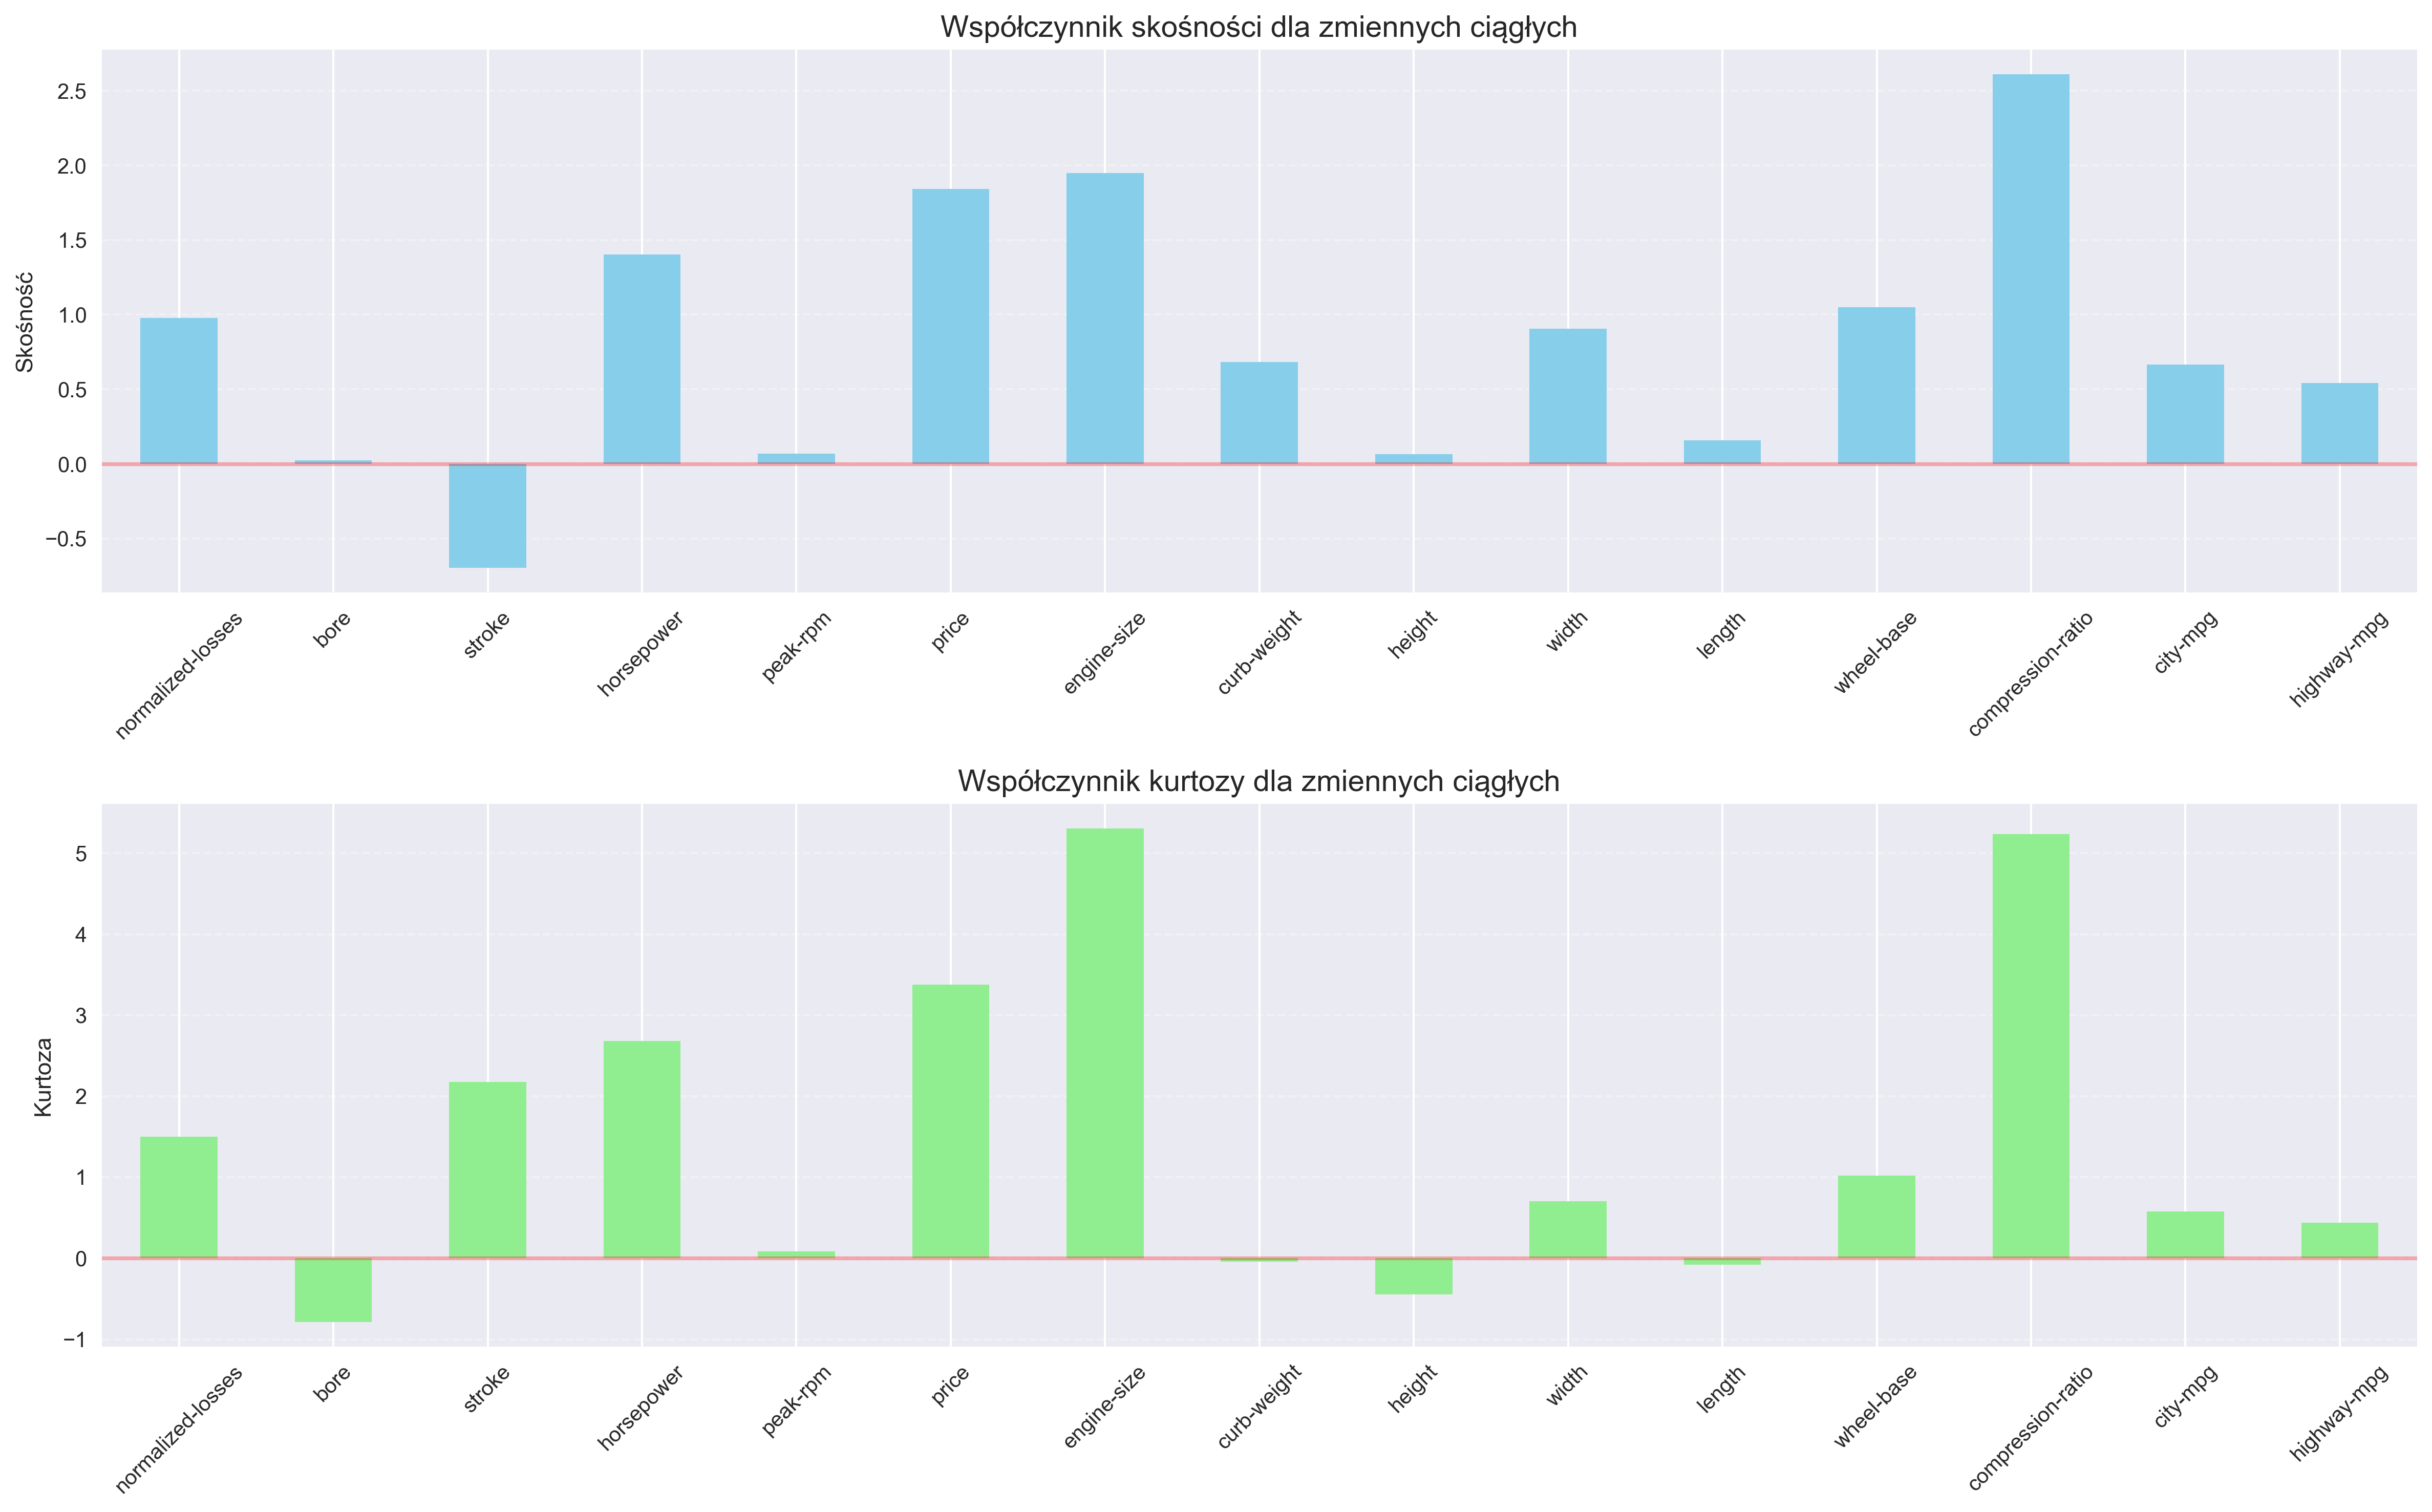
\includegraphics[width=0.9\textwidth]{figures/skosnosc_kurtoza.png}
    \caption{Współczynniki skosnosci i kurtozy dla analizowanych zmiennych}
    \label{fig:skosnosc_kurtoza}
\end{figure}

Na podstawie wykresu skosnosci (Rys.~\ref{fig:skosnosc_kurtoza}) można zauważyc, że większosc zmiennych charakteryzuje się prawostronną asymetrią, co wskazuje na obecnosc wartosci odstających po prawej stronie rozkładu. Szczególnie wysokie wartosci skosnosci można zaobserwowac dla zmiennych `price` i `normalized-losses`.

\begin{figure}[H]
    \centering
    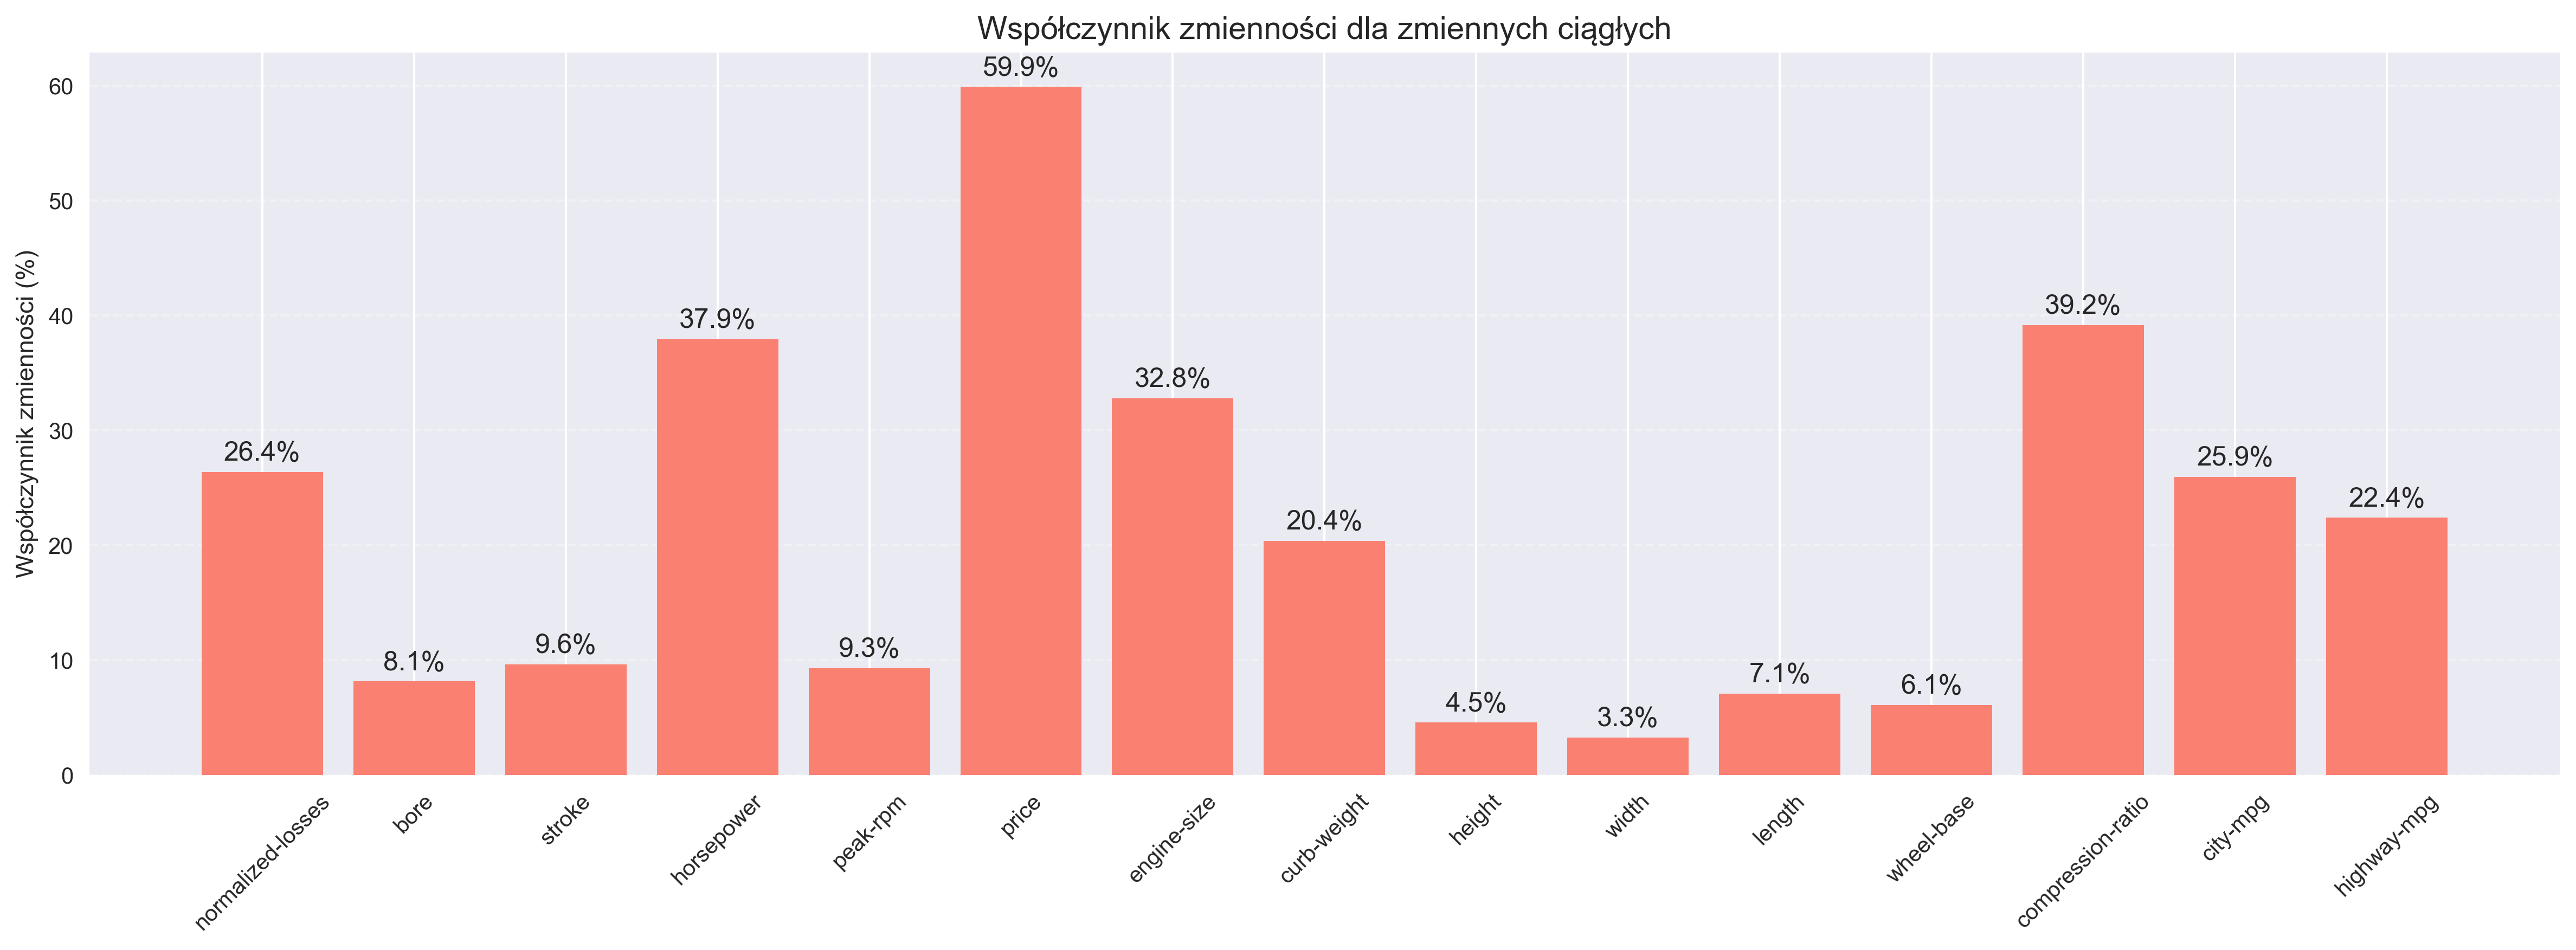
\includegraphics[width=0.9\textwidth]{figures/wspolczynnik_zmiennosci.png}
    \caption{Współczynniki zmiennosci dla analizowanych zmiennych}
    \label{fig:wspolczynnik_zmiennosci}
\end{figure}

Współczynnik zmiennosci (Rys.~\ref{fig:wspolczynnik_zmiennosci}) pozwala ocenic stopień zróżnicowania danych względem sredniej. Najwyższą zmiennoscią charakteryzują się zmienne `normalized-losses` i `price`, co wskazuje na dużą różnorodnosc w tych atrybutach.

\begin{figure}[H]
    \centering
    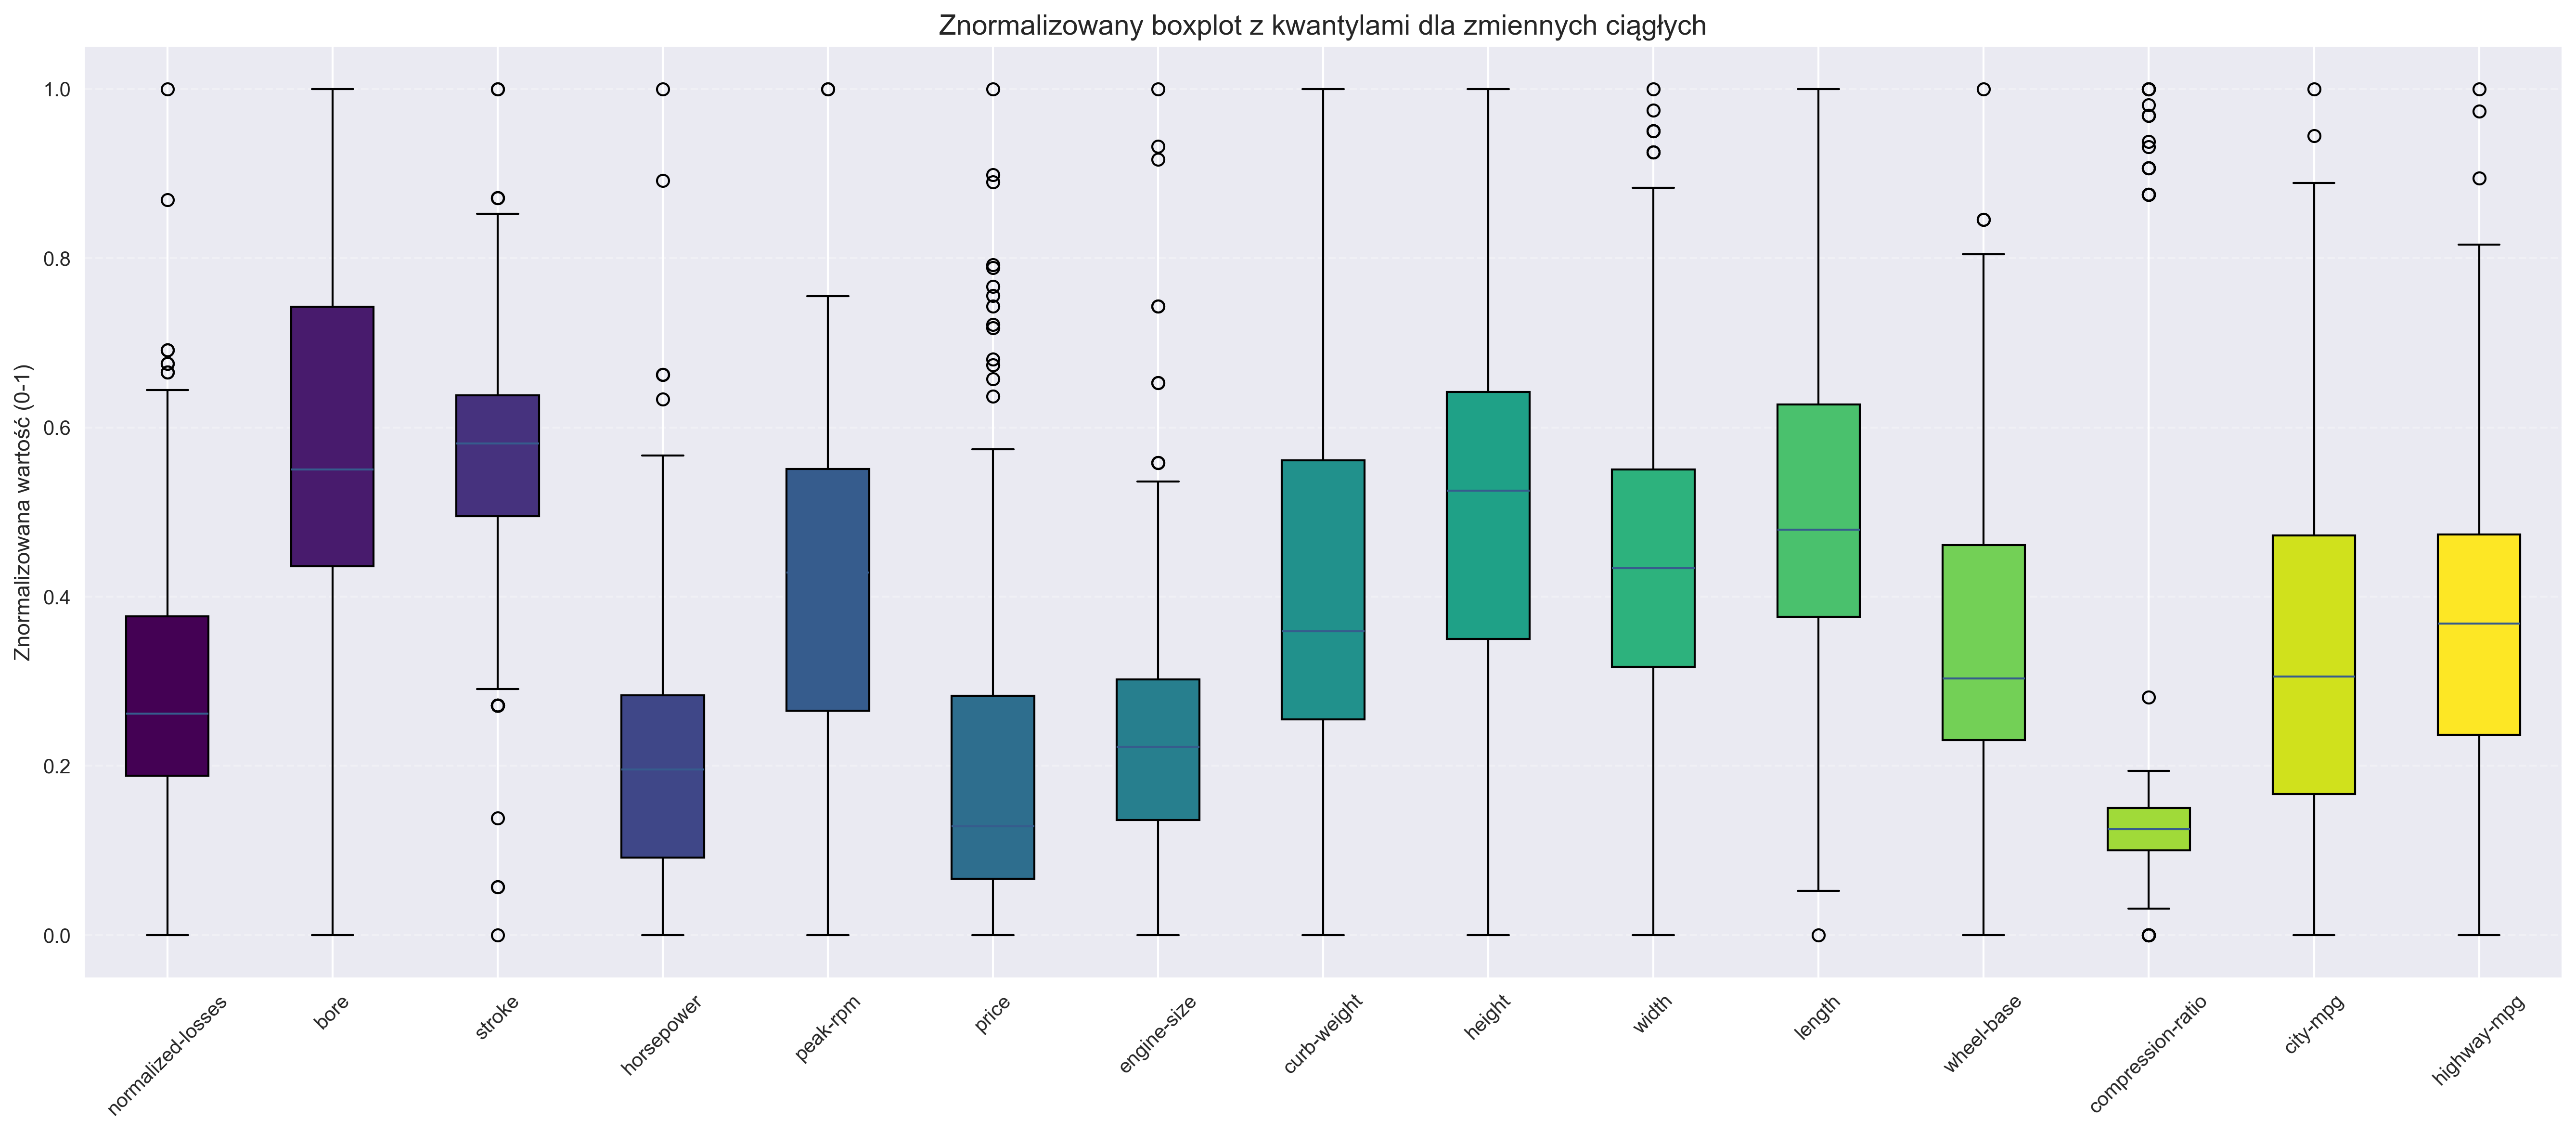
\includegraphics[width=0.9\textwidth]{figures/boxplots_znormalizowane.png}
    \caption{Znormalizowane boxploty dla zmiennych ciągłych}
    \label{fig:boxplots_znormalizowane}
\end{figure}

Znormalizowane boxploty (Rys.~\ref{fig:boxplots_znormalizowane}) umożliwiają porównanie rozkładów zmiennych o różnych skalach. Widoczne są wartosci odstające w wielu zmiennych, szczególnie w `compression-ratio` i `peak-rpm`.

\begin{figure}[H]
    \centering
    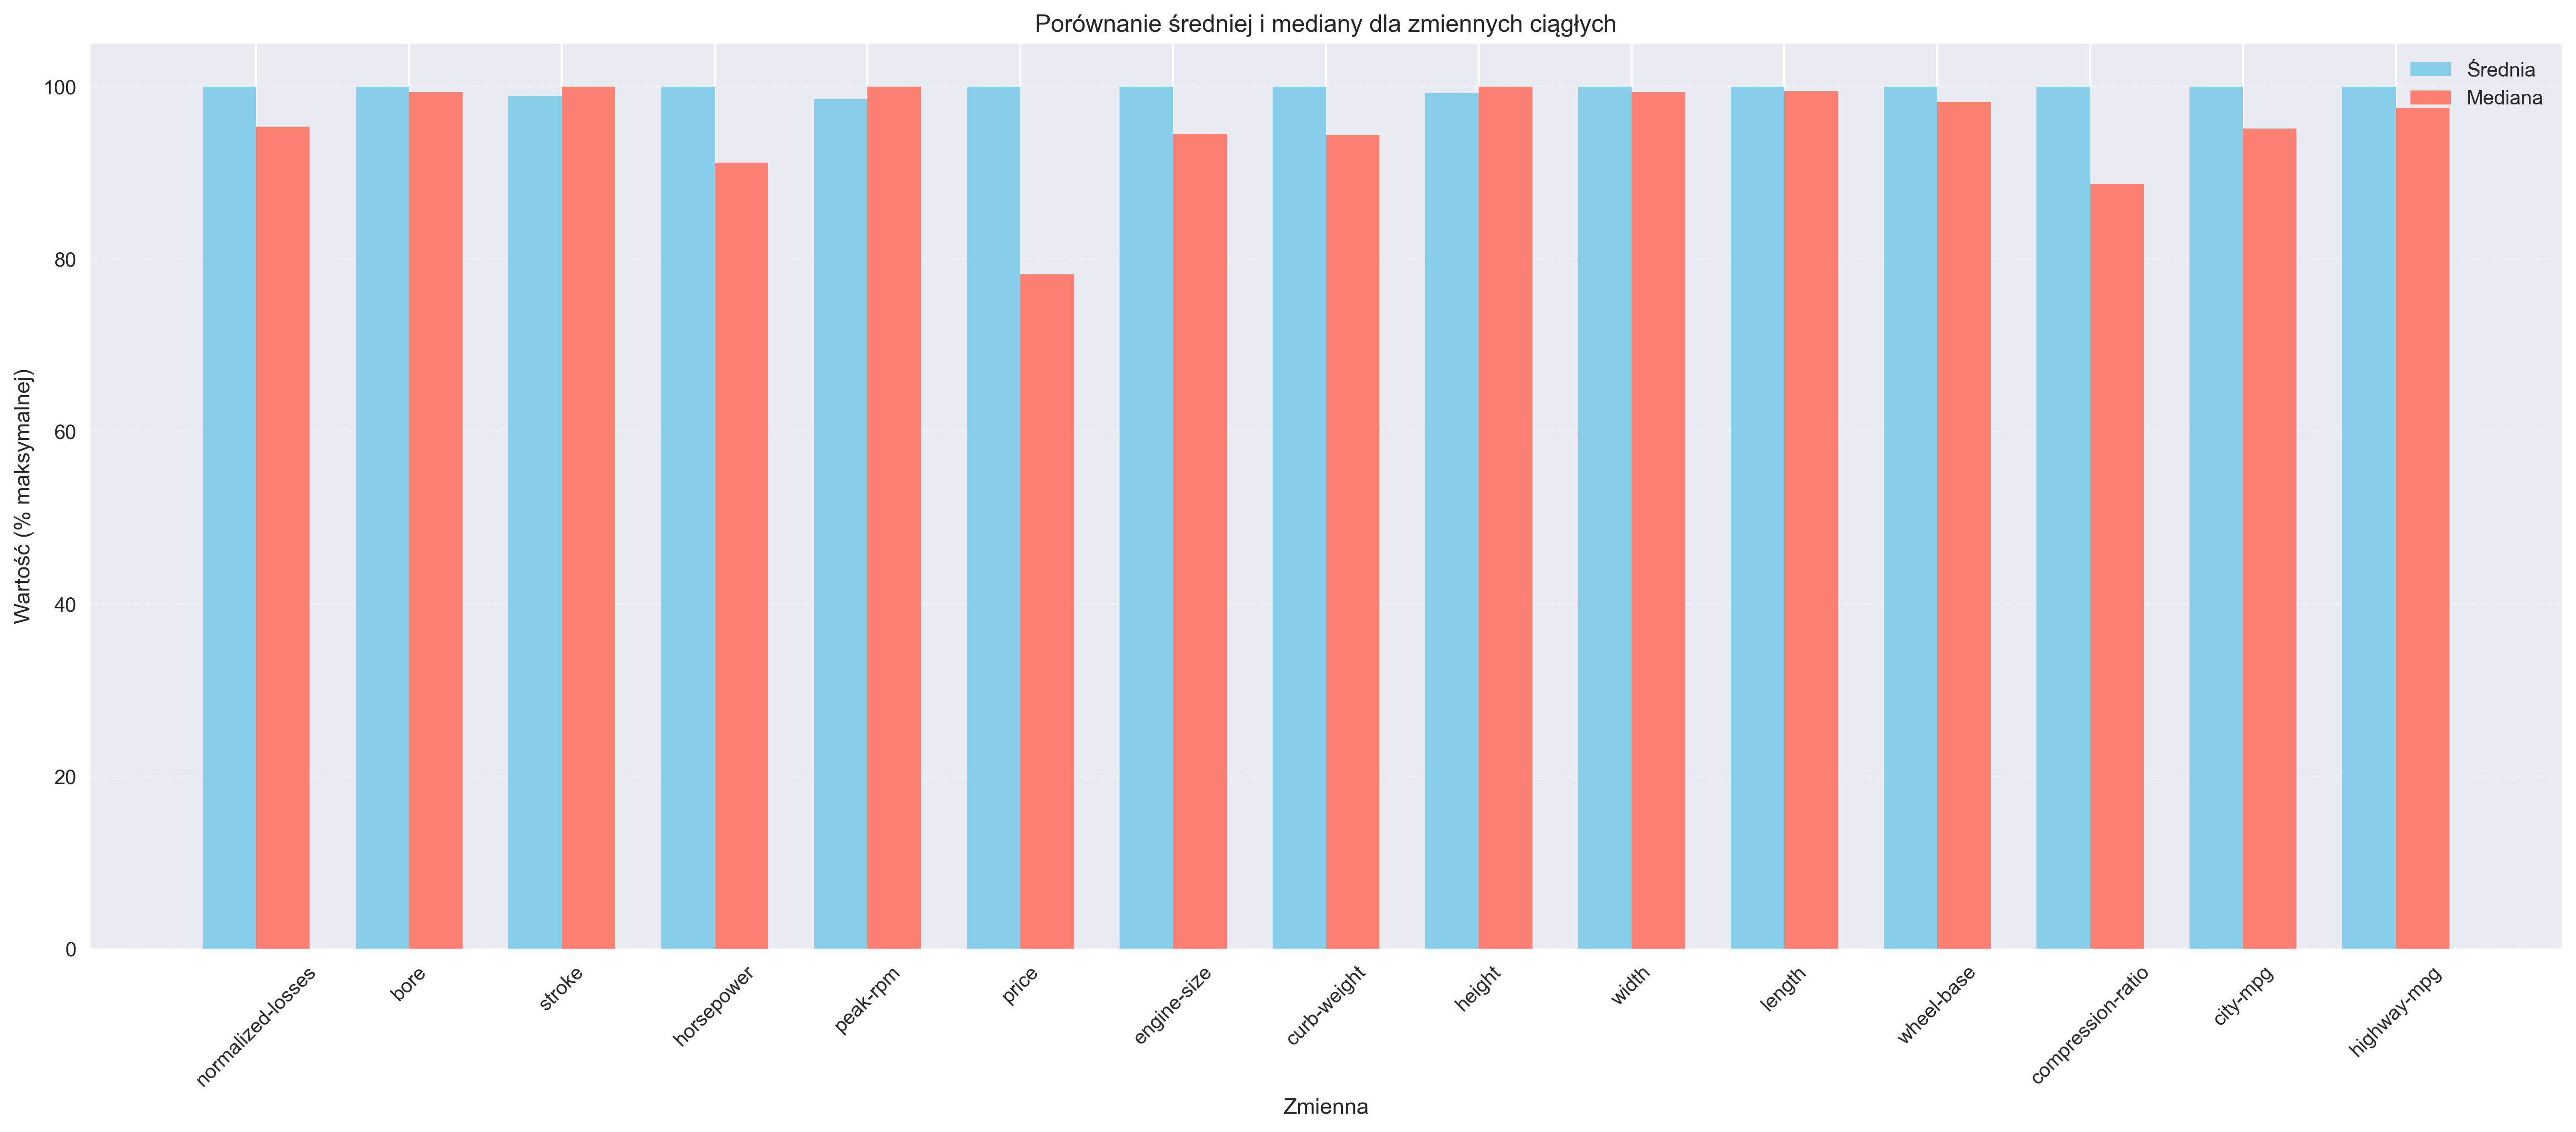
\includegraphics[width=0.9\textwidth]{figures/srednia_vs_mediana.png}
    \caption{Porównanie sredniej i mediany dla zmiennych ciągłych}
    \label{fig:srednia_vs_mediana}
\end{figure}

Porównanie sredniej i mediany (Rys.~\ref{fig:srednia_vs_mediana}) potwierdza asymetrię rozkładów. W przypadku większosci zmiennych srednia przewyższa medianę, co jest charakterystyczne dla rozkładów z prawostronną asymetrią.

\subsection{Kod implementujący estymację punktową}
\begin{lstlisting}[language=Python, caption=Funkcja do obliczania parametrów rozkładu]
def calculate_distribution_parameters(data):
    params = {}
    # Miary tendencji centralnej
    params['srednia'] = data.mean()
    params['srednia geometryczna'] = stats.gmean(data) if all(data > 0) else np.nan
    params['srednia harmoniczna'] = stats.hmean(data) if all(data > 0) else np.nan
    params['Mediana'] = data.median()
    params['Moda'] = data.mode()[0]

    # Miary rozproszenia
    params['Wariancja (próbkowa)'] = data.var(ddof=1)
    params['Wariancja (populacyjna)'] = data.var(ddof=0)
    params['Odchylenie standardowe (próbkowe)'] = data.std(ddof=1)
    params['Odchylenie standardowe (populacyjne)'] = data.std(ddof=0)
    params['Odchylenie przeciętne'] = (data - data.mean()).abs().mean()
    params['Odchylenie cwiartkowe'] = (np.percentile(data, 75) - np.percentile(data, 25))/2
    params['Współczynnik zmiennosci'] = (data.std()/data.mean())*100 if data.mean() != 0 else np.nan

    # Miary kształtu rozkładu
    params['Skosnosc'] = stats.skew(data, bias=False)
    params['Współczynnik asymetrii Pearsona'] = 3 * (data.mean() - data.median()) / data.std() if data.std() != 0 else np.nan
    params['Kurtoza'] = stats.kurtosis(data, bias=False)
    params['Eksces'] = stats.kurtosis(data, bias=False, fisher=True)  

    # Kwantyle i miary pozycyjne
    params['Minimum'] = data.min()
    params['Maximum'] = data.max()
    params['Zakres'] = data.max() - data.min()
    params['Q1 (25%)'] = np.percentile(data, 25)
    params['Q2 (50%)'] = np.percentile(data, 50)
    params['Q3 (75%)'] = np.percentile(data, 75)
    params['P10 (10%)'] = np.percentile(data, 10)
    params['P90 (90%)'] = np.percentile(data, 90)
    params['P95 (95%)'] = np.percentile(data, 95)
    params['P99 (99%)'] = np.percentile(data, 99)
    params['IQR'] = np.percentile(data, 75) - np.percentile(data, 25)

    # Dodatkowe statystyki
    params['Błąd standardowy sredniej'] = data.std(ddof=1) / np.sqrt(len(data))
    params['Suma'] = data.sum()
    params['Liczba obserwacji'] = len(data)
    params['Liczba unikalnych wartosci'] = data.nunique()

    # Momenty centralne
    params['Moment centralny rzędu 1'] = np.mean((data - data.mean()) ** 1)
    params['Moment centralny rzędu 2'] = np.mean((data - data.mean()) ** 2)
    params['Moment centralny rzędu 3'] = np.mean((data - data.mean()) ** 3)
    params['Moment centralny rzędu 4'] = np.mean((data - data.mean()) ** 4)

    return params
\end{lstlisting}

\section{Estymacja parametrów (przedziałowa)}

W tej sekcji zostały obliczone przedziały ufnosci dla sredniej i wariancji z wykorzystaniem różnych metod:
\begin{itemize}
    \item Przedziały ufnosci dla sredniej obliczone metodą parametryczną (opartą o rozkład t-Studenta)
    \item Przedziały ufnosci dla sredniej obliczone metodami nieparametrycznymi (bootstrap percentylowy oraz bootstrap BCa)
    \item Przedziały ufnosci dla wariancji obliczone metodą parametryczną (opartą o rozkład chi-kwadrat)
\end{itemize}

\begin{figure}[H]
    \centering
    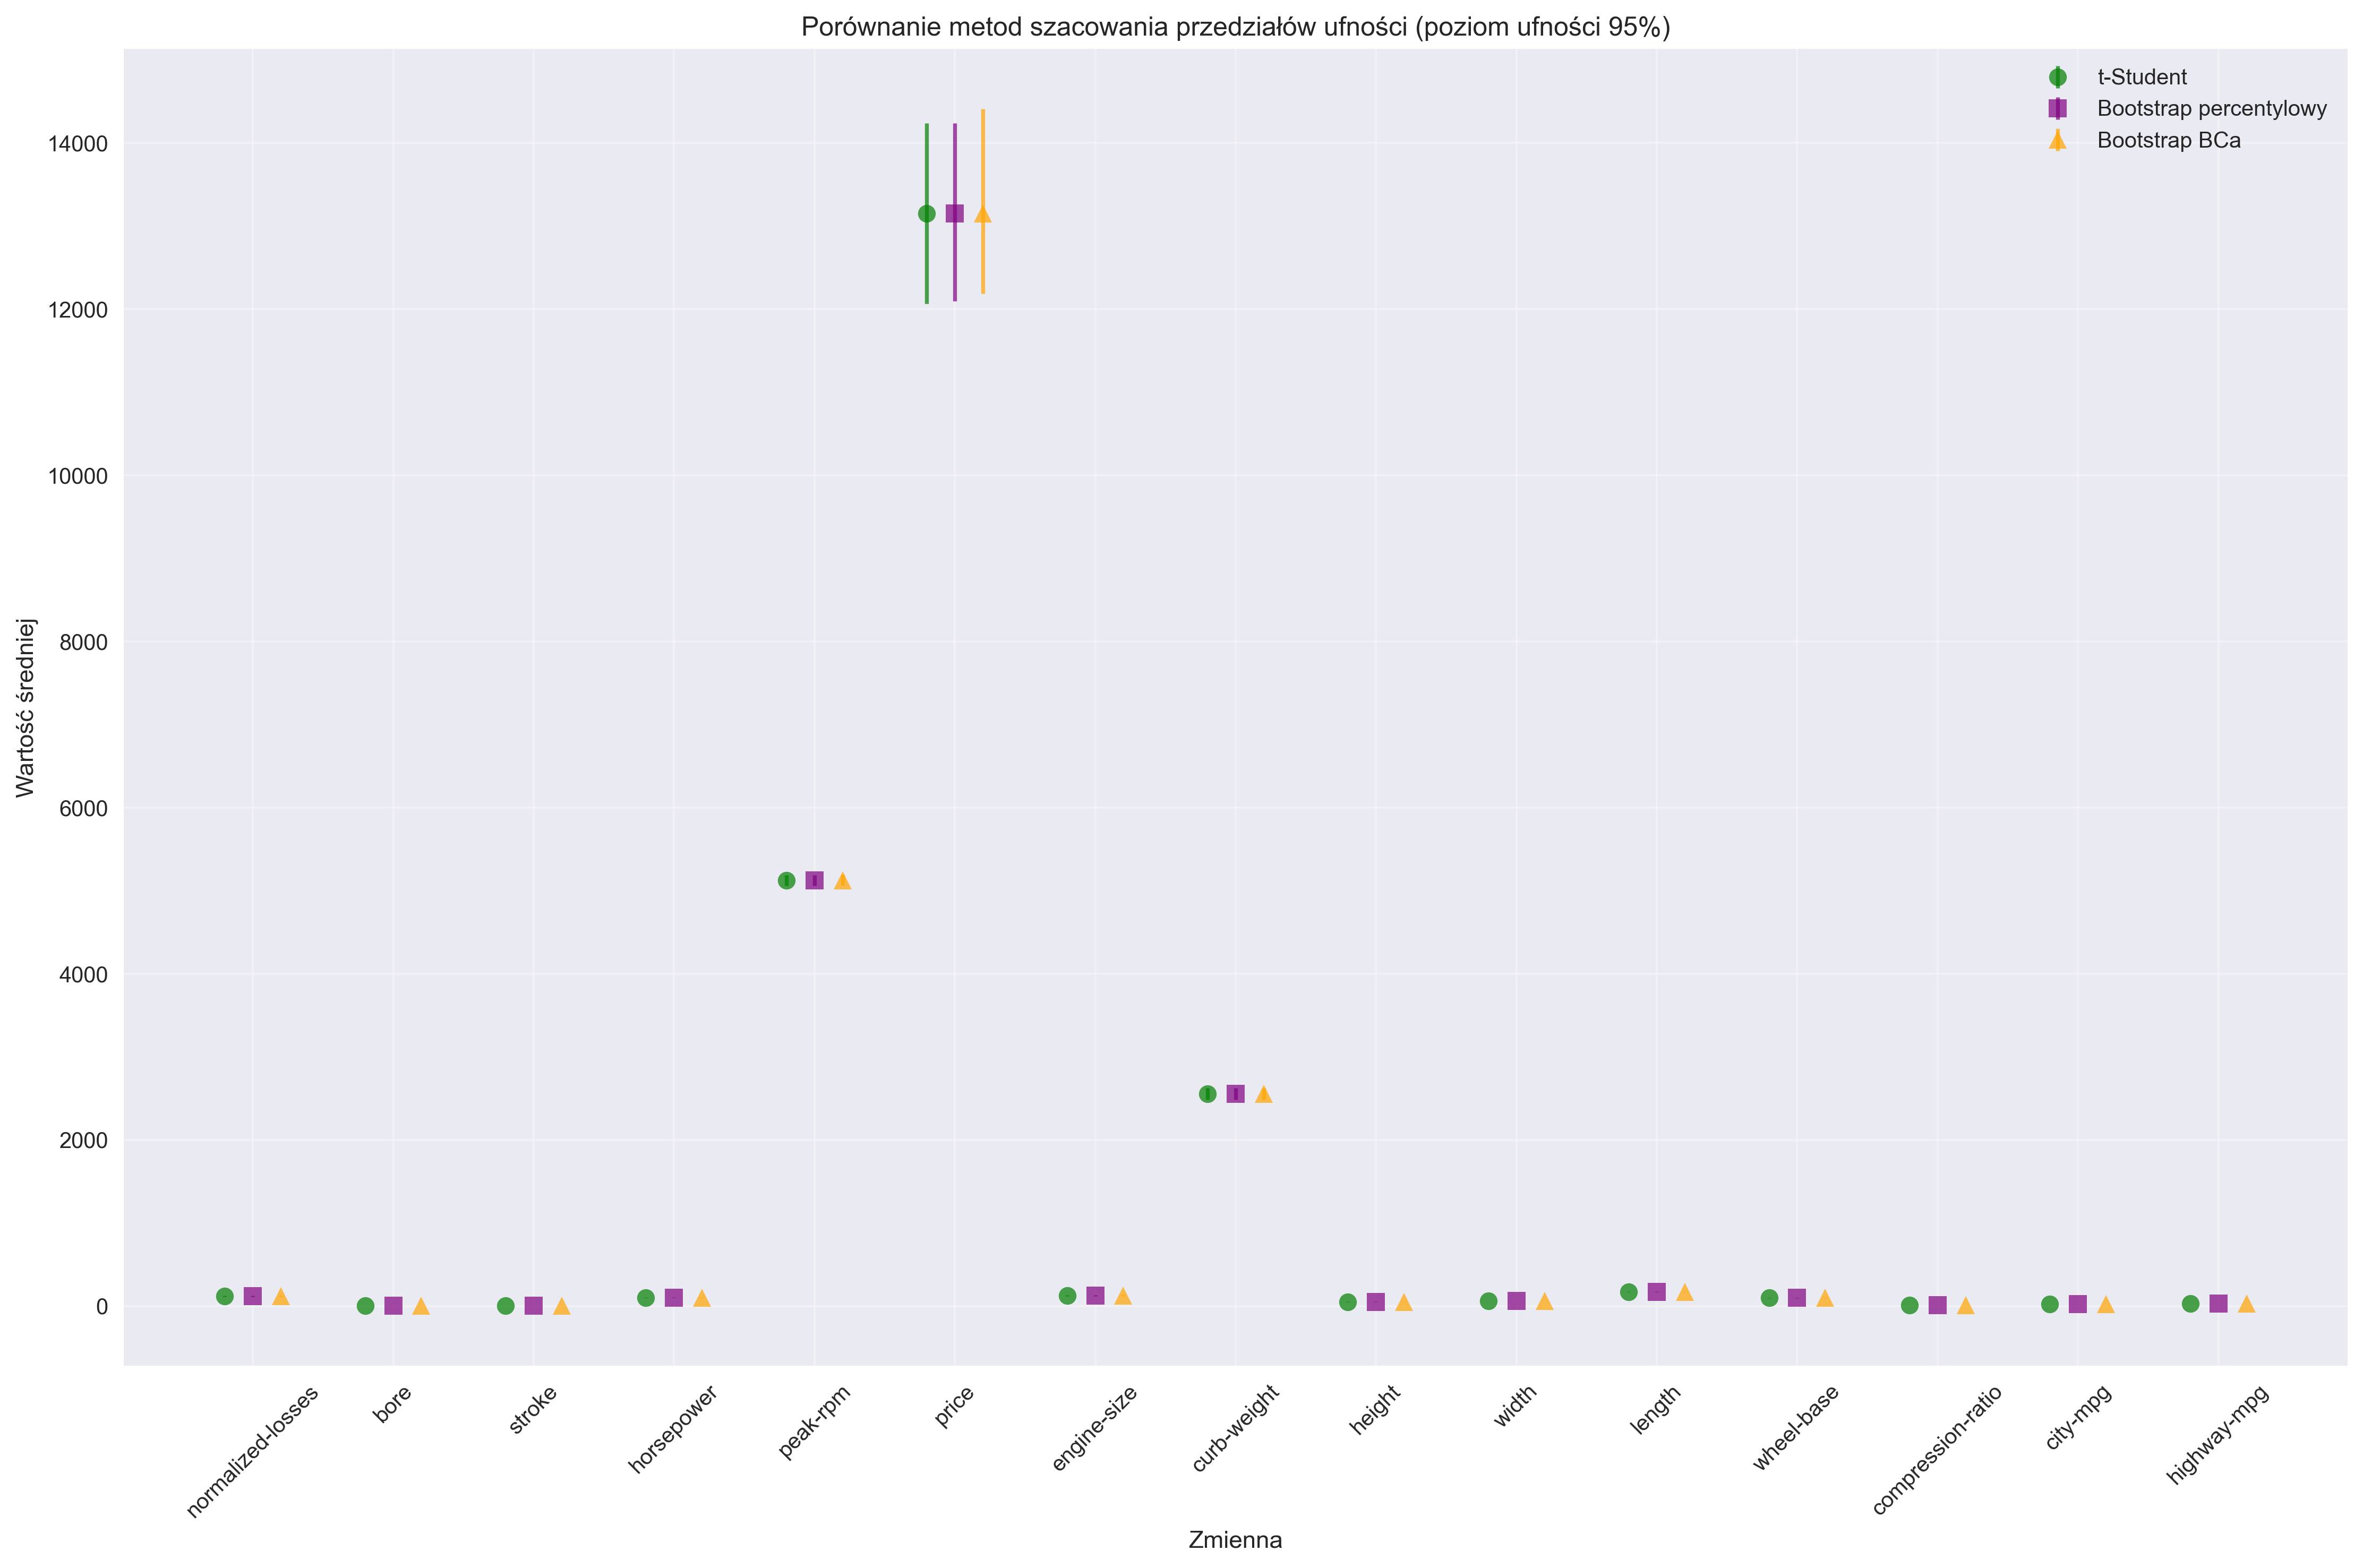
\includegraphics[width=0.9\textwidth]{figures/ci_methods_comparison.png}
    \caption{Porównanie metod szacowania przedziałów ufnosci dla sredniej}
    \label{fig:ci_methods_comparison}
\end{figure}

Rysunek~\ref{fig:ci_methods_comparison} prezentuje porównanie trzech metod wyznaczania przedziałów ufnosci dla sredniej. Można zauważyc, że metoda bootstrapowa BCa często generuje niesymetryczne przedziały ufnosci, co jest korzystne w przypadku rozkładów o wyraźnej asymetrii.

\begin{figure}[H]
    \centering
    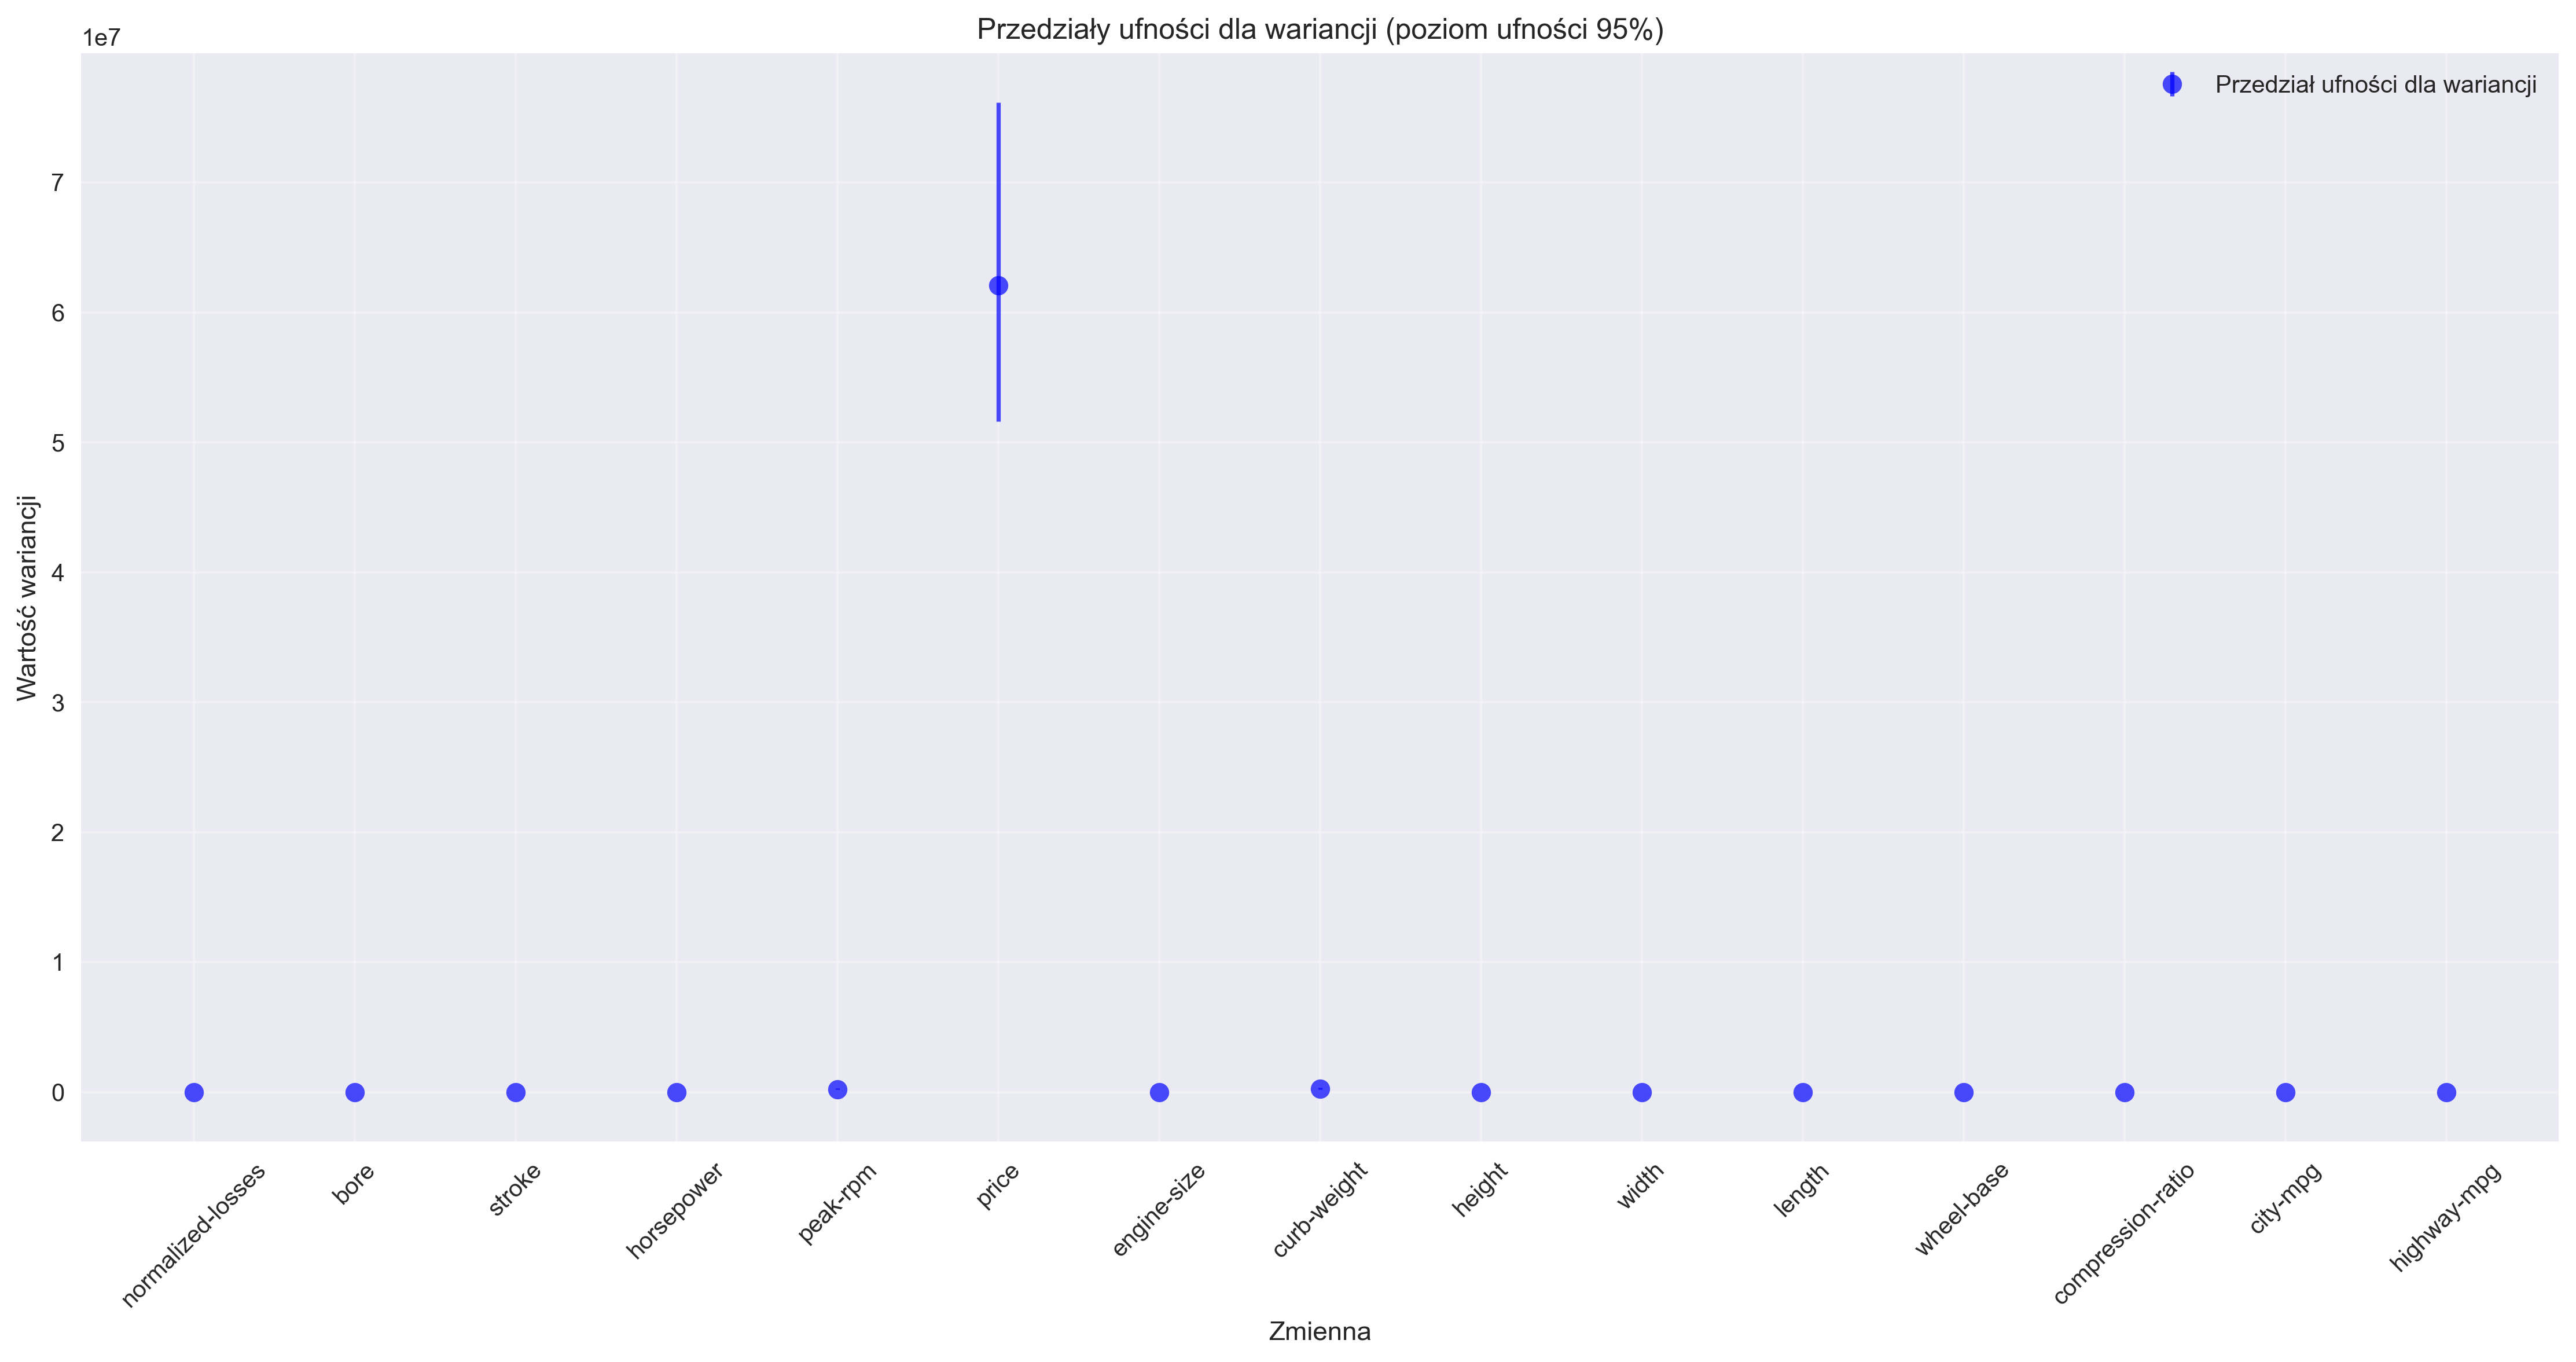
\includegraphics[width=0.9\textwidth]{figures/variance_ci.png}
    \caption{Przedziały ufnosci dla wariancji}
    \label{fig:variance_ci}
\end{figure}

Rysunek~\ref{fig:variance_ci} przedstawia przedziały ufnosci dla wariancji. Zmienne o wysokiej wariancji, takie jak `price`, mają szersze przedziały ufnosci, co wskazuje na większą niepewnosc estymacji.

\begin{figure}[H]
    \centering
    \begin{subfigure}[b]{0.48\textwidth}
        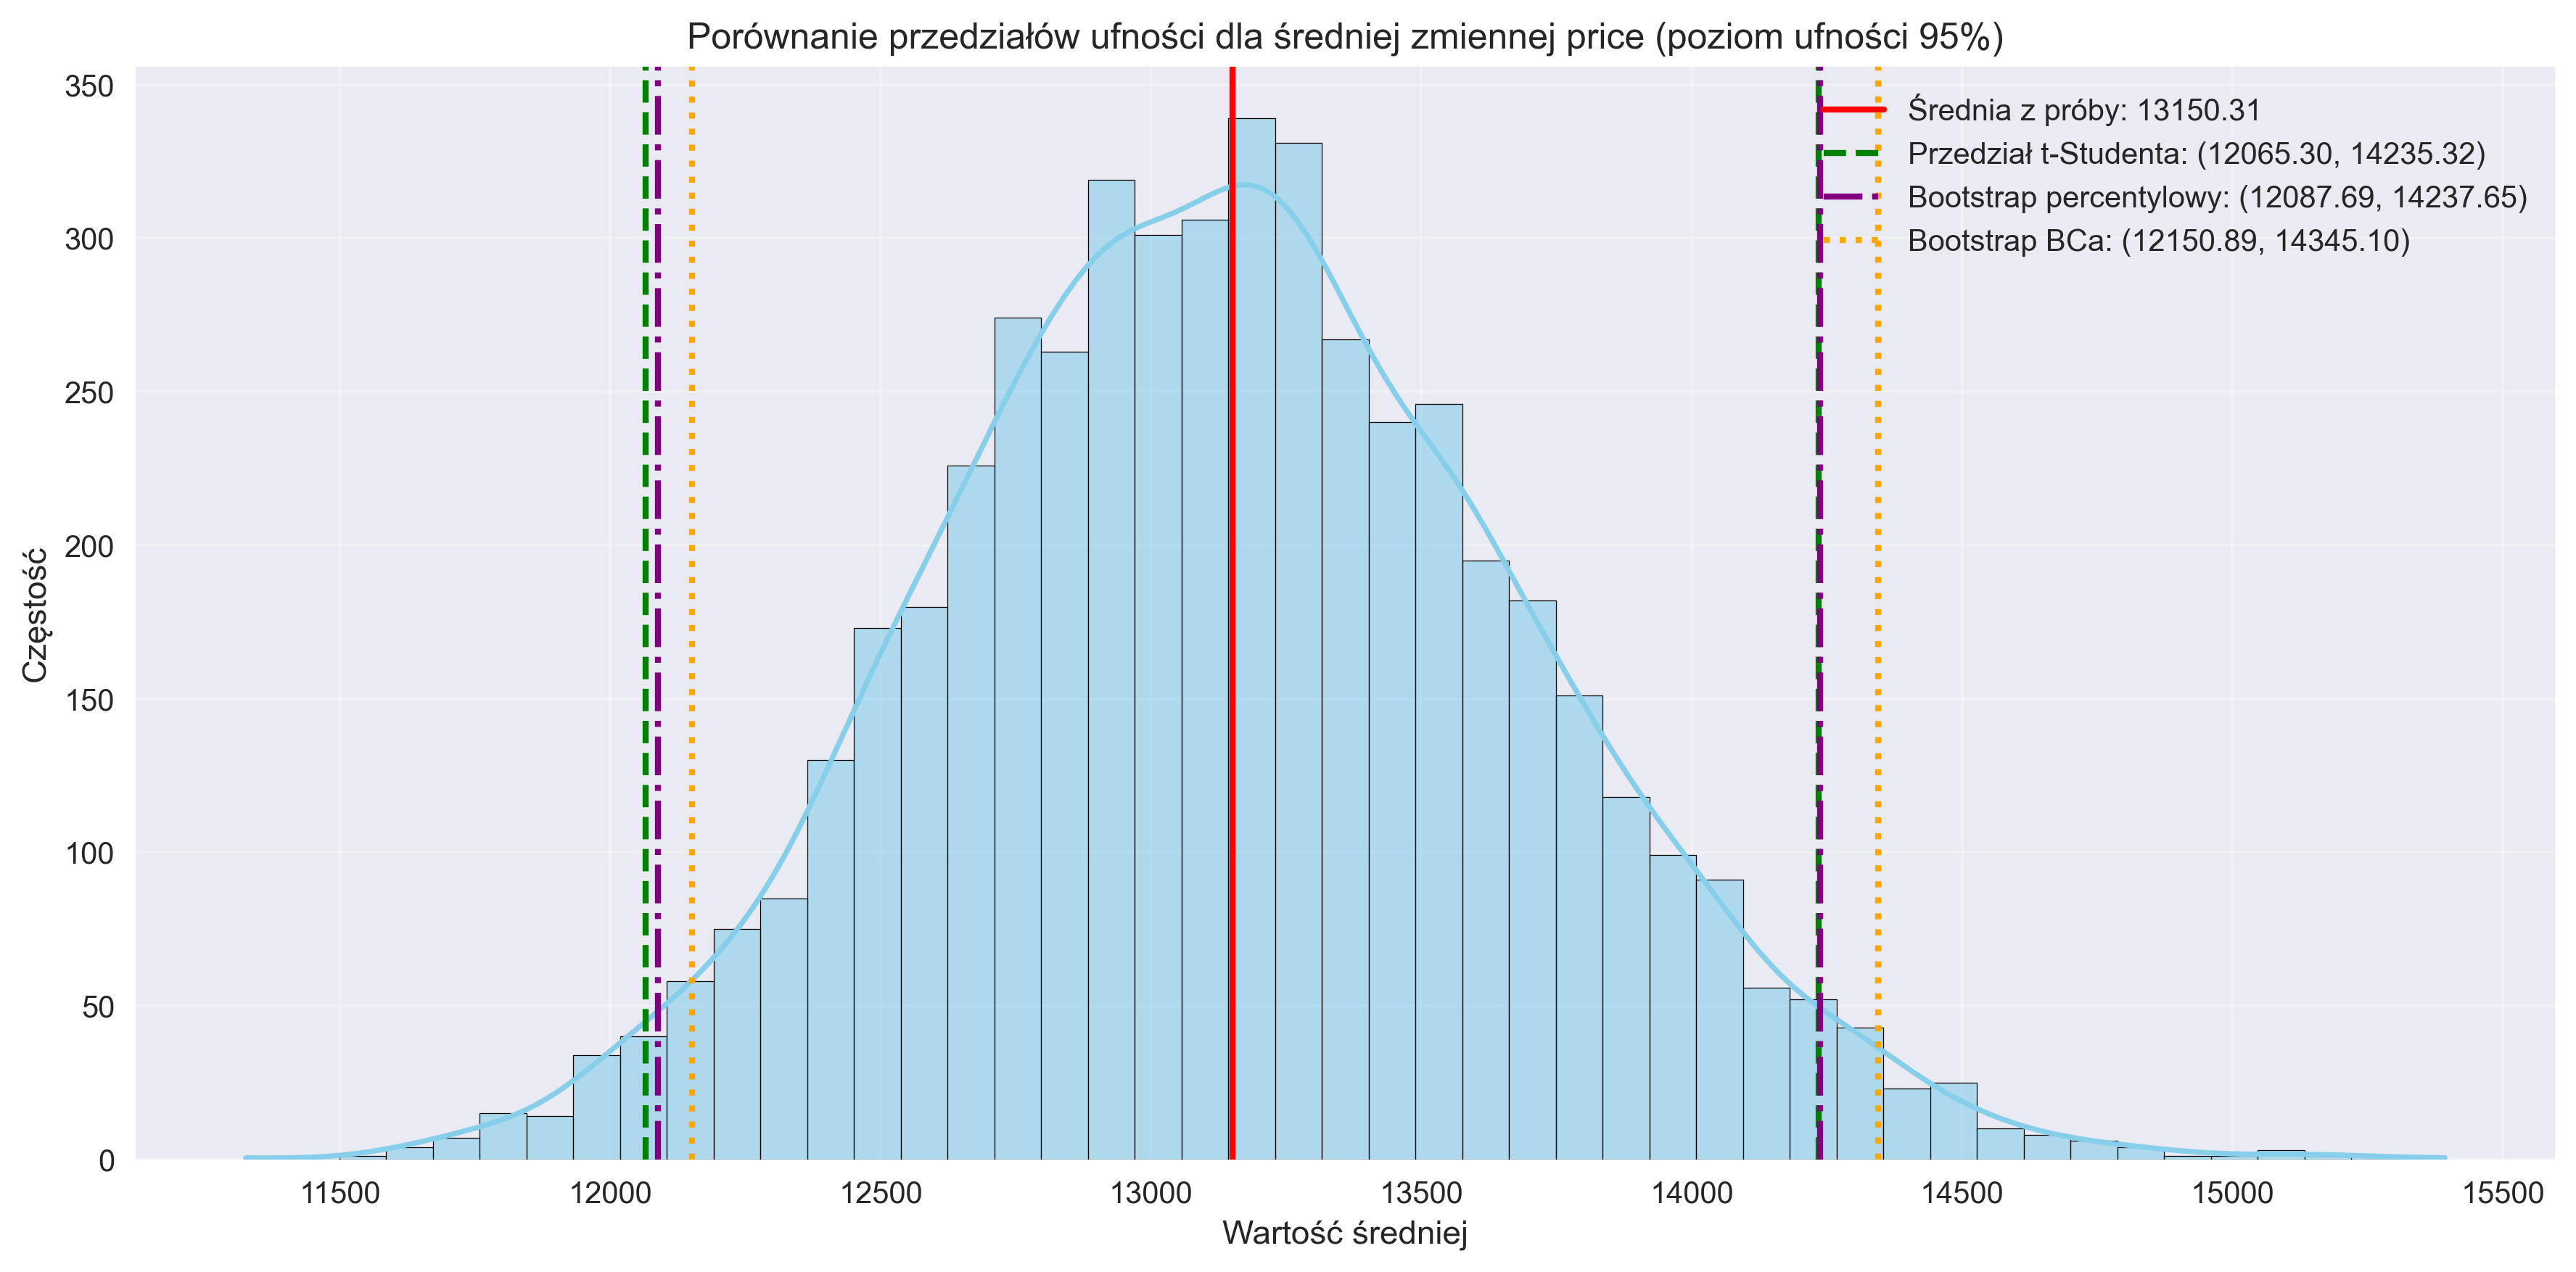
\includegraphics[width=\textwidth]{figures/ci_comparison_price.png}
        \caption{Przedziały ufnosci dla zmiennej price}
    \end{subfigure}
    \hfill
    \begin{subfigure}[b]{0.48\textwidth}
        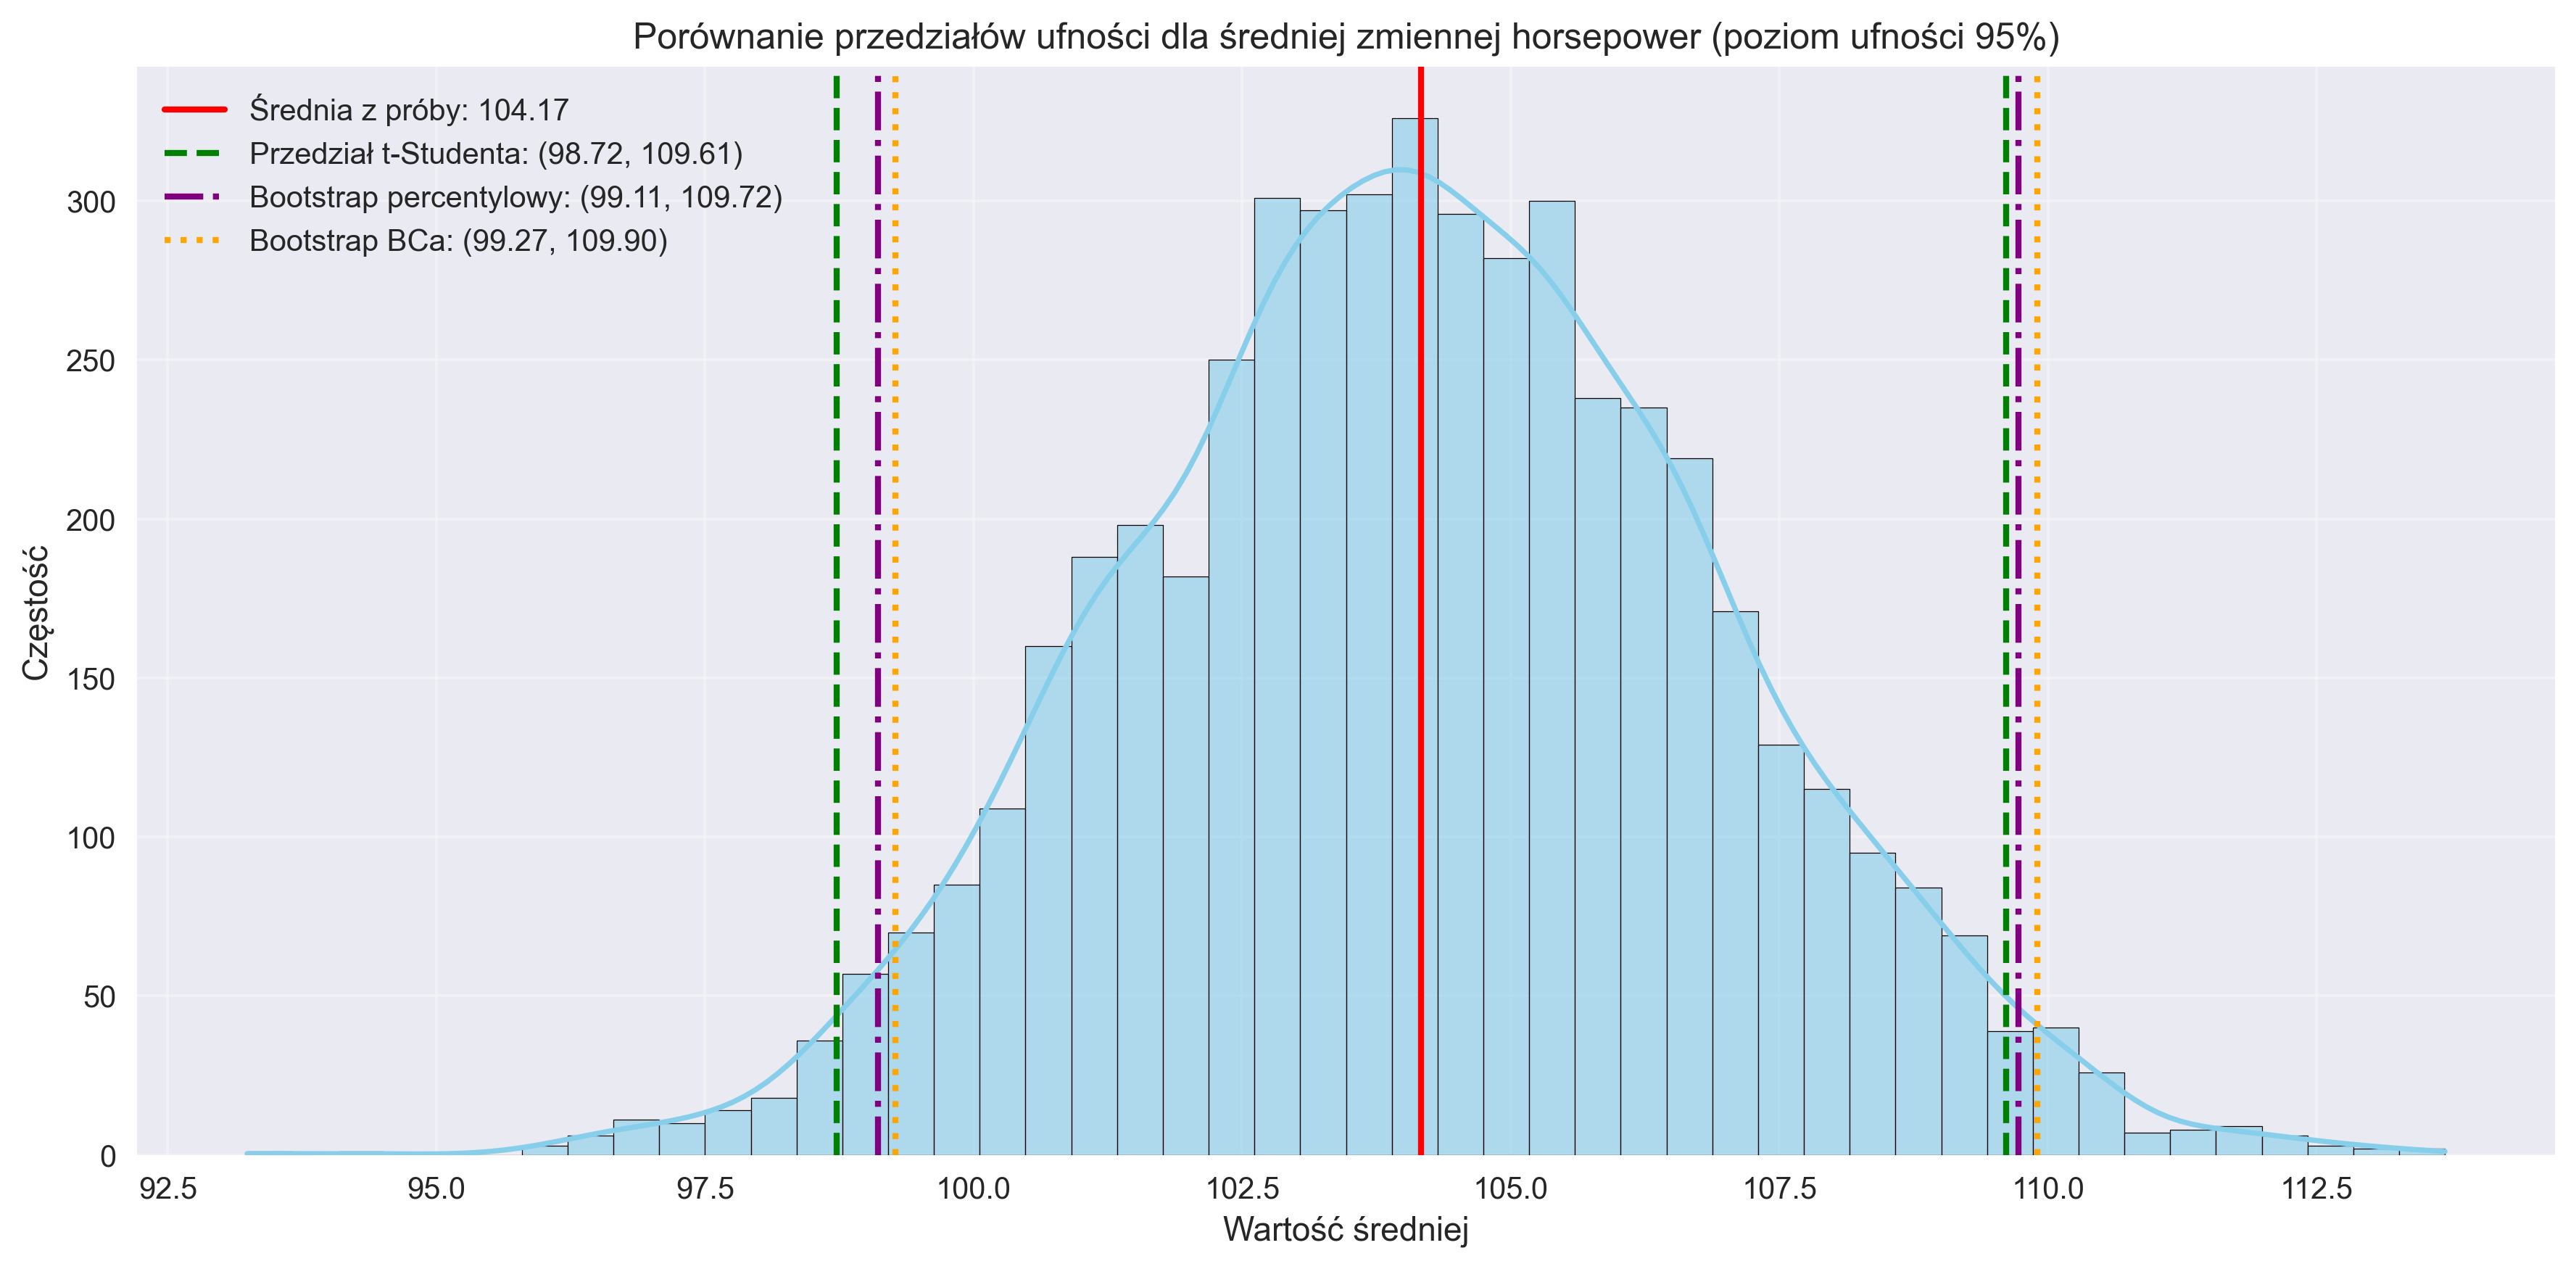
\includegraphics[width=\textwidth]{figures/ci_comparison_horsepower.png}
        \caption{Przedziały ufnosci dla zmiennej horsepower}
    \end{subfigure}
    \caption{Porównanie metod wyznaczania przedziałów ufnosci dla wybranych zmiennych}
    \label{fig:ci_comparison_selected}
\end{figure}

Szczegółowa analiza dla zmiennych `price` i `horsepower` (Rys.~\ref{fig:ci_comparison_selected}) pokazuje rozkład bootstrapowy sredniej oraz różne metody estymacji przedziałów ufnosci. Widoczne są różnice w szerokosci i położeniu przedziałów w zależnosci od zastosowanej metody.

\subsection{Kod implementujący estymację przedziałową}
\begin{lstlisting}[language=Python, caption=Funkcje do obliczania przedziałów ufnosci]
# Funkcje do obliczania przedziałów ufnosci parametrycznymi metodami
def mean_confidence_interval_t(data, confidence=0.95):
    n = len(data)
    mean = np.mean(data)
    std_err = np.std(data, ddof=1) / np.sqrt(n)
    t_critical = stats.t.ppf((1 + confidence) / 2, n-1)
    margin_of_error = t_critical * std_err
    return (mean - margin_of_error, mean + margin_of_error)

def variance_confidence_interval(data, confidence=0.95):
    n = len(data)
    var = np.var(data, ddof=1)
    chi2_lower = stats.chi2.ppf((1 - confidence) / 2, n-1)
    chi2_upper = stats.chi2.ppf((1 + confidence) / 2, n-1)
    var_lower = (n-1) * var / chi2_upper
    var_upper = (n-1) * var / chi2_lower
    return (var_lower, var_upper)

# Funkcje do obliczania przedziałów ufnosci metodą bootstrap
def bootstrap_confidence_interval(data, n_bootstrap=5000, confidence=0.95):
    bootstrap_means = []
    for _ in range(n_bootstrap):
        bootstrap_sample = resample(data, replace=True, n_samples=len(data))
        bootstrap_means.append(np.mean(bootstrap_sample))
    lower_percentile = (1 - confidence) / 2 * 100
    upper_percentile = (1 + confidence) / 2 * 100
    return np.percentile(bootstrap_means, [lower_percentile, upper_percentile])

def bootstrap_bca_interval(data, statistic=np.mean, n_bootstrap=5000, confidence=0.95):
    theta_hat = statistic(data)
    bootstrap_replicates = []
    for _ in range(n_bootstrap):
        bootstrap_sample = resample(data, replace=True, n_samples=len(data))
        bootstrap_replicates.append(statistic(bootstrap_sample))
    
    prop_less_than_theta_hat = np.mean([1 if t < theta_hat else 0 for t in bootstrap_replicates])
    z0 = stats.norm.ppf(prop_less_than_theta_hat)
    
    jackknife_replicates = []
    for i in range(len(data)):
        jack_sample = np.delete(data, i)
        jackknife_replicates.append(statistic(jack_sample))
    
    jack_mean = np.mean(jackknife_replicates)
    num = np.sum([(jack_mean - jt)**3 for jt in jackknife_replicates])
    den = 6.0 * np.sum([(jack_mean - jt)**2 for jt in jackknife_replicates])**1.5
    
    if abs(den) < 1e-10:
        a = 0
    else:
        a = num / den
    
    alpha = (1 - confidence) / 2
    z_alpha = stats.norm.ppf(alpha)
    z_1_minus_alpha = stats.norm.ppf(1 - alpha)
    
    p_lower = stats.norm.cdf(z0 + (z0 + z_alpha) / (1 - a * (z0 + z_alpha)))
    p_upper = stats.norm.cdf(z0 + (z0 + z_1_minus_alpha) / (1 - a * (z0 + z_1_minus_alpha)))
    
    lower_percentile = 100 * p_lower
    upper_percentile = 100 * p_upper
    
    return np.percentile(bootstrap_replicates, [lower_percentile, upper_percentile])
\end{lstlisting}

\section{Różne wykresy dla analizy zmiennych}

Wizualizacja danych jest kluczowym elementem analizy statystycznej, umożliwiającym lepsze zrozumienie charakterystyk badanych zmiennych. W tej sekcji przedstawiono różnorodne typy wykresów, które pomagają w odkrywaniu wzorców i zależnosci w danych.

\begin{figure}[H]
    \centering
    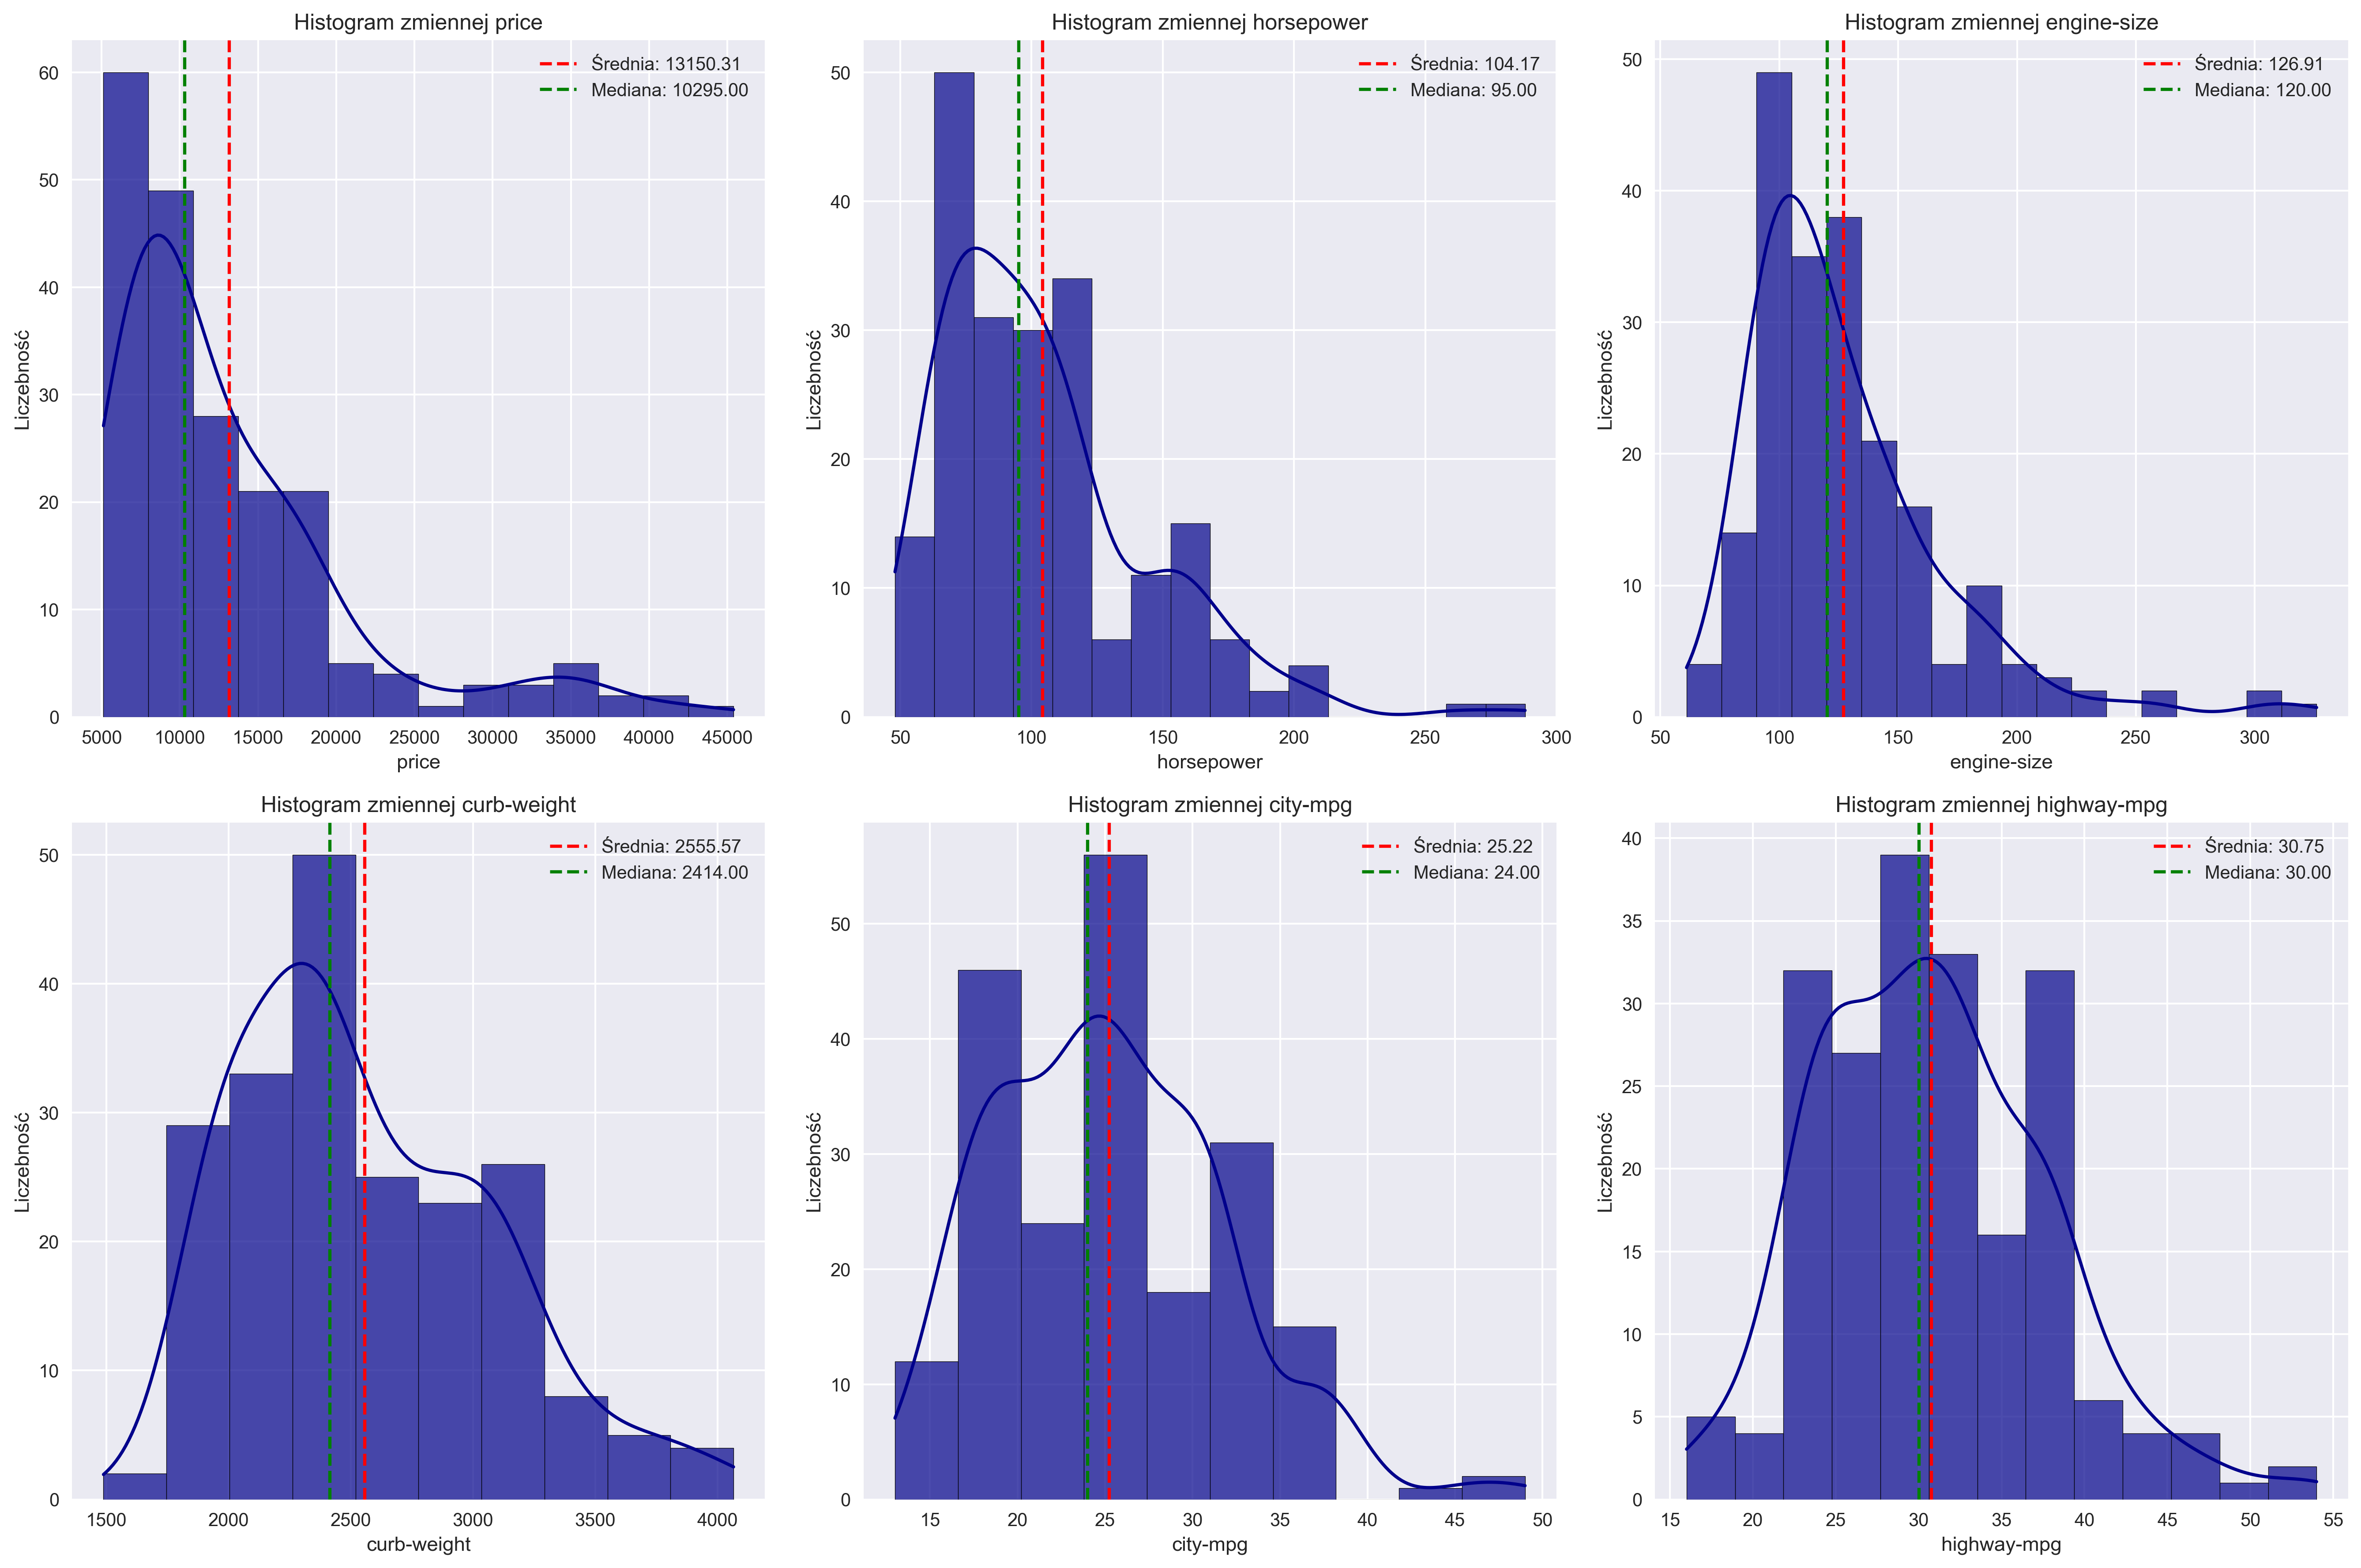
\includegraphics[width=0.9\textwidth]{figures/histograms.png}
    \caption{Histogramy dla wybranych zmiennych}
    \label{fig:histograms}
\end{figure}

Histogramy (Rys.~\ref{fig:histograms}) pokazują rozkład częstosci występowania wartosci dla wybranych zmiennych. Na wykresach oznaczono srednią (czerwona linia przerywana) oraz medianę (zielona linia przerywana). Widoczne są różnice w kształcie rozkładów, z wyraźną prawostronną asymetrią dla zmiennych `price`, `horsepower` i `engine-size`.

\begin{figure}[H]
    \centering
    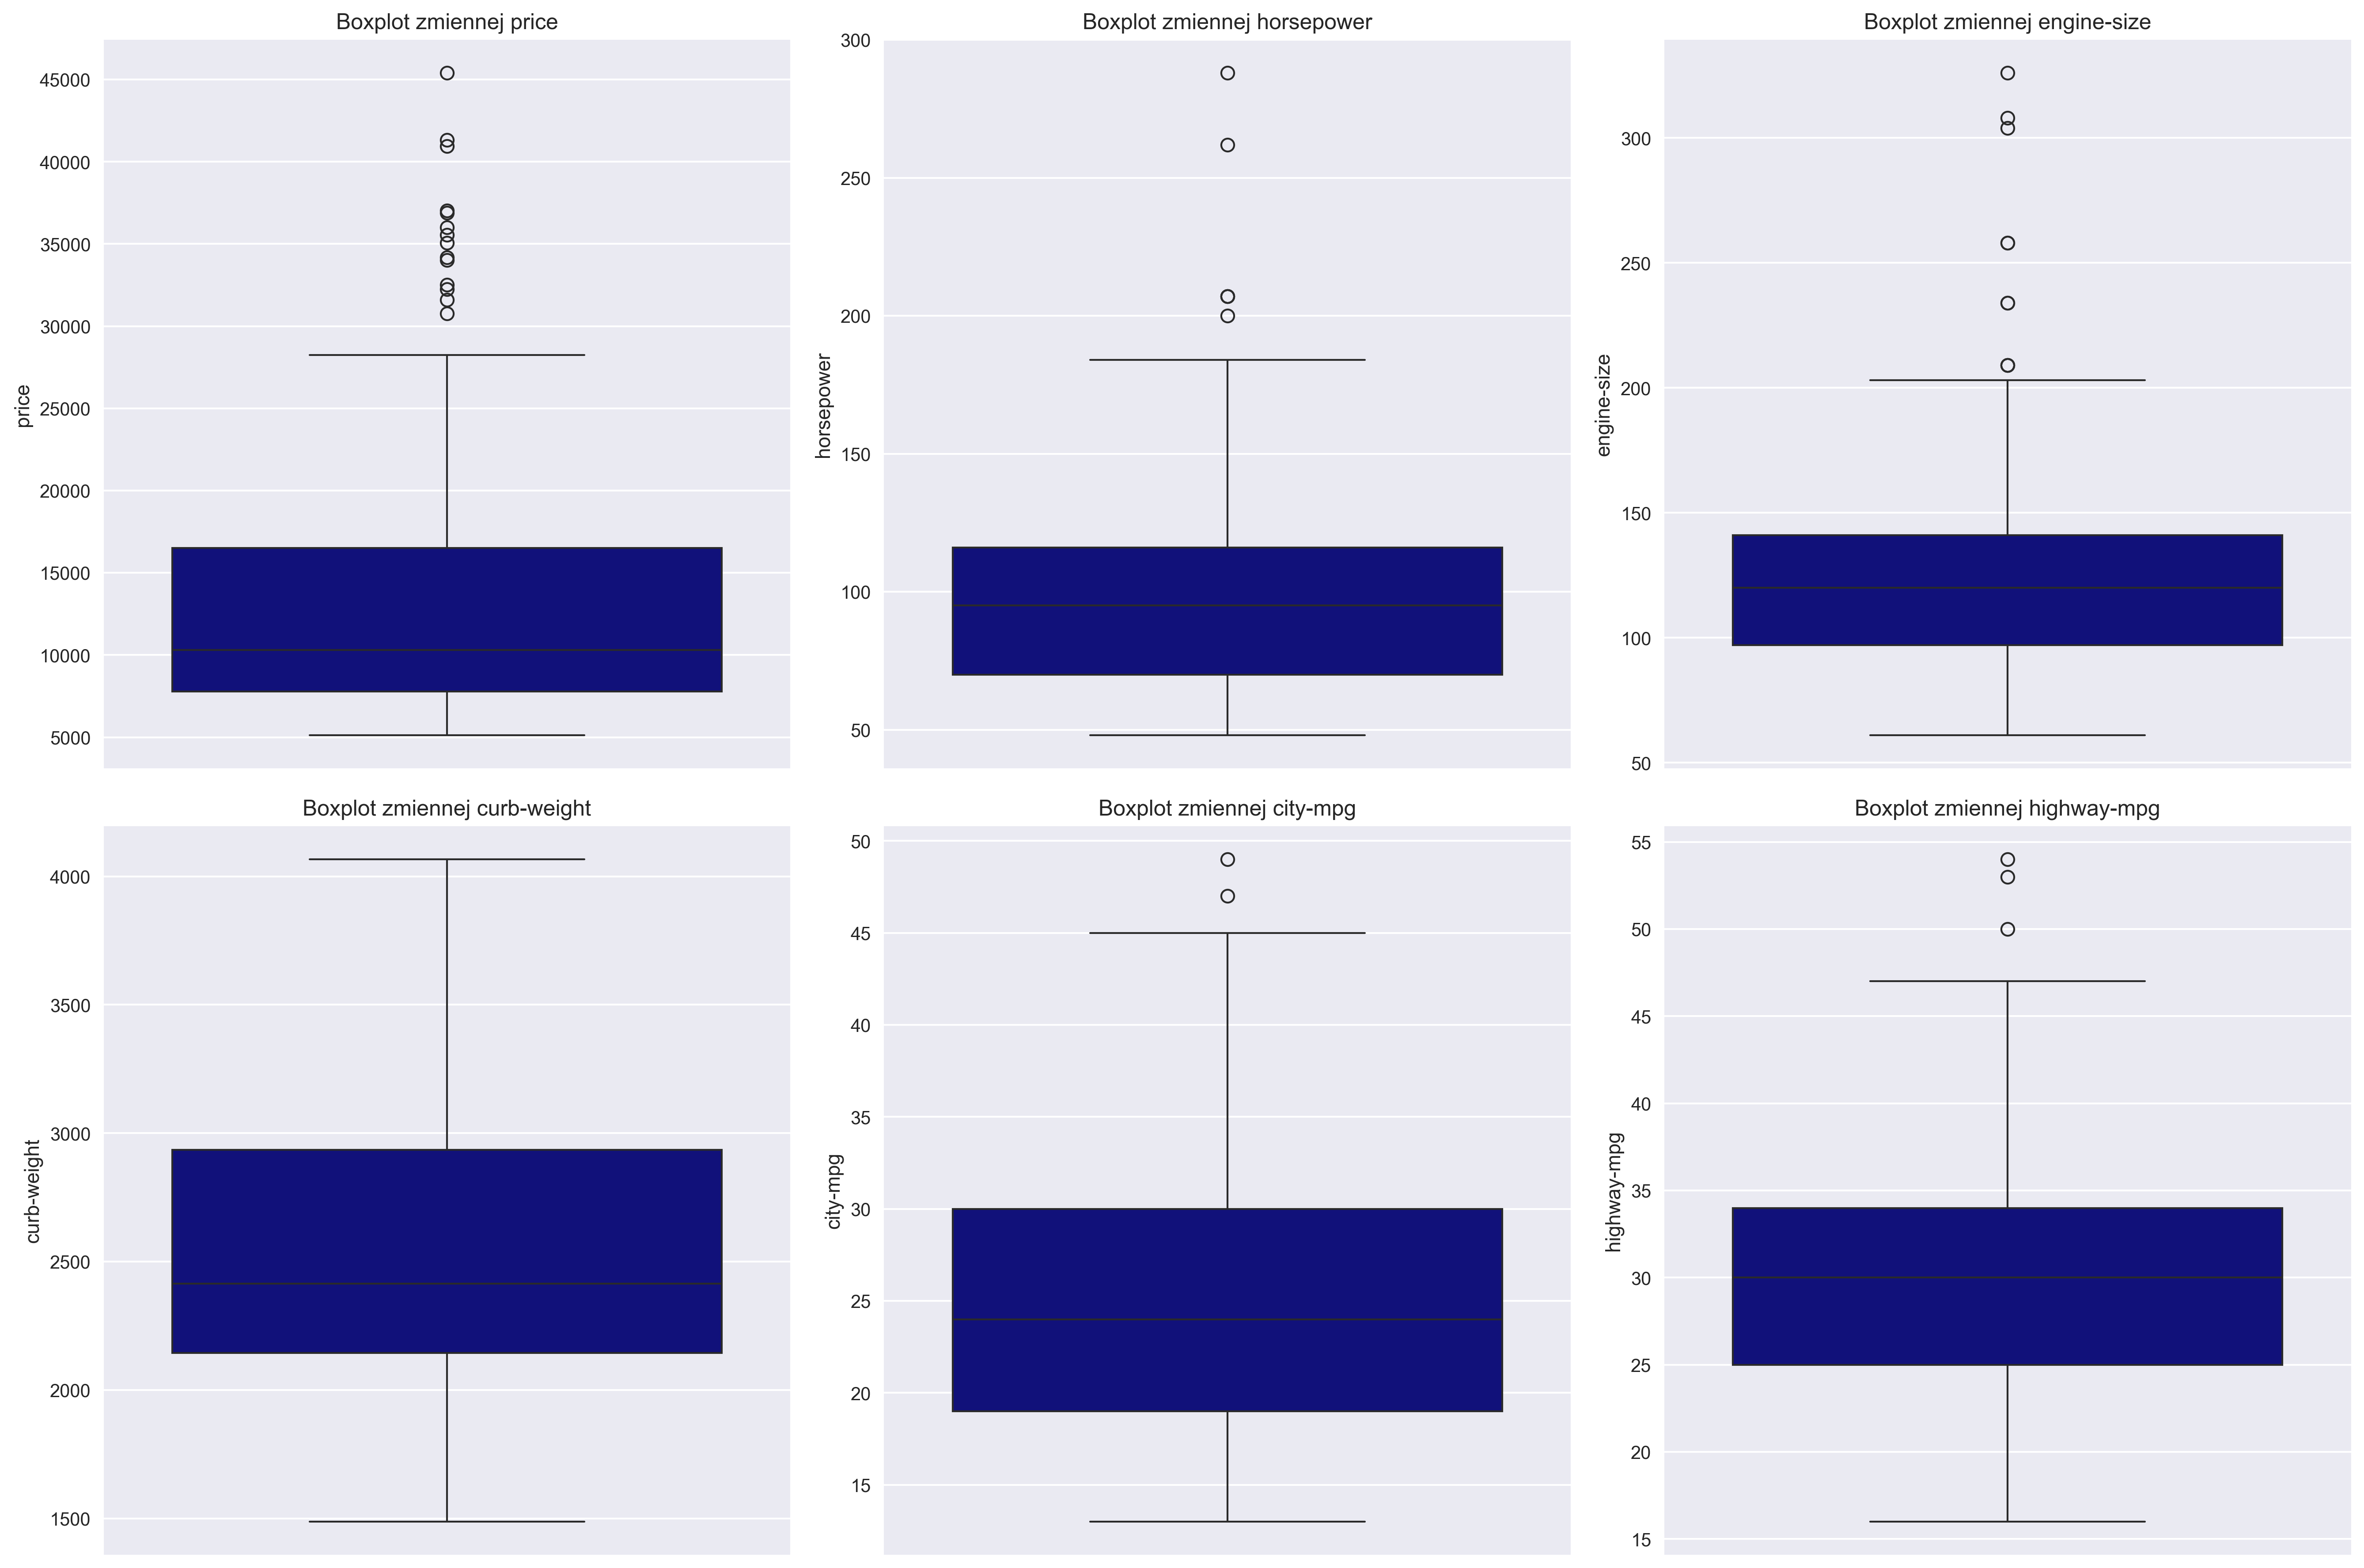
\includegraphics[width=0.9\textwidth]{figures/boxplots.png}
    \caption{Wykresy pudełkowe (boxploty) dla wybranych zmiennych}
    \label{fig:boxplots}
\end{figure}

Wykresy pudełkowe (Rys.~\ref{fig:boxplots}) przedstawiają kluczowe statystyki rozkładu: medianę, kwartyle, zakres oraz wartosci odstające. Widoczne są wartosci odstające w większosci zmiennych, szczególnie w przypadku `price`.

\begin{figure}[H]
    \centering
    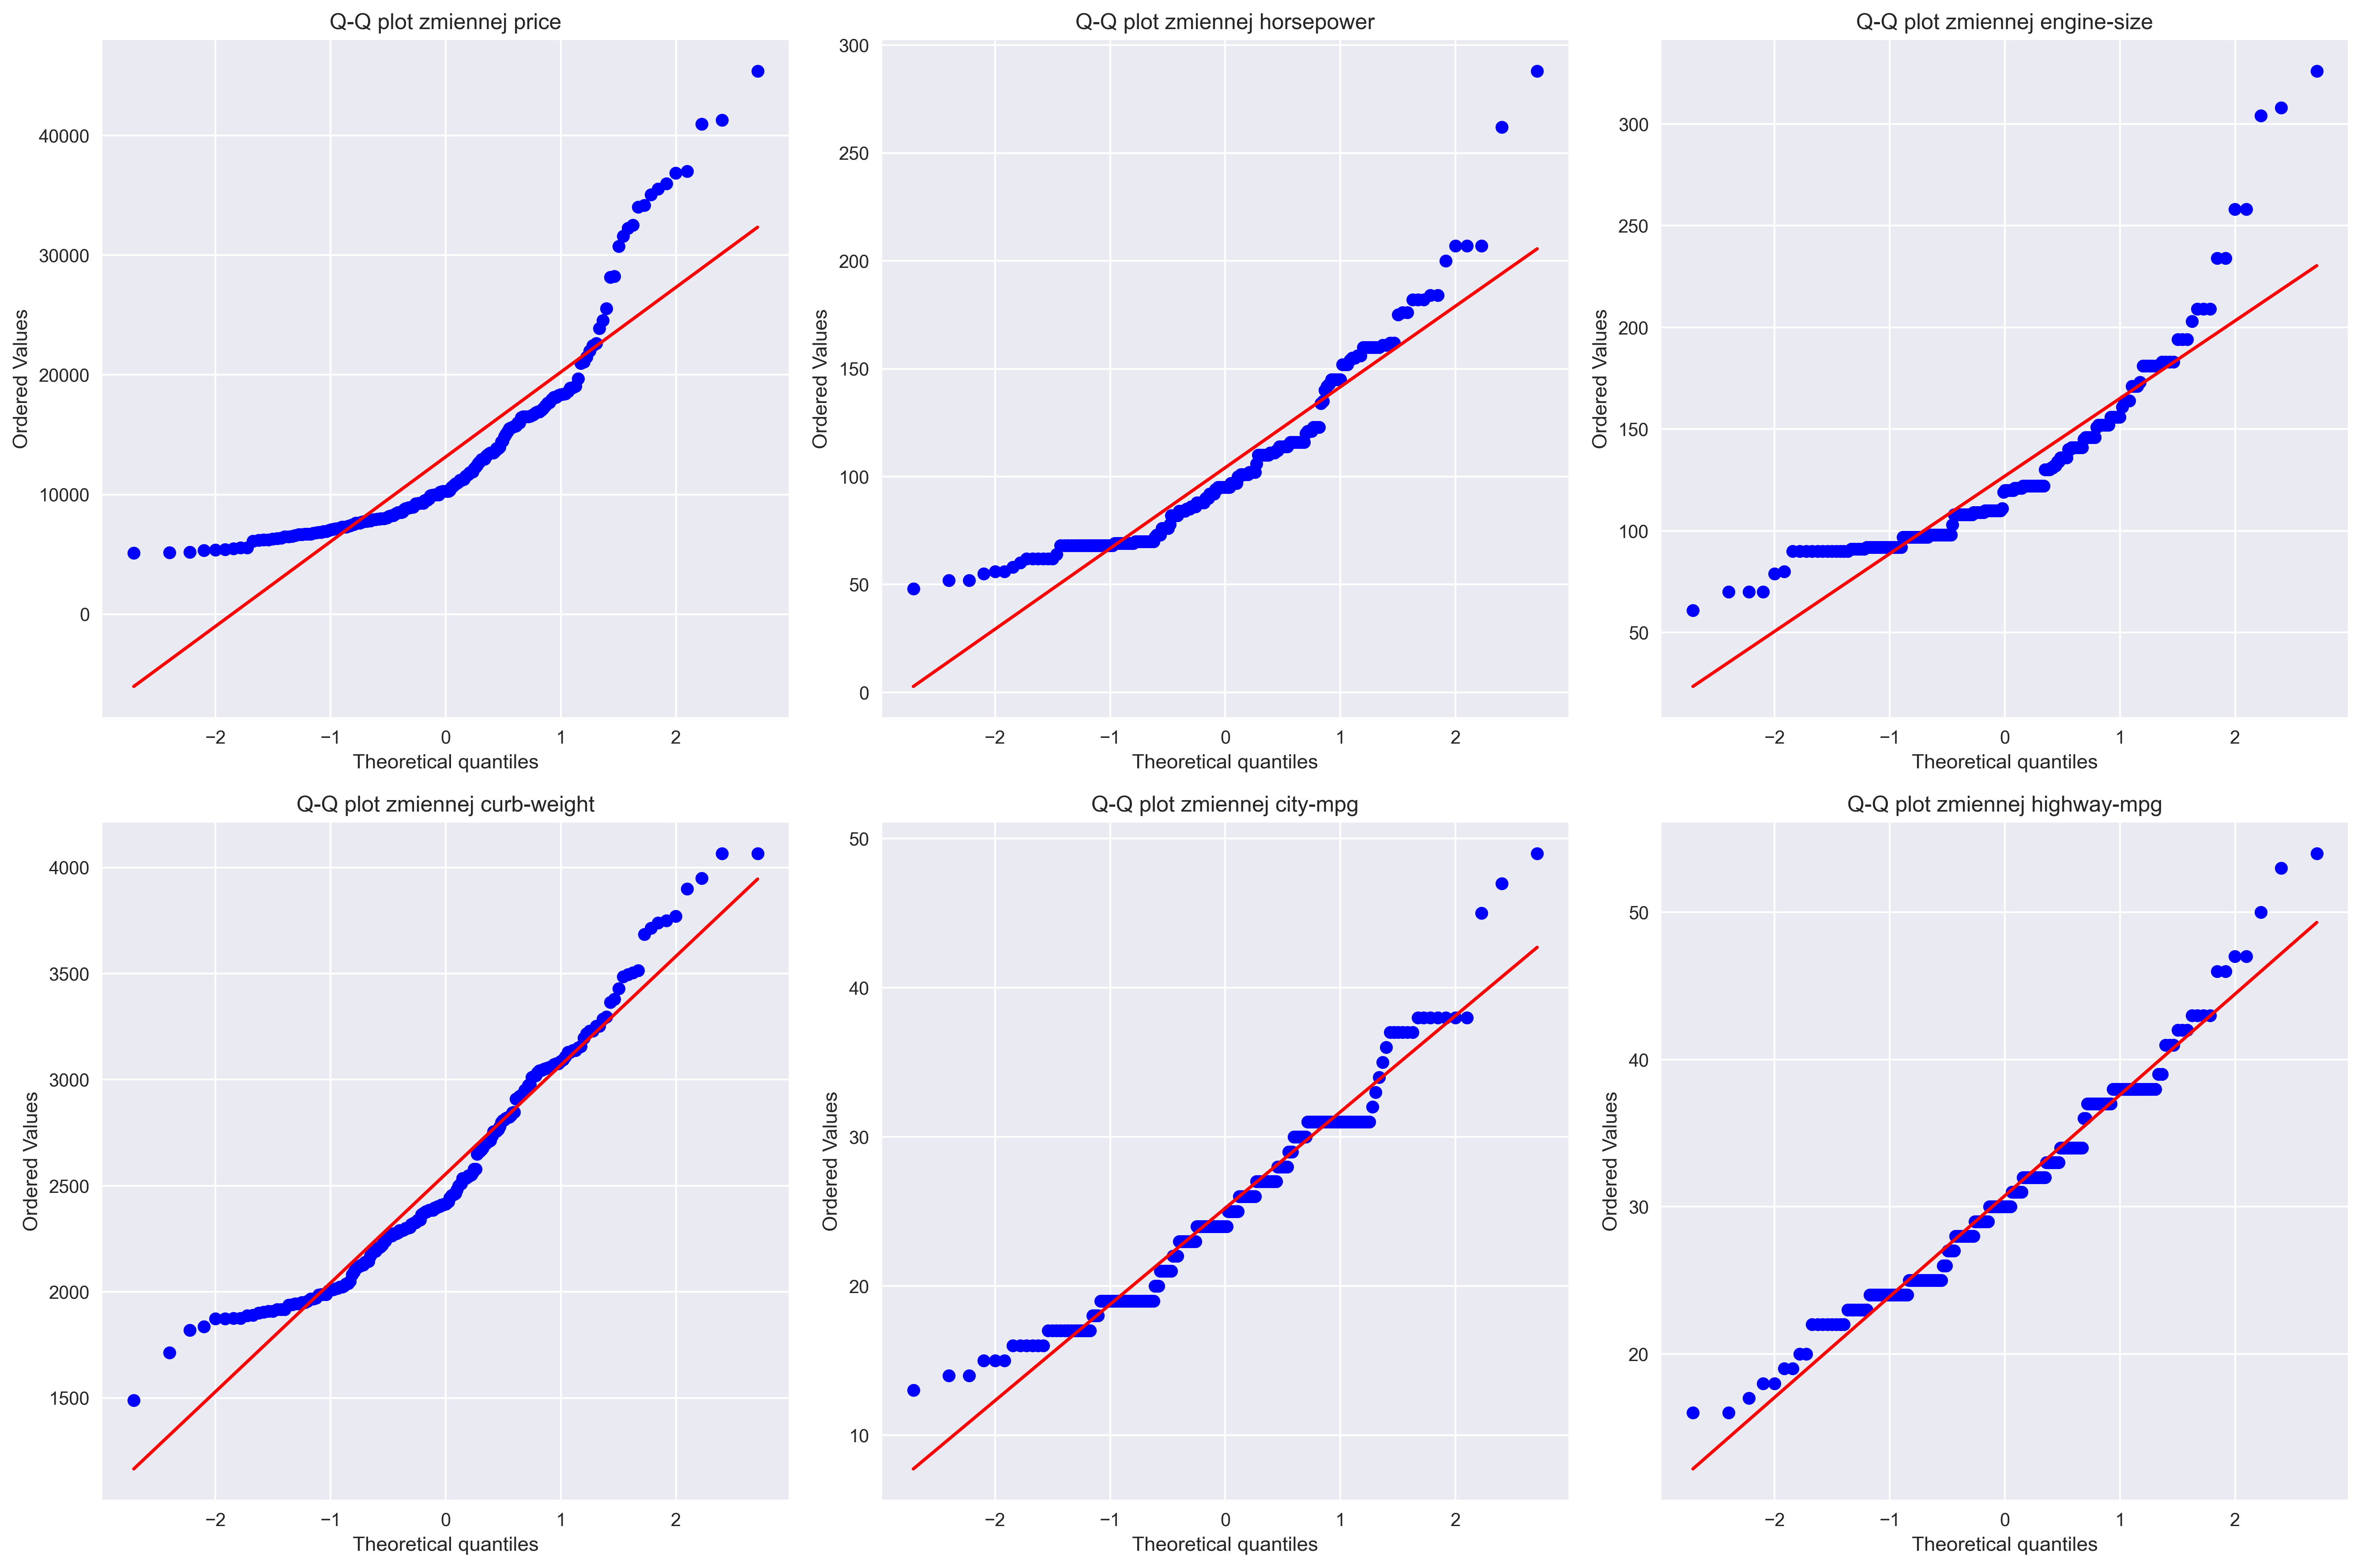
\includegraphics[width=0.9\textwidth]{figures/qq_plots.png}
    \caption{Wykresy kwantyl-kwantyl dla wybranych zmiennych}
    \label{fig:qq_plots}
\end{figure}

Wykresy kwantyl-kwantyl (Rys.~\ref{fig:qq_plots}) służą do oceny zgodnosci rozkładu empirycznego z rozkładem teoretycznym (w tym przypadku normalnym). Odchylenia punktów od linii prostej wskazują na odstępstwa od rozkładu normalnego.

\begin{figure}[H]
    \centering
    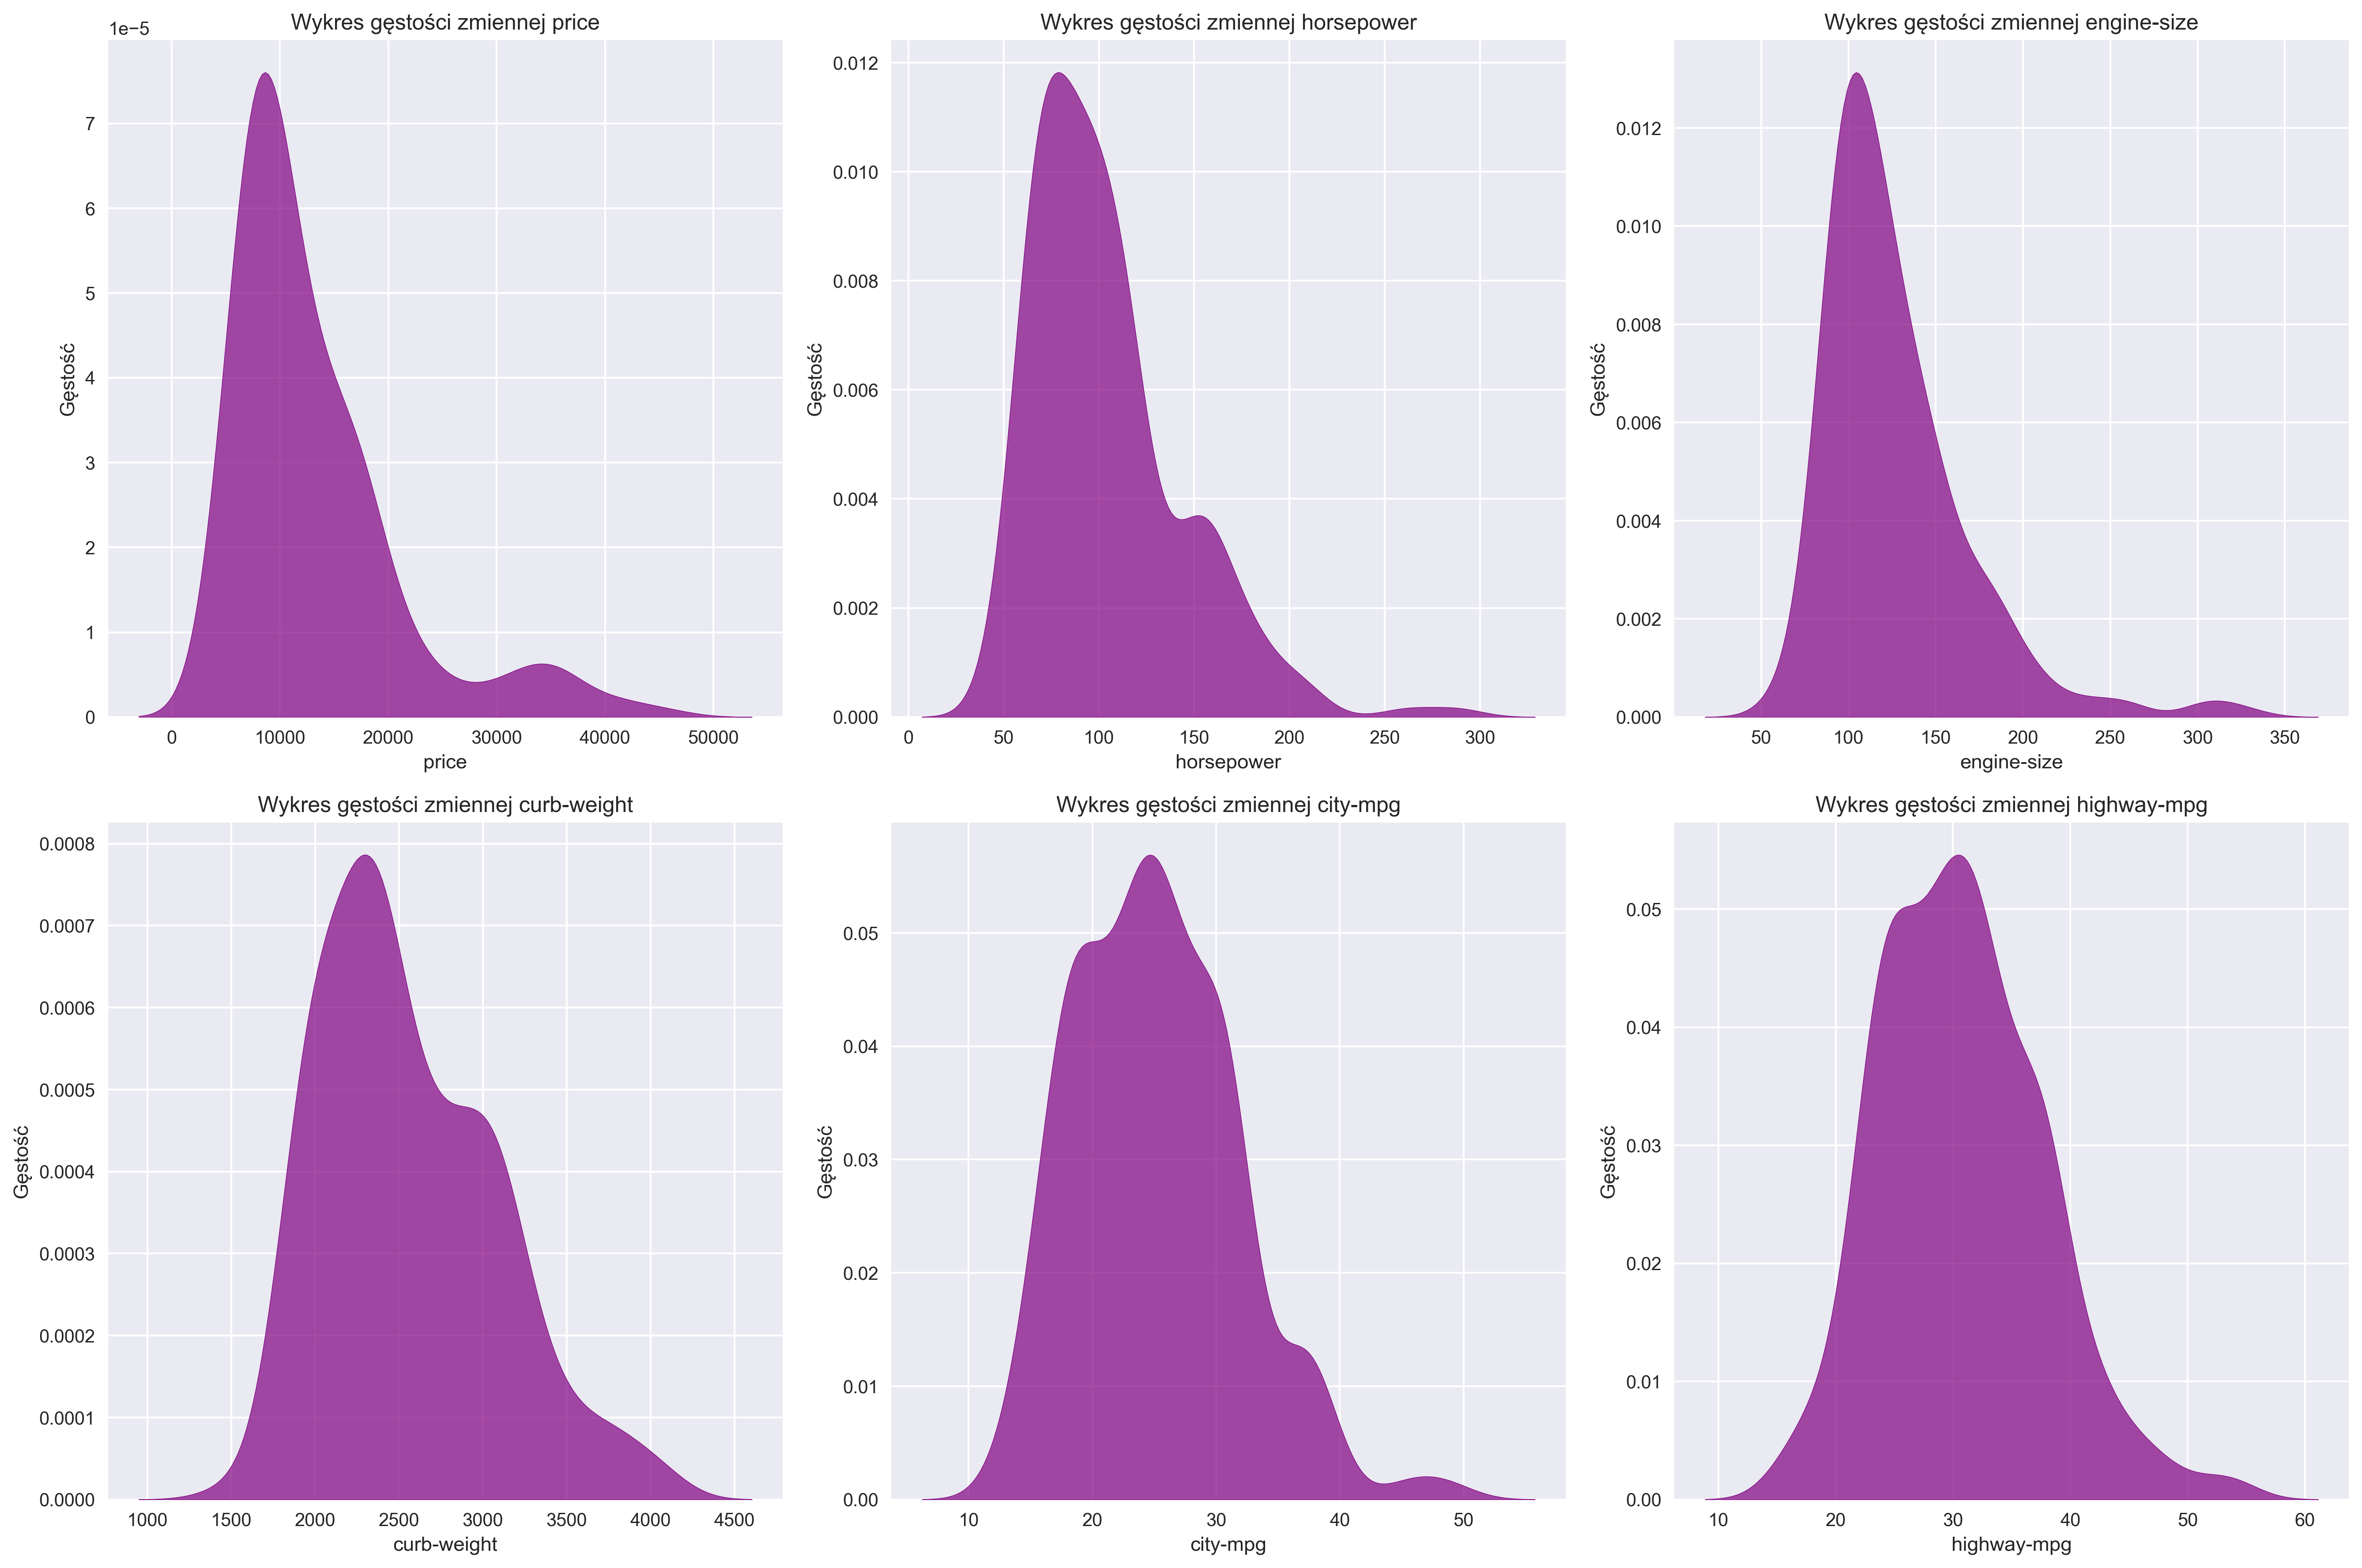
\includegraphics[width=0.9\textwidth]{figures/density_plots.png}
    \caption{Wykresy gęstosci prawdopodobieństwa dla wybranych zmiennych}
    \label{fig:density_plots}
\end{figure}

Wykresy gęstosci (Rys.~\ref{fig:density_plots}) wizualizują ciągły rozkład prawdopodobieństwa badanych zmiennych. Wyraźnie widoczne są wielomodalne rozkłady dla niektórych zmiennych.

\begin{figure}[H]
    \centering
    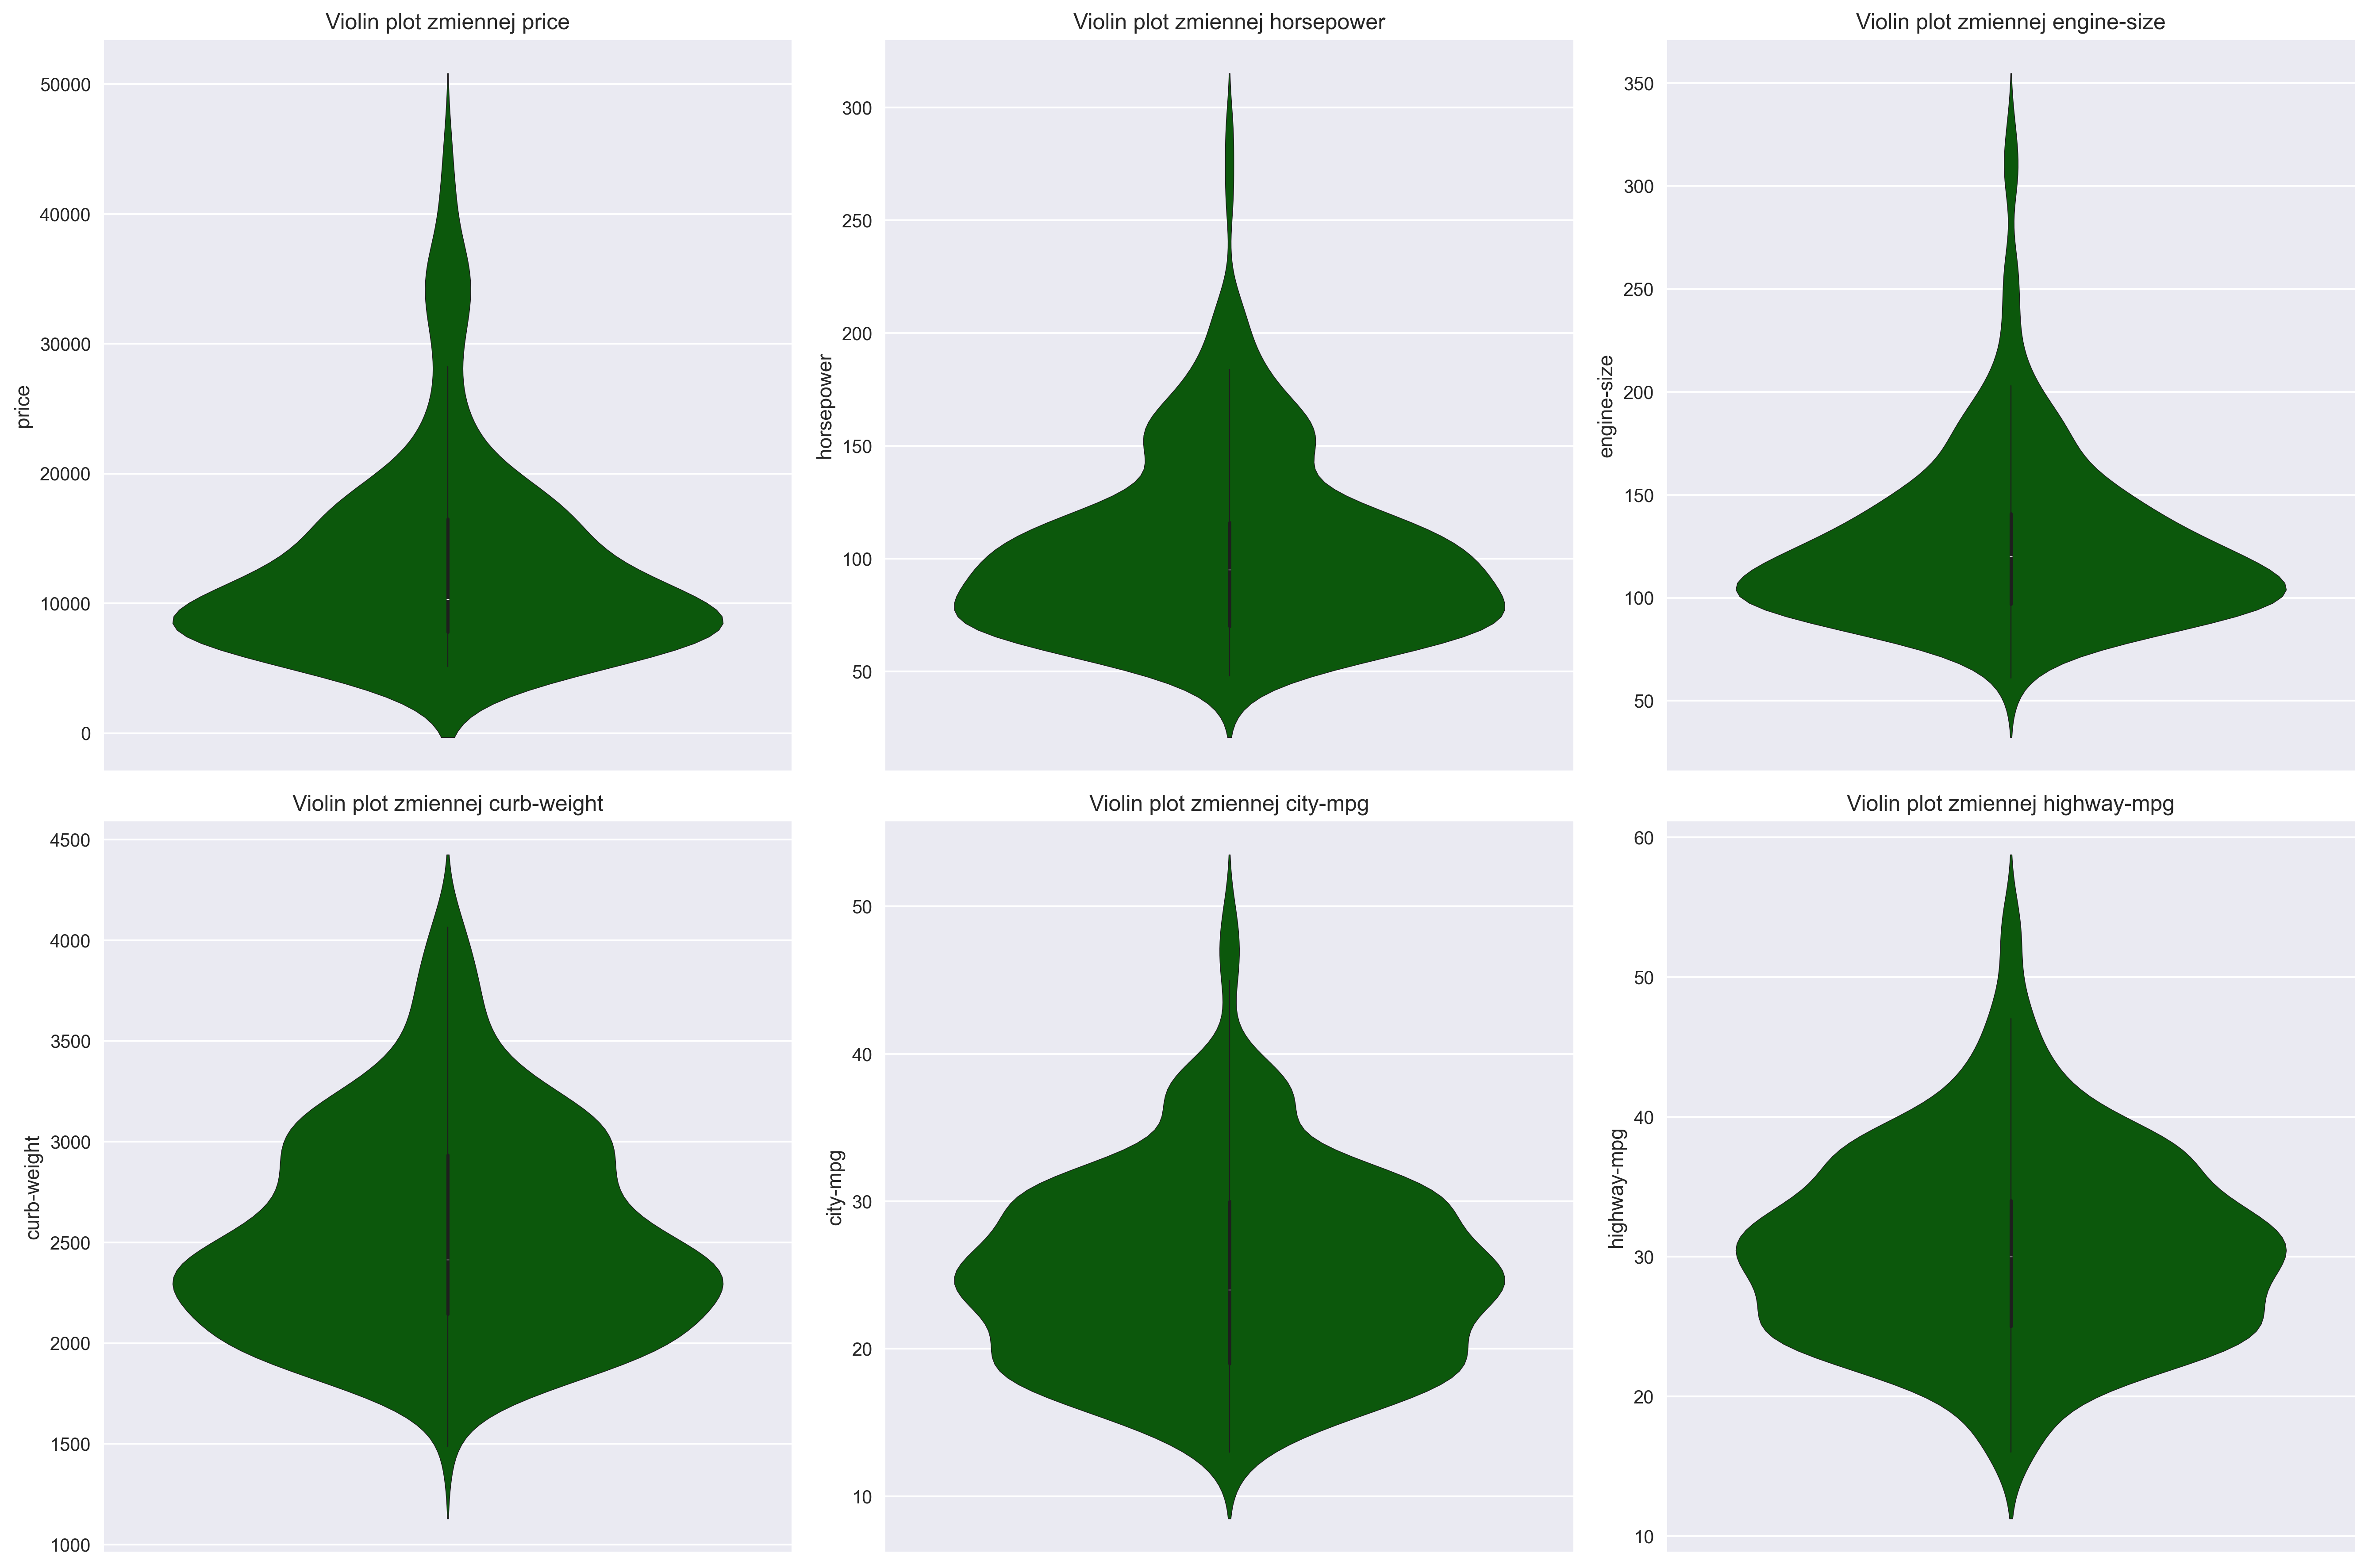
\includegraphics[width=0.9\textwidth]{figures/violin_plots.png}
    \caption{Wykresy skrzypcowe dla wybranych zmiennych}
    \label{fig:violin_plots}
\end{figure}

Wykresy skrzypcowe (Rys.~\ref{fig:violin_plots}) łączą cechy boxplotów i wykresów gęstosci, pokazując zarówno podstawowe statystyki, jak i kształt rozkładu.

\begin{figure}[H]
    \centering
    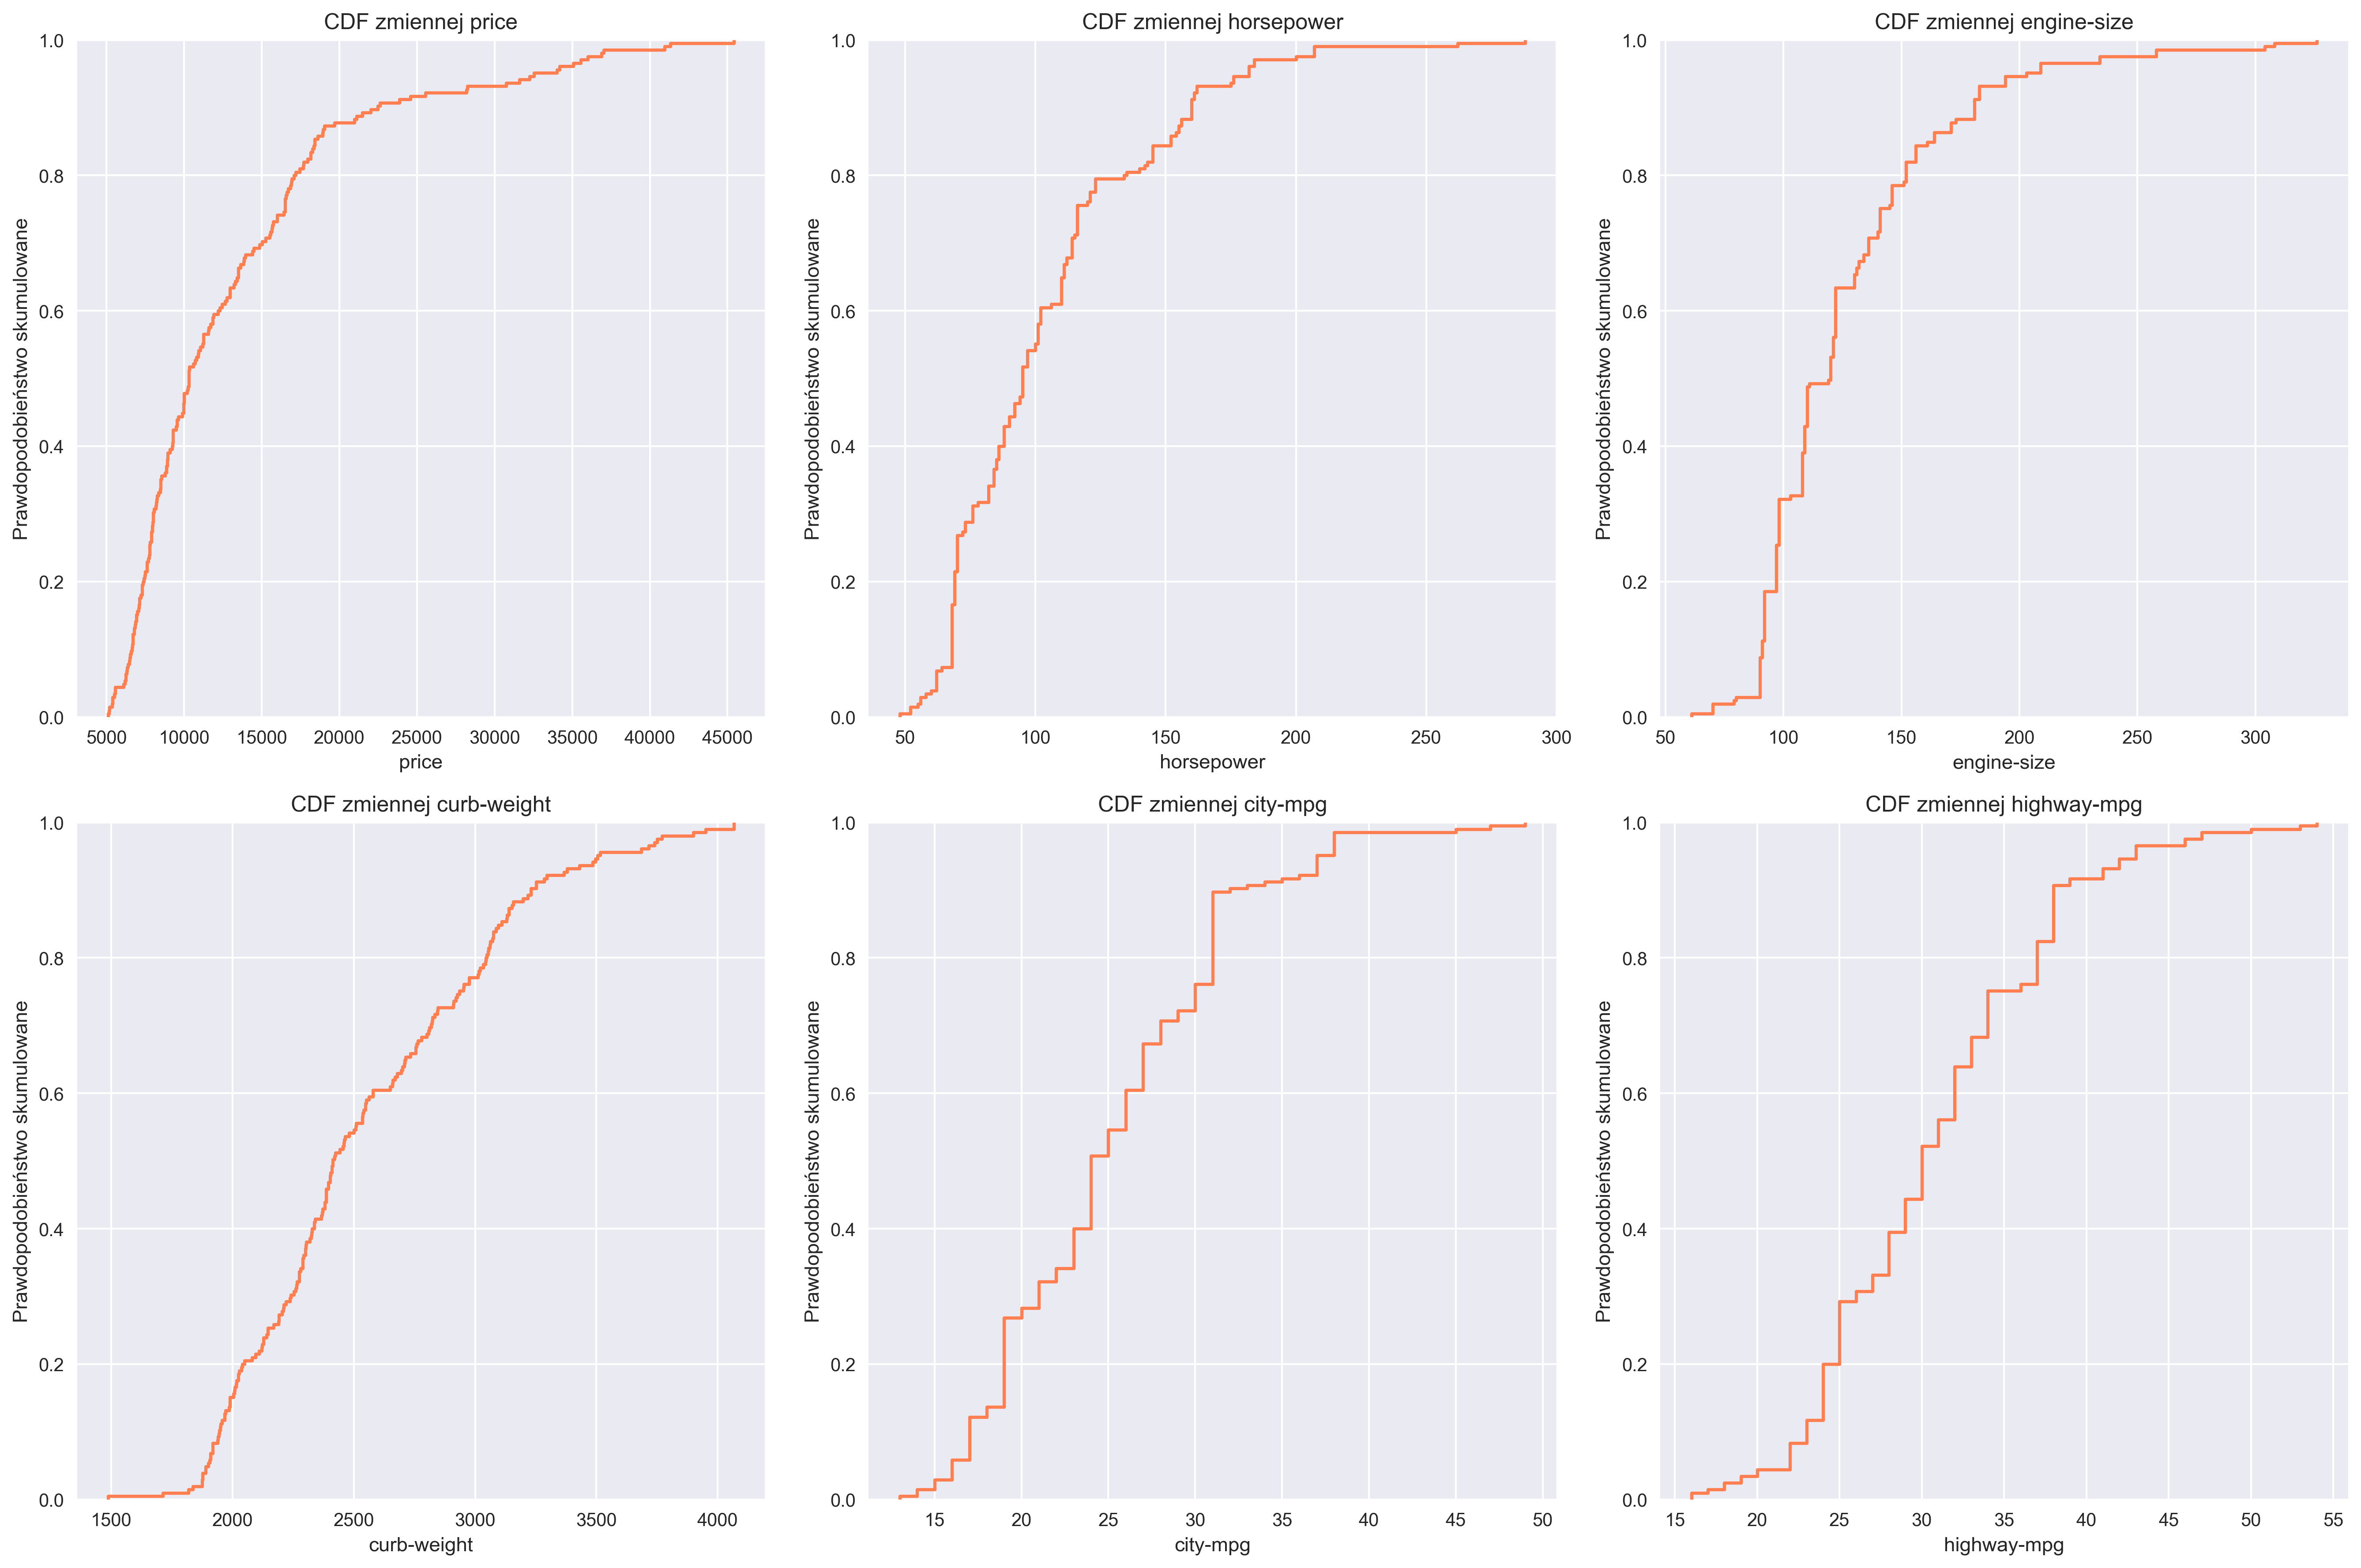
\includegraphics[width=0.9\textwidth]{figures/cdf_plots.png}
    \caption{Empiryczne dystrybuanty dla wybranych zmiennych}
    \label{fig:cdf_plots}
\end{figure}

Empiryczne dystrybuanty (Rys.~\ref{fig:cdf_plots}) przedstawiają funkcje rozkładu skumulowanego, które są szczególnie użyteczne do analizy kwantyli i porównywania rozkładów.

\begin{figure}[H]
    \centering
    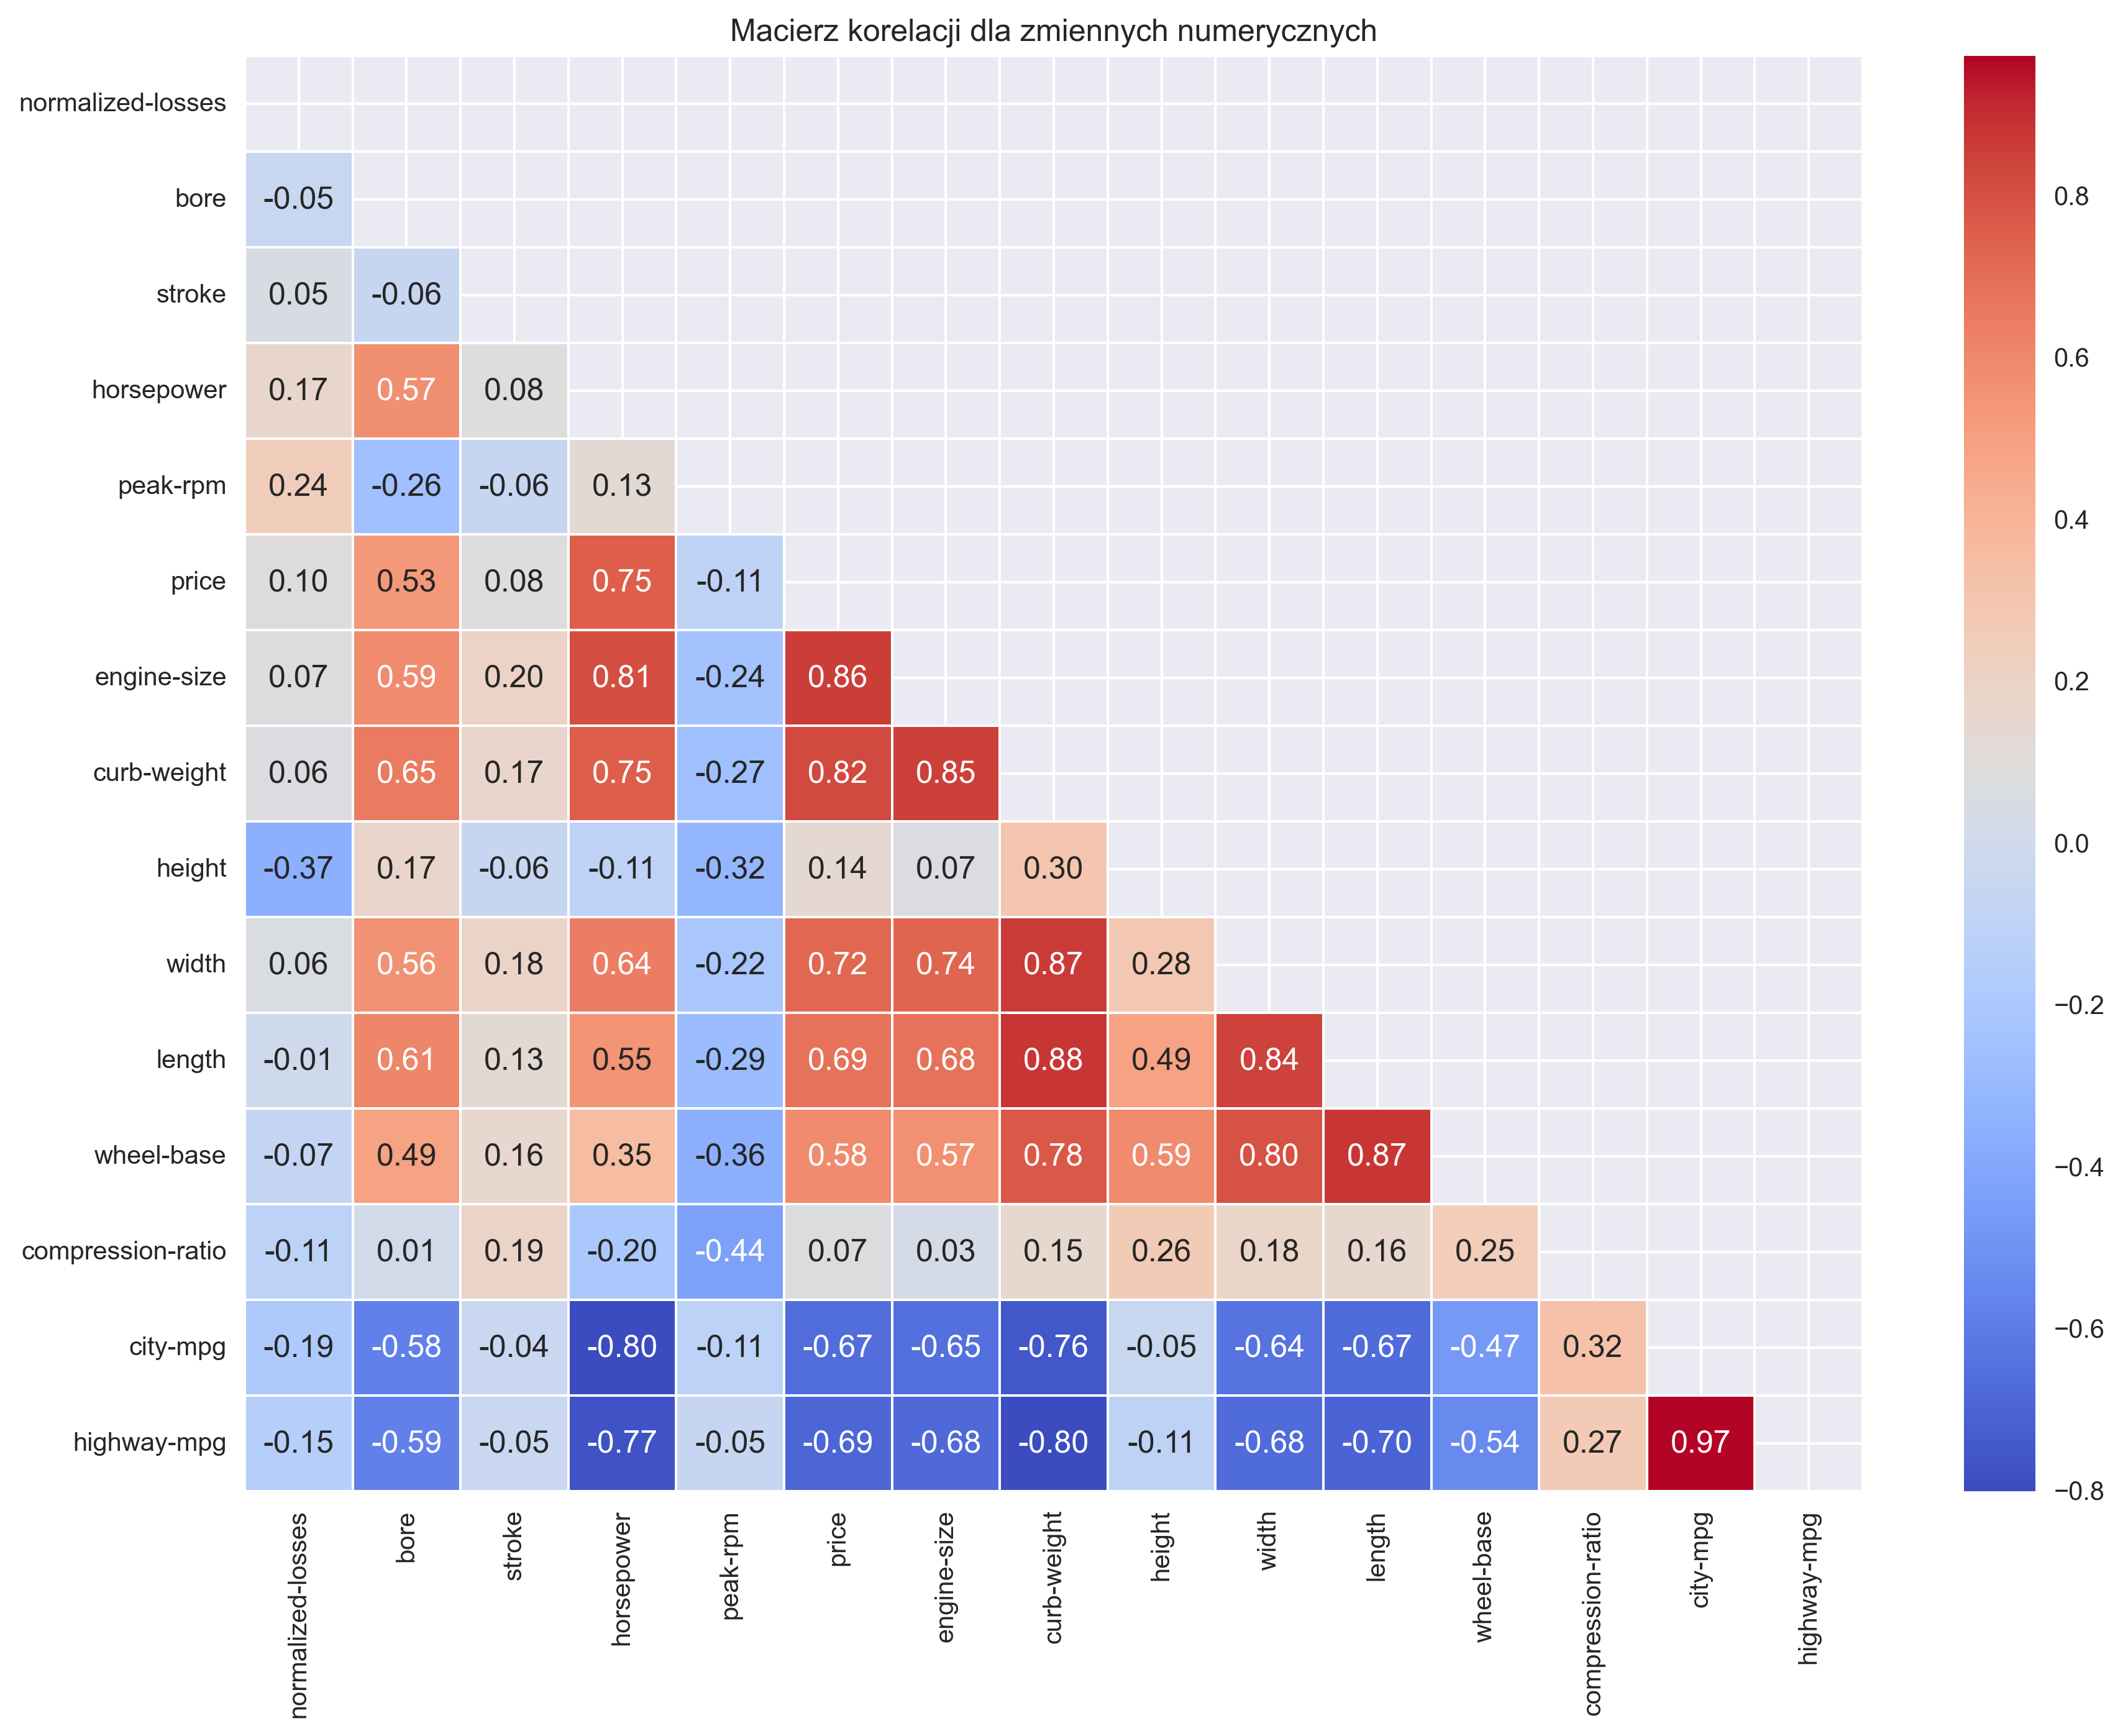
\includegraphics[width=0.9\textwidth]{figures/correlation_heatmap.png}
    \caption{Macierz korelacji dla zmiennych numerycznych}
    \label{fig:correlation_heatmap}
\end{figure}

Macierz korelacji (Rys.~\ref{fig:correlation_heatmap}) uwidacznia silne zależnosci między niektórymi zmiennymi, na przykład korelację ujemną między `city-mpg` a `engine-size` oraz silną dodatnią korelację między `length` a `width`.

\begin{figure}[H]
    \centering
    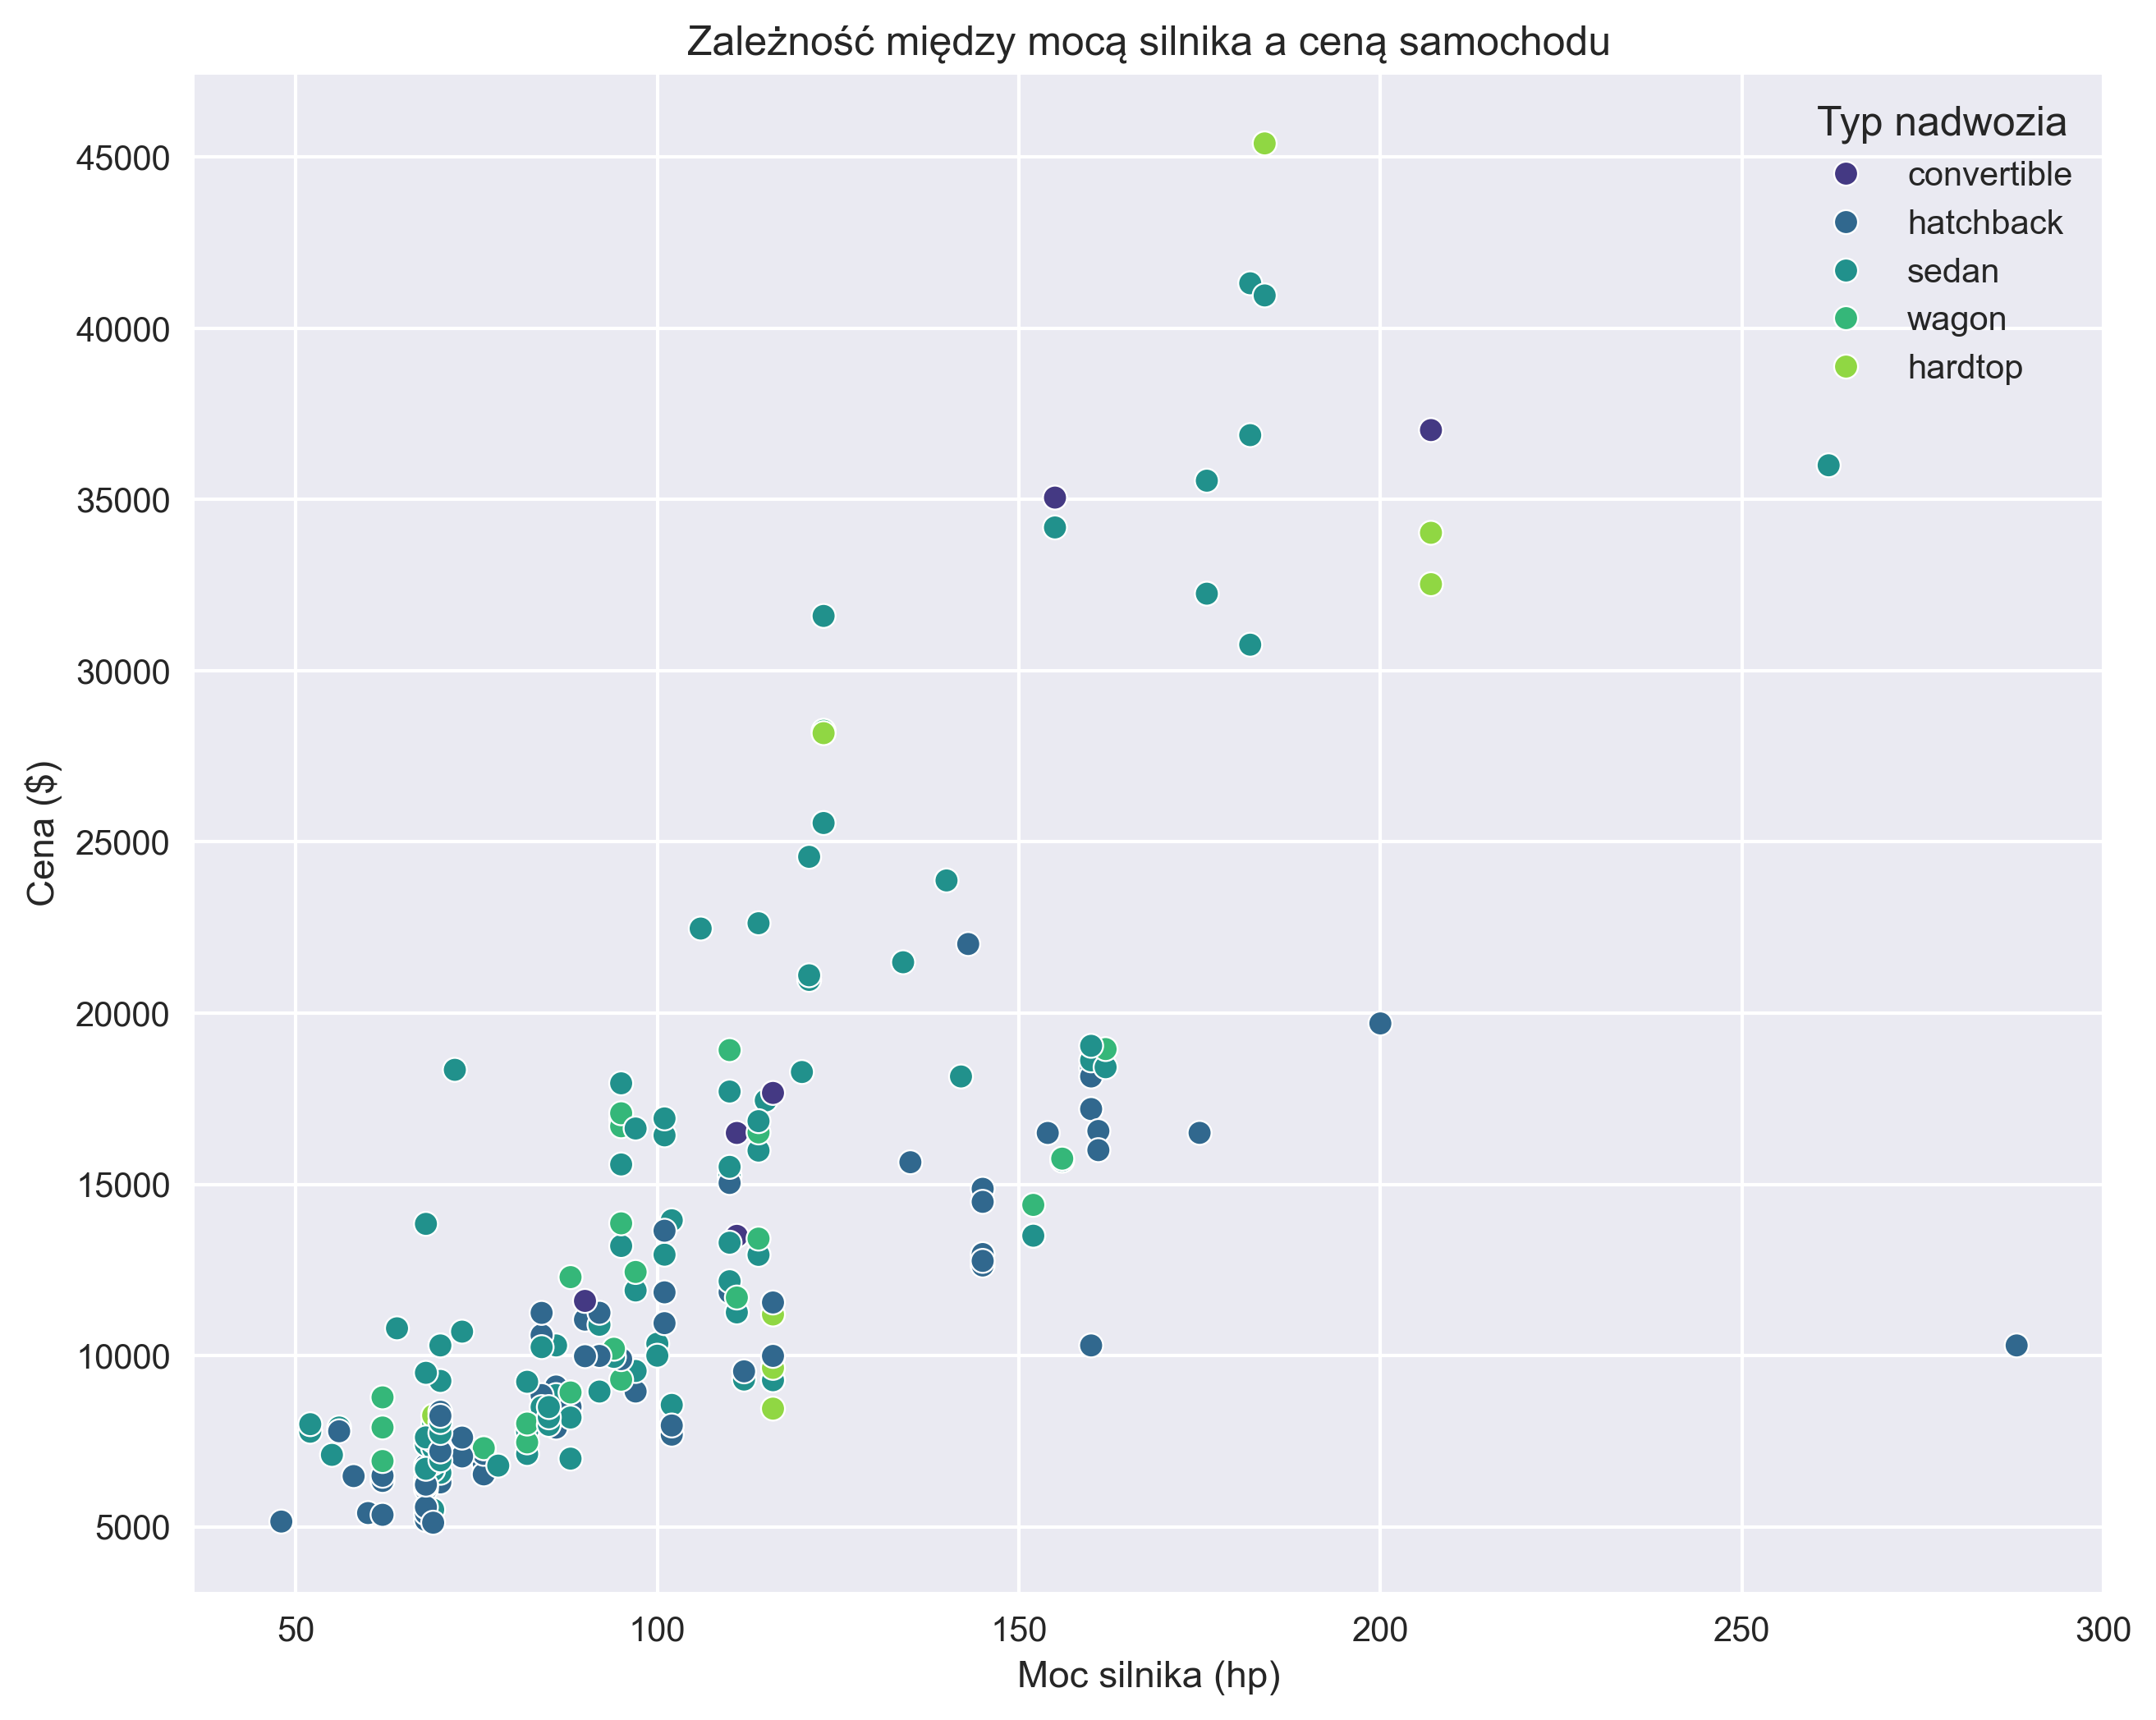
\includegraphics[width=0.85\textwidth]{figures/scatter_horsepower_price.png}
    \caption{Wykres rozrzutu: zależnosc między mocą silnika a ceną z rozróżnieniem typu nadwozia}
    \label{fig:scatter_horsepower_price}
\end{figure}

Wykres rozrzutu (Rys.~\ref{fig:scatter_horsepower_price}) pokazuje pozytywną zależnosc między mocą silnika a ceną samochodu, z rozróżnieniem typów nadwozia. Widoczne jest, że samochody sportowe (`convertible`) i sedan mają tendencję do wyższych cen przy podobnej mocy.

\begin{figure}[H]
    \centering
    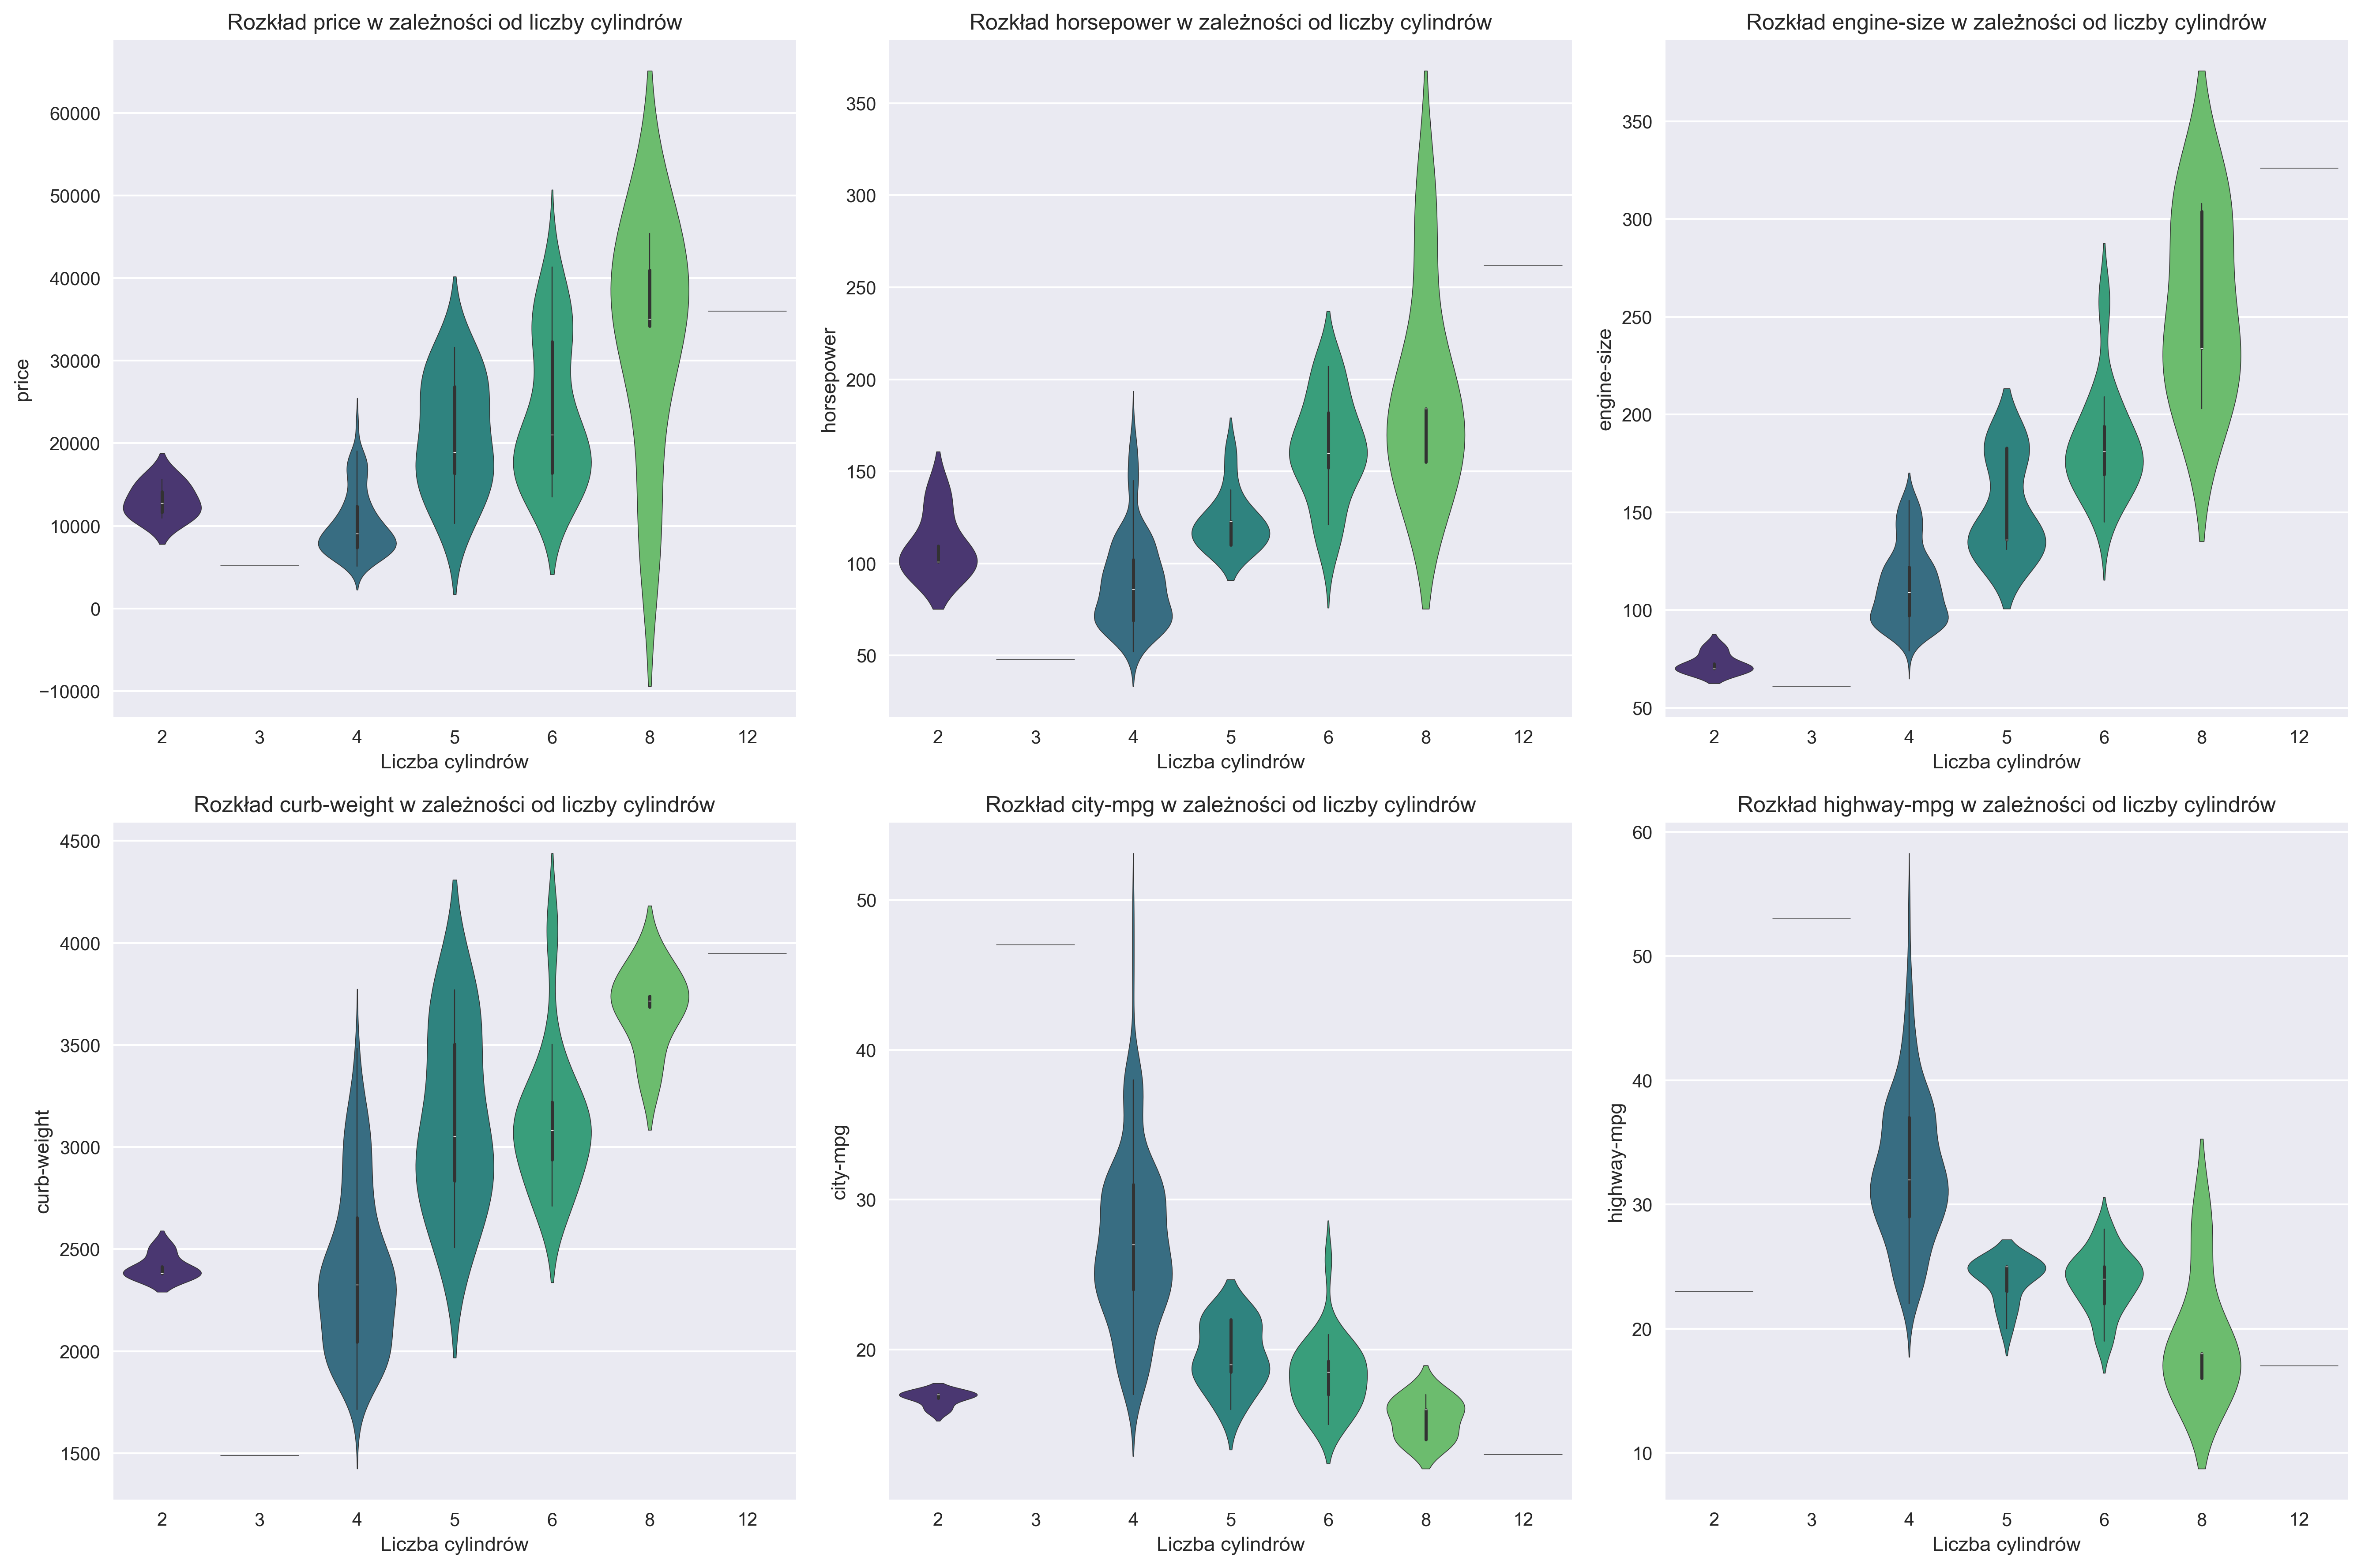
\includegraphics[width=0.9\textwidth]{figures/violin_by_cylinders.png}
    \caption{Wykresy skrzypcowe w zależnosci od liczby cylindrów}
    \label{fig:violin_by_cylinders}
\end{figure}

Wykresy skrzypcowe według liczby cylindrów (Rys.~\ref{fig:violin_by_cylinders}) ukazują, jak rozkłady zmiennych zależą od liczby cylindrów silnika. Widoczny jest trend rosnący dla mocy silnika (`horsepower`) i pojemnosci silnika (`engine-size`) wraz ze wzrostem liczby cylindrów.

\section{Sprawdzenie normalnosci rozkładów danych}

Aby ocenic, czy zmienne numeryczne w zbiorze danych Automobile pochodzą z rozkładu normalnego, przeprowadzono trzy różne testy statystyczne:
\begin{itemize}
    \item Test Shapiro-Wilka
    \item Test D'Agostino-Pearsona
    \item Test Andersona-Darlinga
\end{itemize}

Każdy z testów ocenia normalnosc rozkładu w nieco inny sposób, co pozwala na bardziej kompleksową analizę.

\begin{figure}[H]
    \centering
    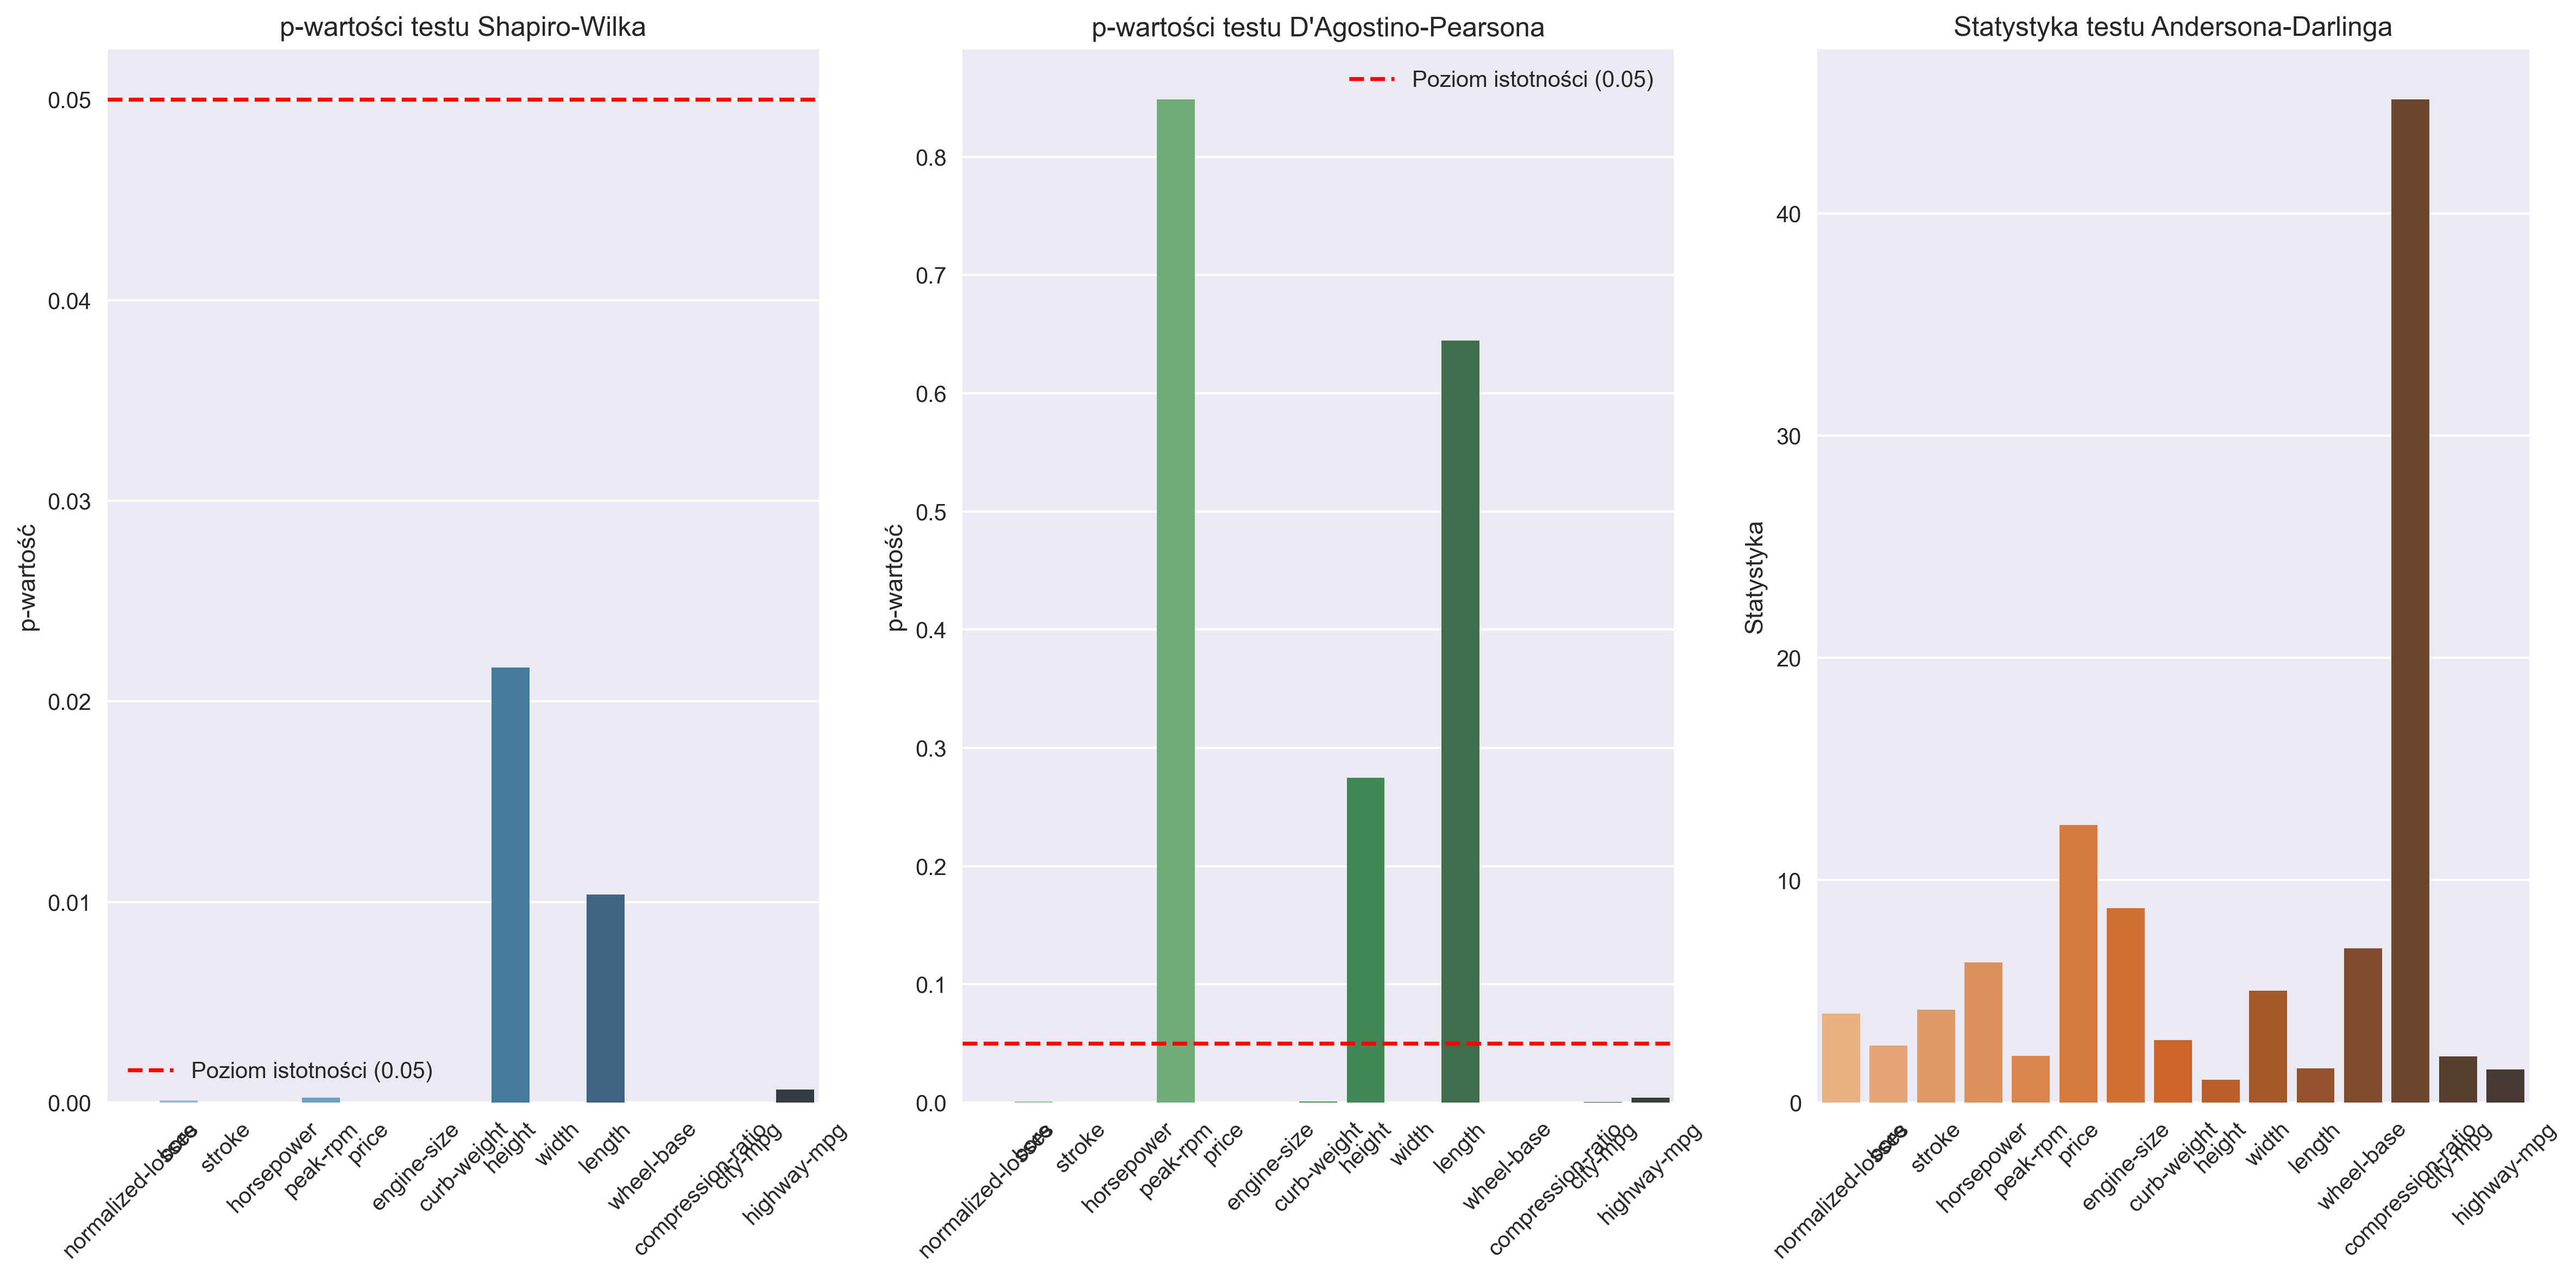
\includegraphics[width=0.9\textwidth]{figures/normality_tests.png}
    \caption{Wyniki testów normalnosci dla zmiennych ciągłych}
    \label{fig:normality_tests}
\end{figure}

\subsection{Test Shapiro-Wilka}

Wyniki testu przedstawione zostały na lewym wykresie Rys.~\ref{fig:normality_tests}. 

\textbf{Wnioski:}

Dla żadnej z badanych zmiennych \textbf{p-wartosc nie przekroczyła poziomu istotnosci 0.05}, co oznacza, że dla wszystkich zmiennych \textbf{odrzucamy hipotezę o normalnosci rozkładu}. Zmienna \texttt{curb-weight} osiągnęła najwyższą p-wartosc (~0.023), jednak nadal poniżej progu istotnosci.

\subsection{Test D'Agostino-Pearsona}

Ten test łączy informację o skosnosci i kurtozie w celu oceny normalnosci (srodkowy wykres na Rys.~\ref{fig:normality_tests}).

\textbf{Wnioski:}

\textbf{Tylko dwie zmienne (\texttt{horsepower} i \texttt{width}) mają p-wartosc wyraźnie przekraczającą 0.05}, co oznacza brak podstaw do odrzucenia hipotezy o normalnosci. Pozostałe zmienne nie spełniają założenia normalnosci, podobnie jak w tescie Shapiro-Wilka.

\subsection{Test Andersona-Darlinga}

Na ostatnim wykresie Rys.~\ref{fig:normality_tests} przedstawiono wartosci statystyki testowej. Im wyższa wartosc, tym większe odchylenie od rozkładu normalnego.

\textbf{Wnioski:}

Zmienna \texttt{compression-ratio} wyróżnia się \textbf{najwyższą statystyką testu (~45)}, co wskazuje na \textbf{znaczne odstępstwo od rozkładu normalnego}. Najniższe wartosci statystyki występują m.in. dla \texttt{height}, \texttt{curb-weight} i \texttt{engine-size}.

\begin{figure}[H]
    \centering
    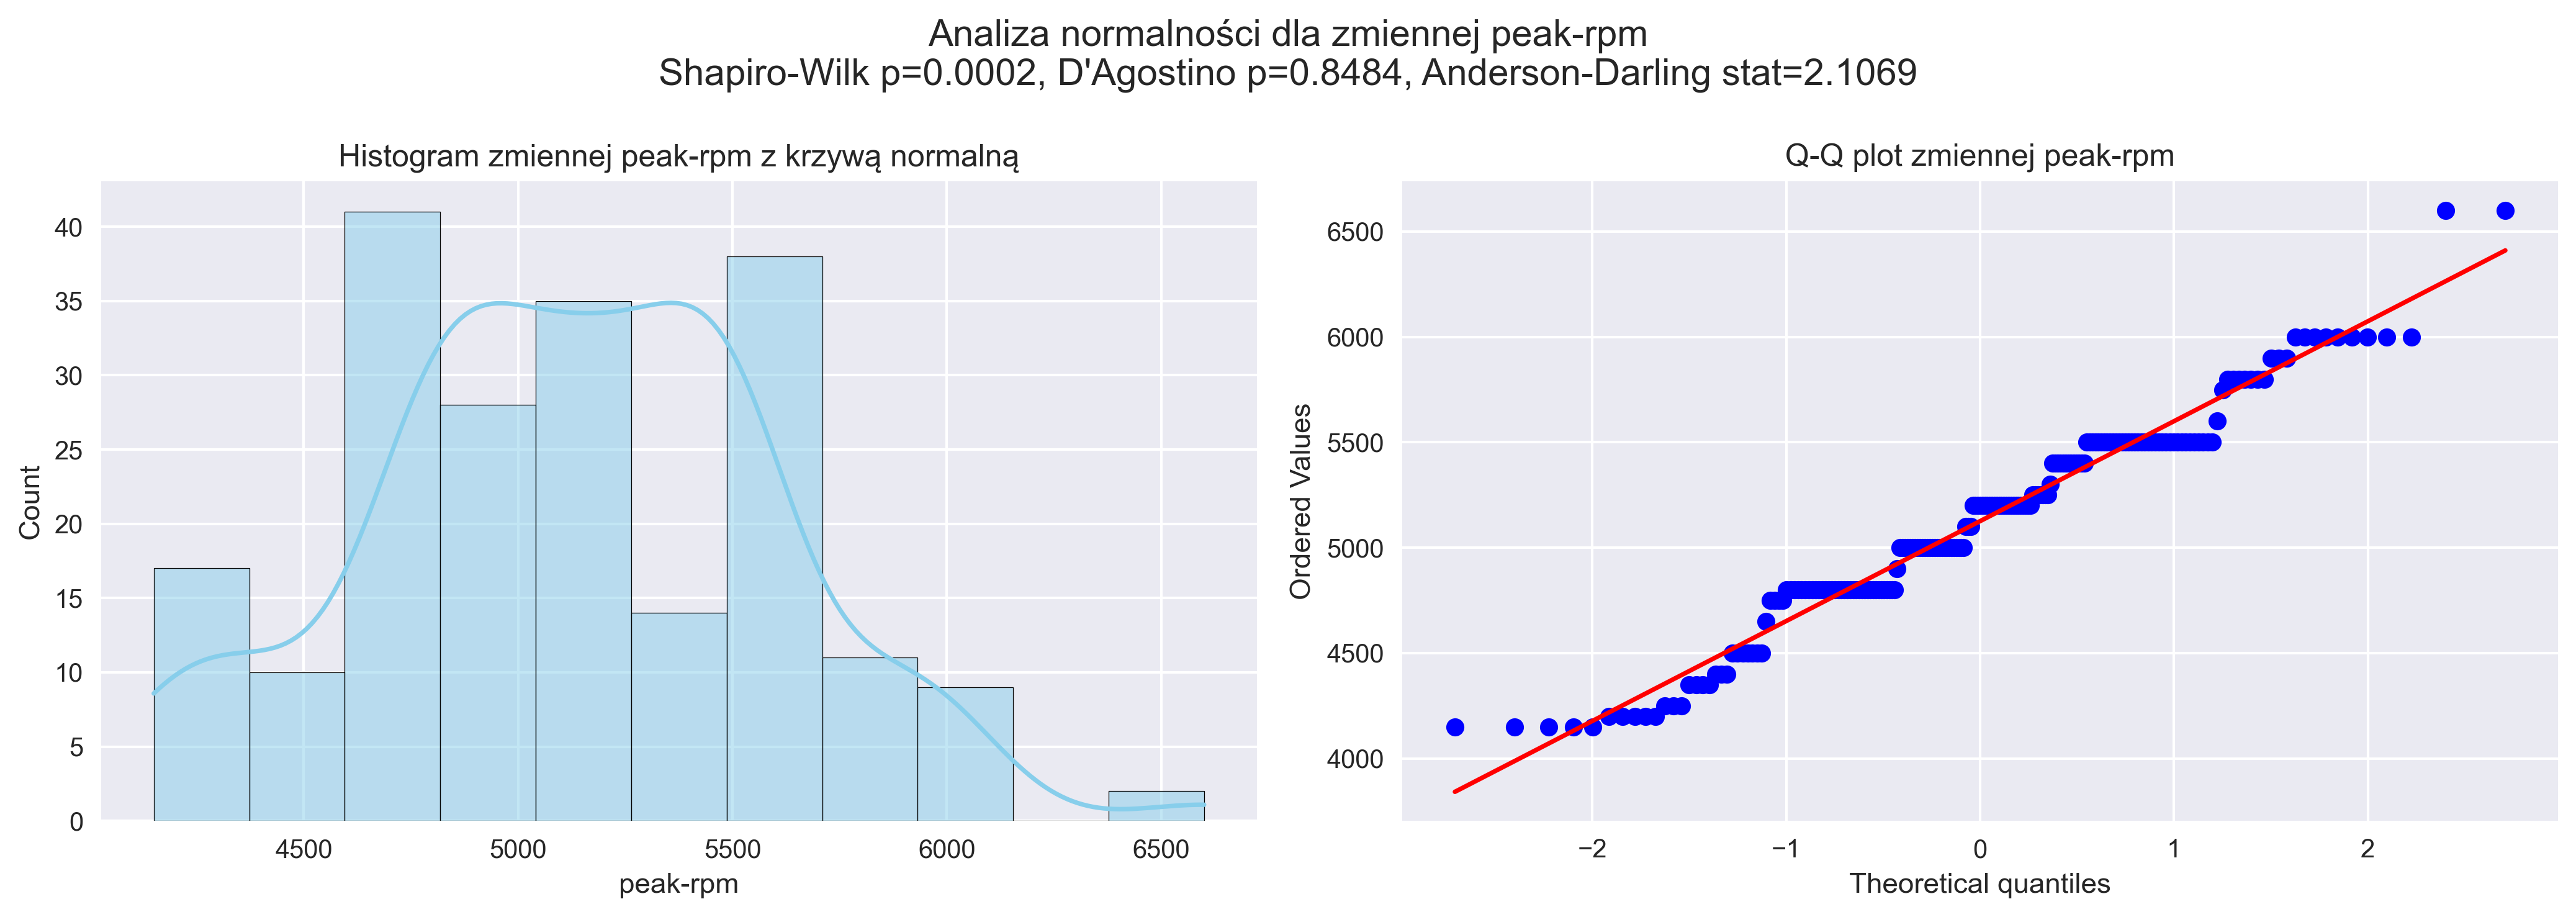
\includegraphics[width=0.9\textwidth]{figures/normality_detail_peak_rpm.png}
    \caption{Szczegółowa analiza normalnosci dla zmiennej peak_rpm}
    \label{fig:normality_detail_horsepower}
\end{figure}

Analiza szczegółowa dla zmiennej \texttt{peak_rpm} (Rys.~\ref{fig:normality_detail_peak_rpm}) potwierdza jej względną bliskosc do rozkładu normalnego, choc nadal widoczne są pewne odstępstwa.

\subsection{Podsumowanie}

Na podstawie przeprowadzonych testów można stwierdzic, że:

\begin{itemize}
    \item \textbf{Większosc zmiennych w zbiorze danych nie pochodzi z rozkładu normalnego}.
    \item Tylko nieliczne cechy (np. \texttt{horsepower}, \texttt{width}) mogą byc rozpatrywane jako zbliżone do rozkładu normalnego.
    \item Przed użyciem metod statystycznych zakładających normalnosc (np. testy parametryczne, PCA) \textbf{zaleca się przeprowadzenie transformacji danych}, np. transformacji logarytmicznej lub standaryzacji.
\end{itemize}

Dzięki zastosowaniu trzech różnych testów uzyskano spójną i wiarygodną ocenę rozkładów cech numerycznych.

\subsection{Kod implementujący testy normalnosci}
\begin{lstlisting}[language=Python, caption=Kod testów normalnosci]
import matplotlib.pyplot as plt
import seaborn as sns
from scipy import stats
import os

# Ensure figures directory exists
if not os.path.exists('figures'):
    os.makedirs('figures')

shapiro_p_values = []
dagostino_p_values = []
anderson_results = []

for var in continuous_vars:
    data = df[var].dropna()
    
    _, shapiro_p = stats.shapiro(data)
    shapiro_p_values.append(shapiro_p)
    
    _, dagostino_p = stats.normaltest(data)
    dagostino_p_values.append(dagostino_p)
    
    anderson_result = stats.anderson(data, dist='norm')
    anderson_results.append(anderson_result.statistic)

plt.figure(figsize=(16, 8))

plt.subplot(1, 3, 1)
sns.barplot(x=continuous_vars, y=shapiro_p_values, palette="Blues_d")
plt.axhline(y=0.05, color='red', linestyle='--', label='Poziom istotnosci (0.05)')
plt.title('p-wartosci testu Shapiro-Wilka')
plt.ylabel('p-wartosc')
plt.xticks(rotation=45)
plt.legend()

plt.subplot(1, 3, 2)
sns.barplot(x=continuous_vars, y=dagostino_p_values, palette="Greens_d")
plt.axhline(y=0.05, color='red', linestyle='--', label='Poziom istotnosci (0.05)')
plt.title('p-wartosci testu D\'Agostino-Pearsona')
plt.ylabel('p-wartosc')
plt.xticks(rotation=45)
plt.legend()

plt.subplot(1, 3, 3)
sns.barplot(x=continuous_vars, y=anderson_results, palette="Oranges_d")
plt.title('Statystyka testu Andersona-Darlinga')
plt.ylabel('Statystyka')
plt.xticks(rotation=45)

plt.tight_layout()
plt.savefig('figures/normality_tests.png', dpi=300, bbox_inches='tight')
plt.show()
\end{lstlisting}

\section{Wykorzystanie testu statystycznego dla sredniej i wariancji}

Aby ocenic własciwosci statystyczne cech numerycznych w zbiorze danych Automobile, przeprowadzono dwa typy testów:
\begin{itemize}
    \item \textbf{Test t-Studenta dla sredniej} – sprawdzający, czy srednia danej zmiennej różni się istotnie od zera,
    \item \textbf{Test chi-kwadrat dla wariancji} – weryfikujący, czy wariancja zmiennej jest istotnie różna od wartosci teoretycznej.
\end{itemize}

\begin{figure}[H]
    \centering
    \begin{subfigure}[b]{0.48\textwidth}
        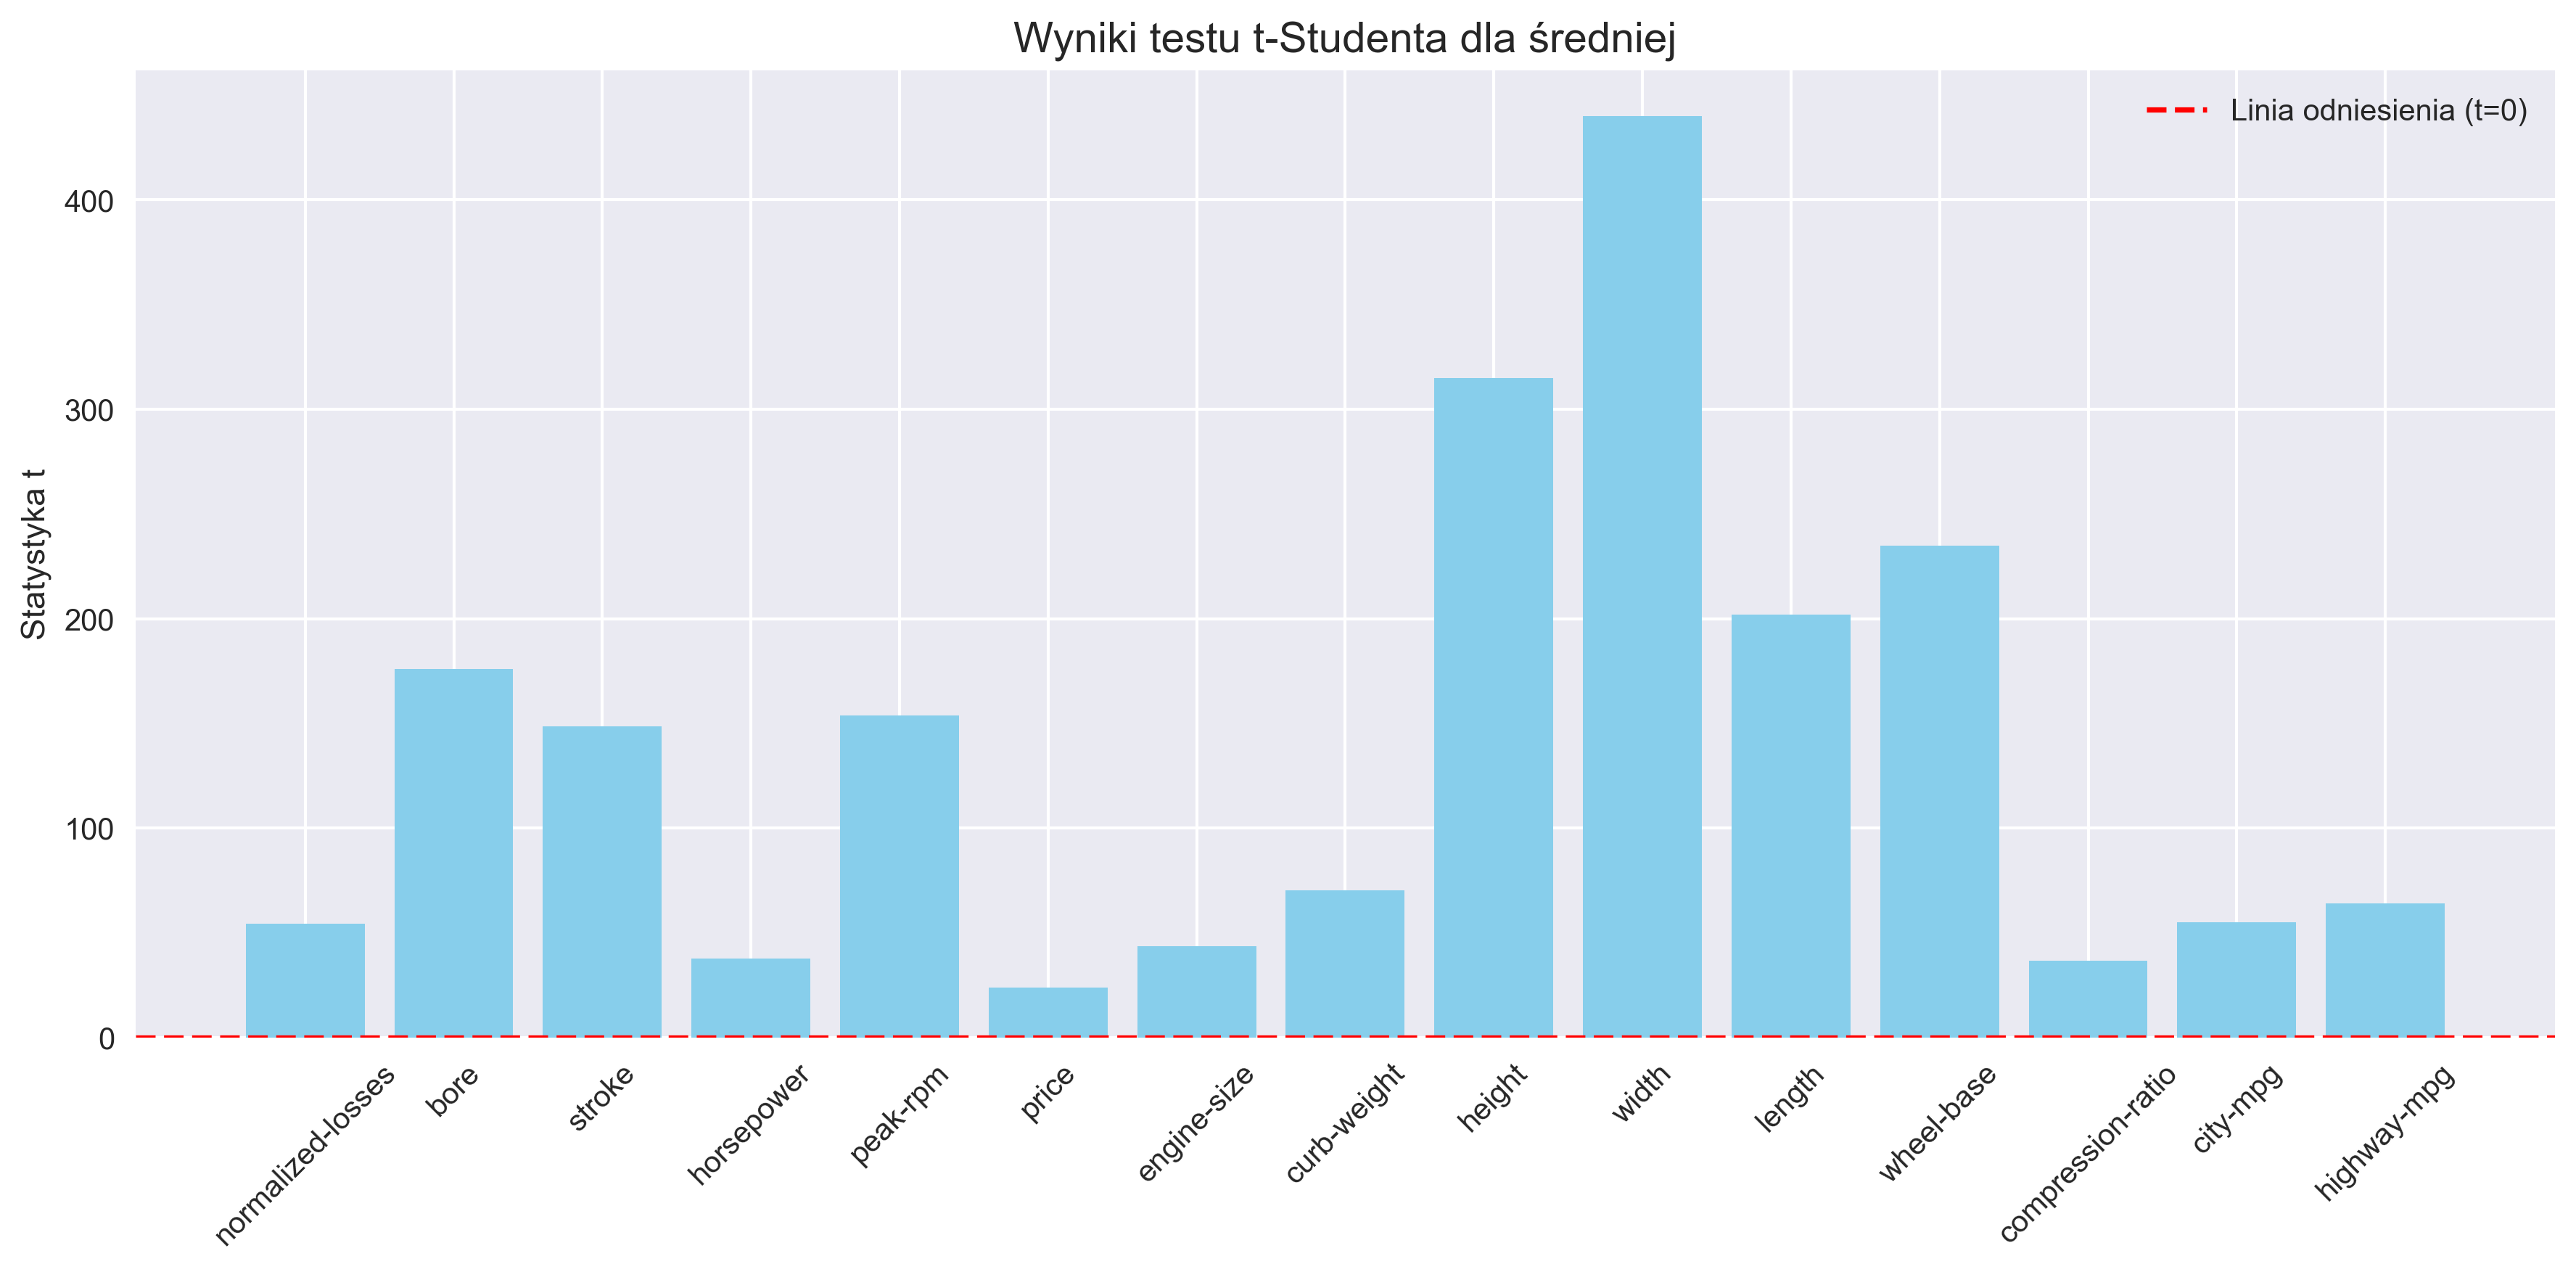
\includegraphics[width=\textwidth]{figures/ttest_statistics.png}
        \caption{Statystyki testu t-Studenta}
    \end{subfigure}
    \hfill
    \begin{subfigure}[b]{0.48\textwidth}
        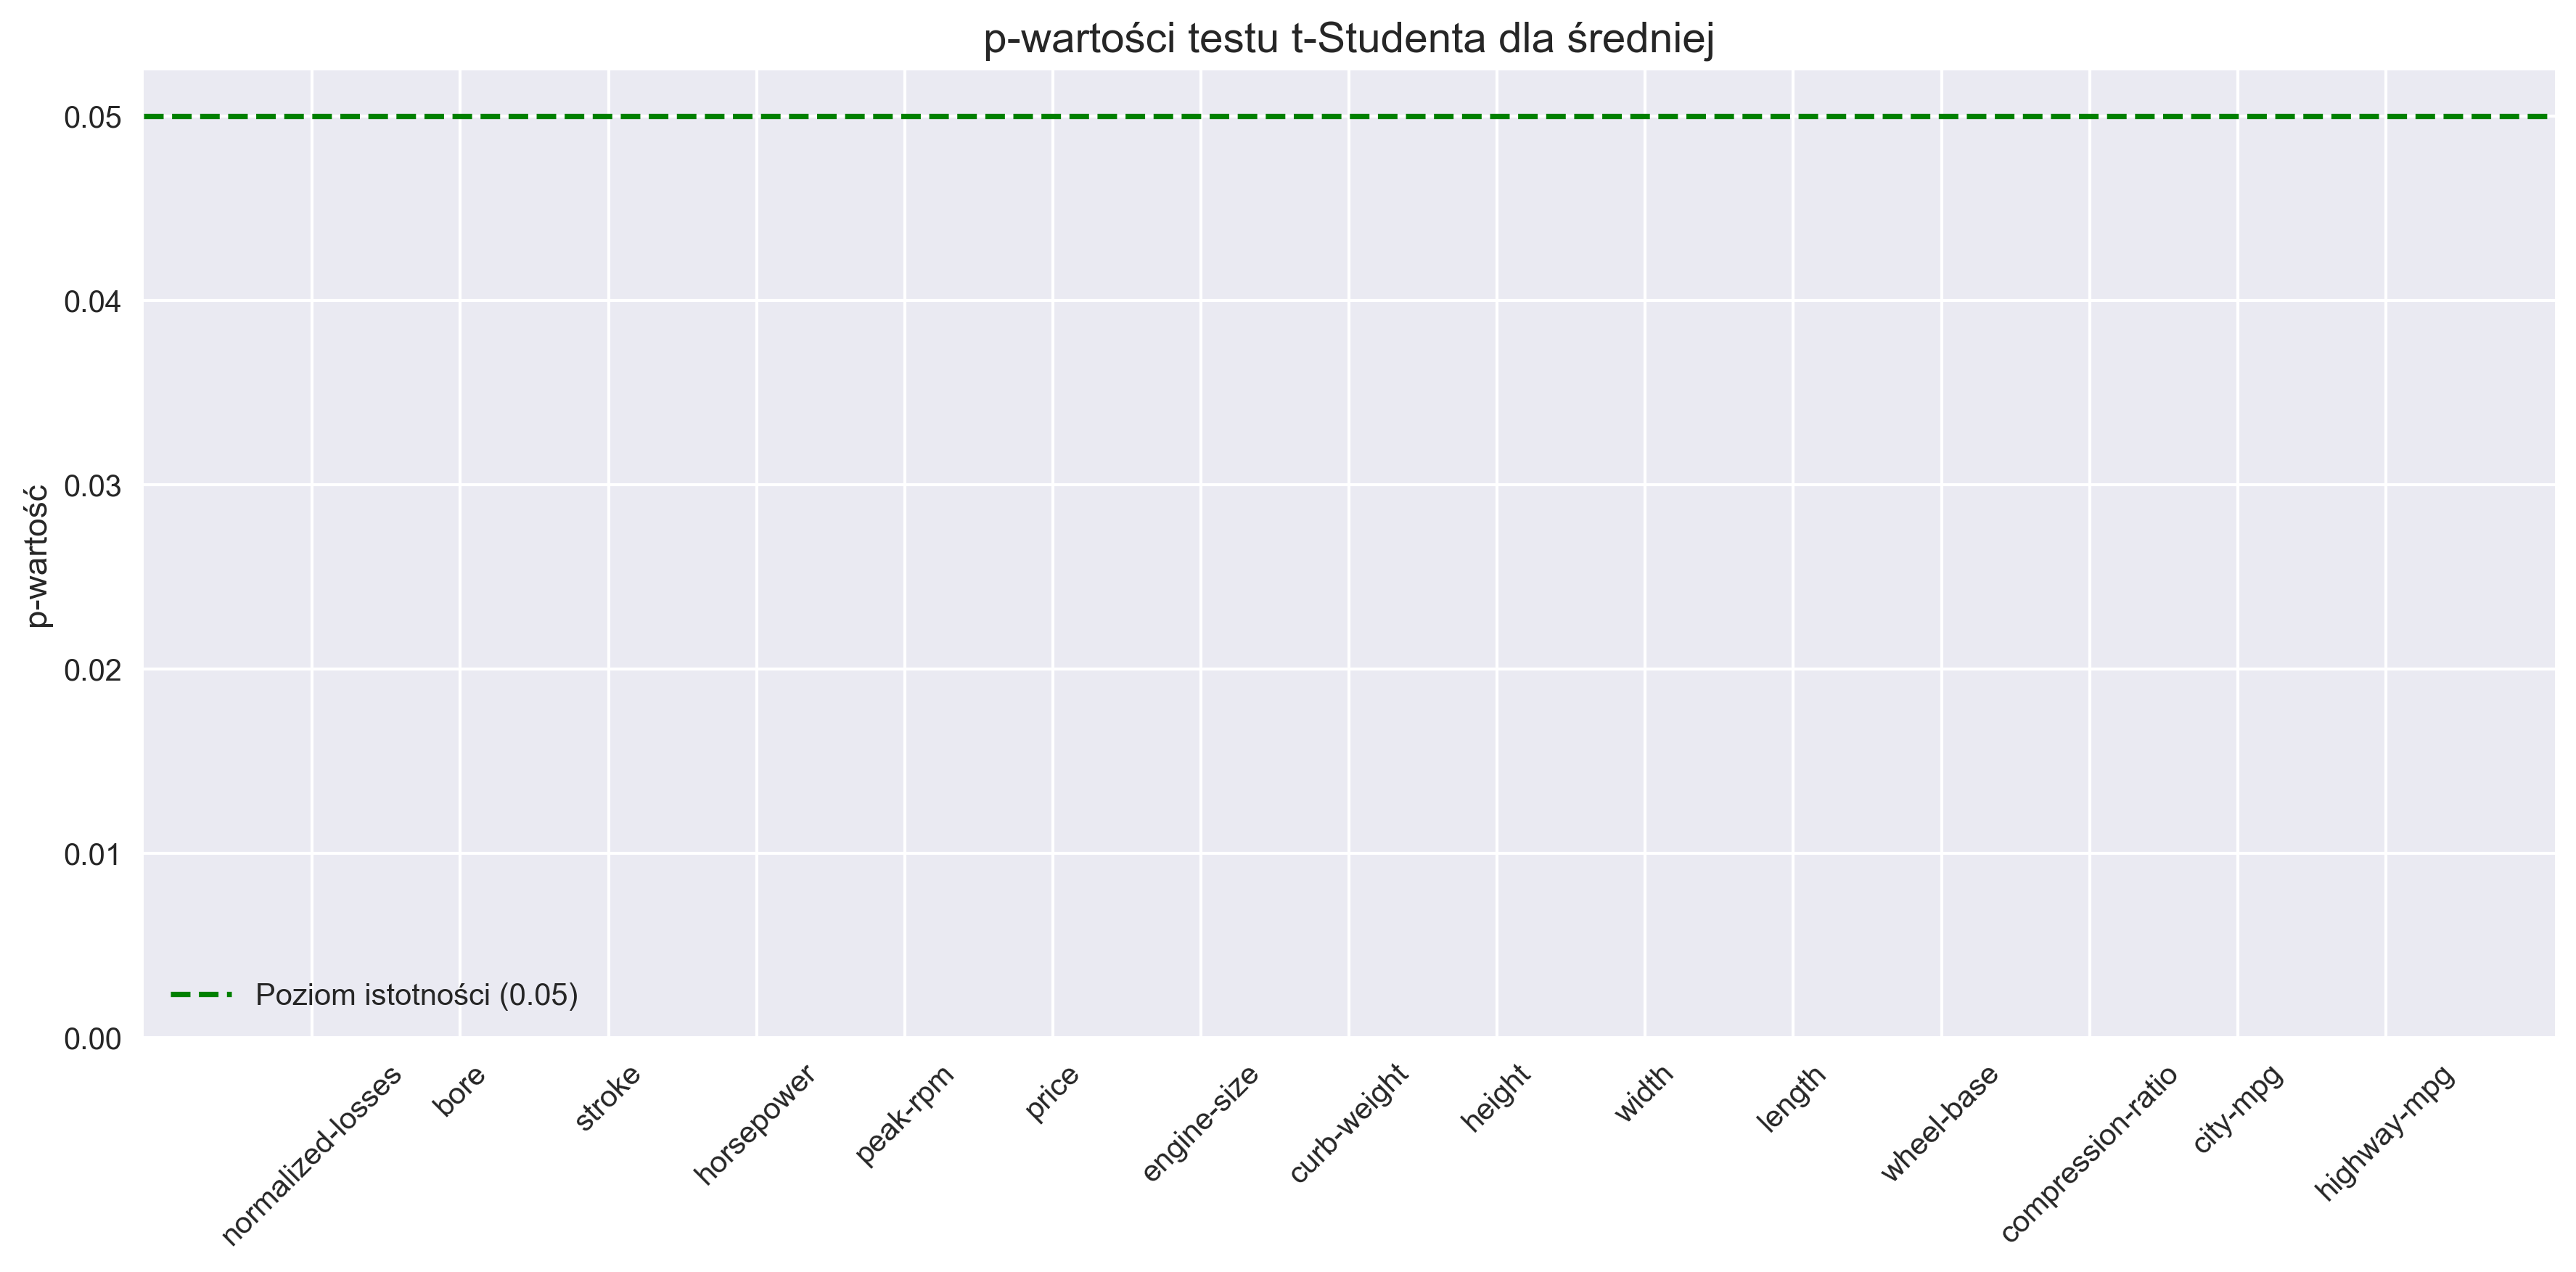
\includegraphics[width=\textwidth]{figures/ttest_pvalues.png}
        \caption{p-wartosci testu t-Studenta}
    \end{subfigure}
    \caption{Wyniki testu t-Studenta dla sredniej}
    \label{fig:ttest_results}
\end{figure}

\subsection{Test t-Studenta dla sredniej}

Wyniki testu t-Studenta zostały przedstawione na Rys.~\ref{fig:ttest_results}.

\textbf{Wnioski:}

\begin{itemize}
    \item Wszystkie zmienne mają \textbf{wartosci p znacznie poniżej progu istotnosci 0.05}, co oznacza, że \textbf{srednia każdej zmiennej jest istotnie różna od zera}.
    \item Szczególnie wysokie statystyki t zaobserwowano dla cech takich jak \texttt{width}, \texttt{height}, \texttt{wheel-base} czy \texttt{length} — oznacza to, że ich srednie są silnie oddalone od zera w ujęciu statystycznym.
    \item Wyniki te potwierdzają, że zmienne te zawierają \textbf{informację statystycznie istotną} i mogą byc brane pod uwagę przy dalszym modelowaniu lub analizach.
\end{itemize}

\begin{figure}[H]
    \centering
    \begin{subfigure}[b]{0.48\textwidth}
        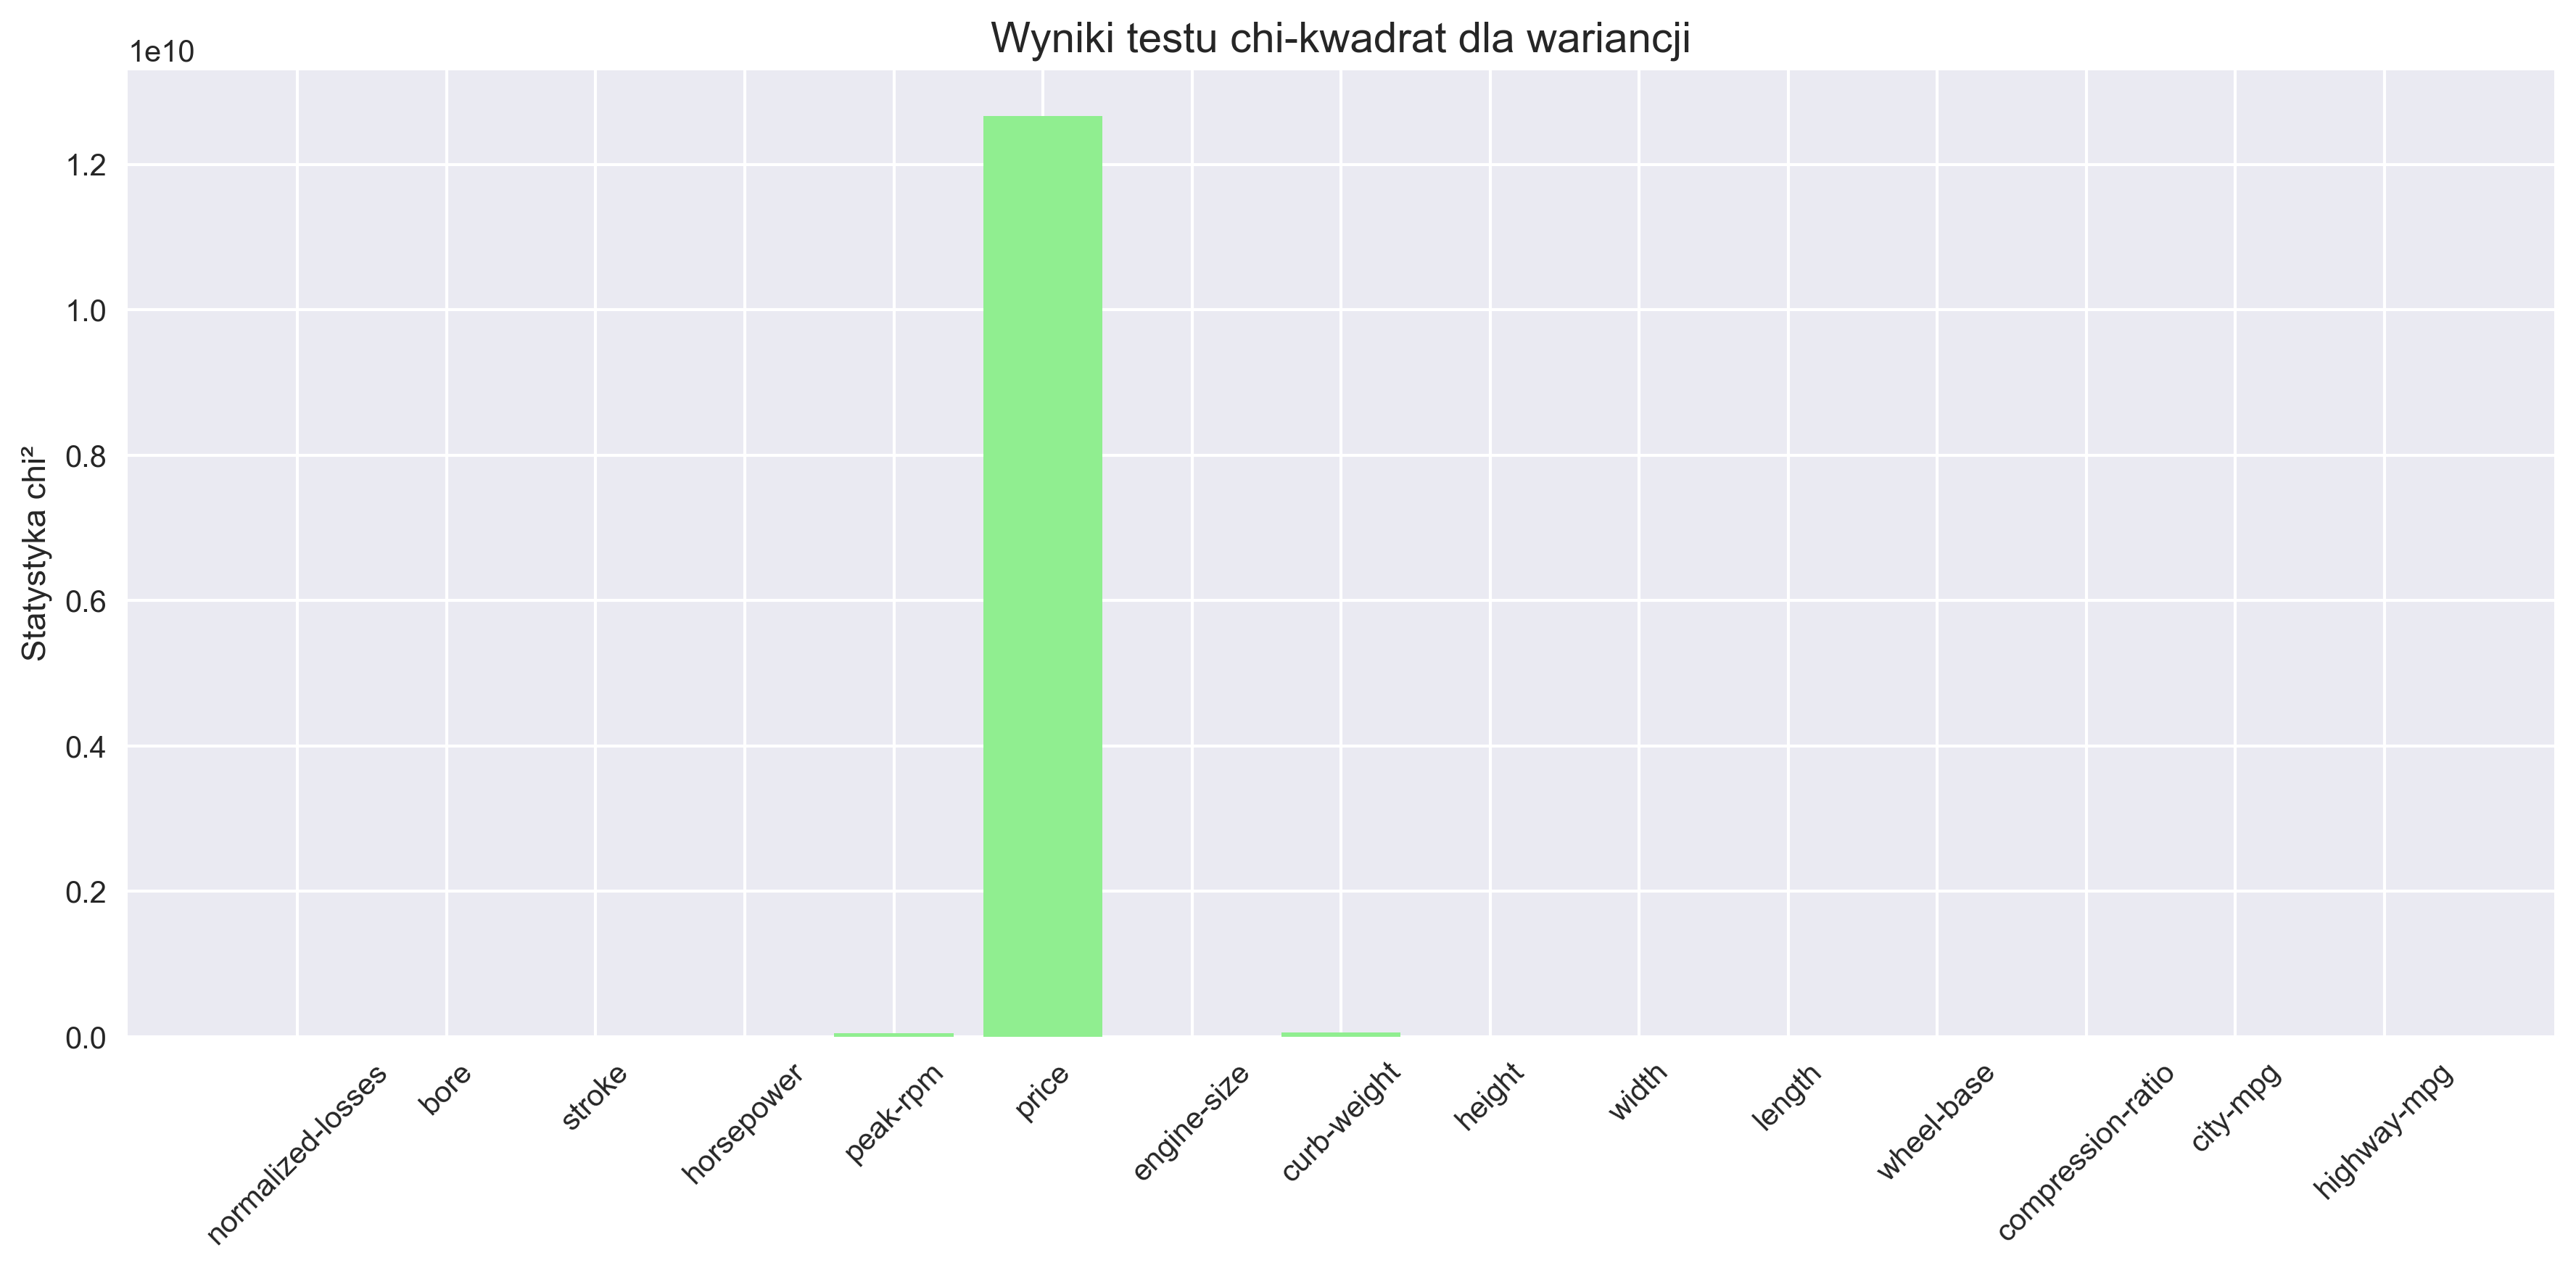
\includegraphics[width=\textwidth]{figures/chi2_statistics.png}
        \caption{Statystyki testu chi-kwadrat}
    \end{subfigure}
    \hfill
    \begin{subfigure}[b]{0.48\textwidth}
        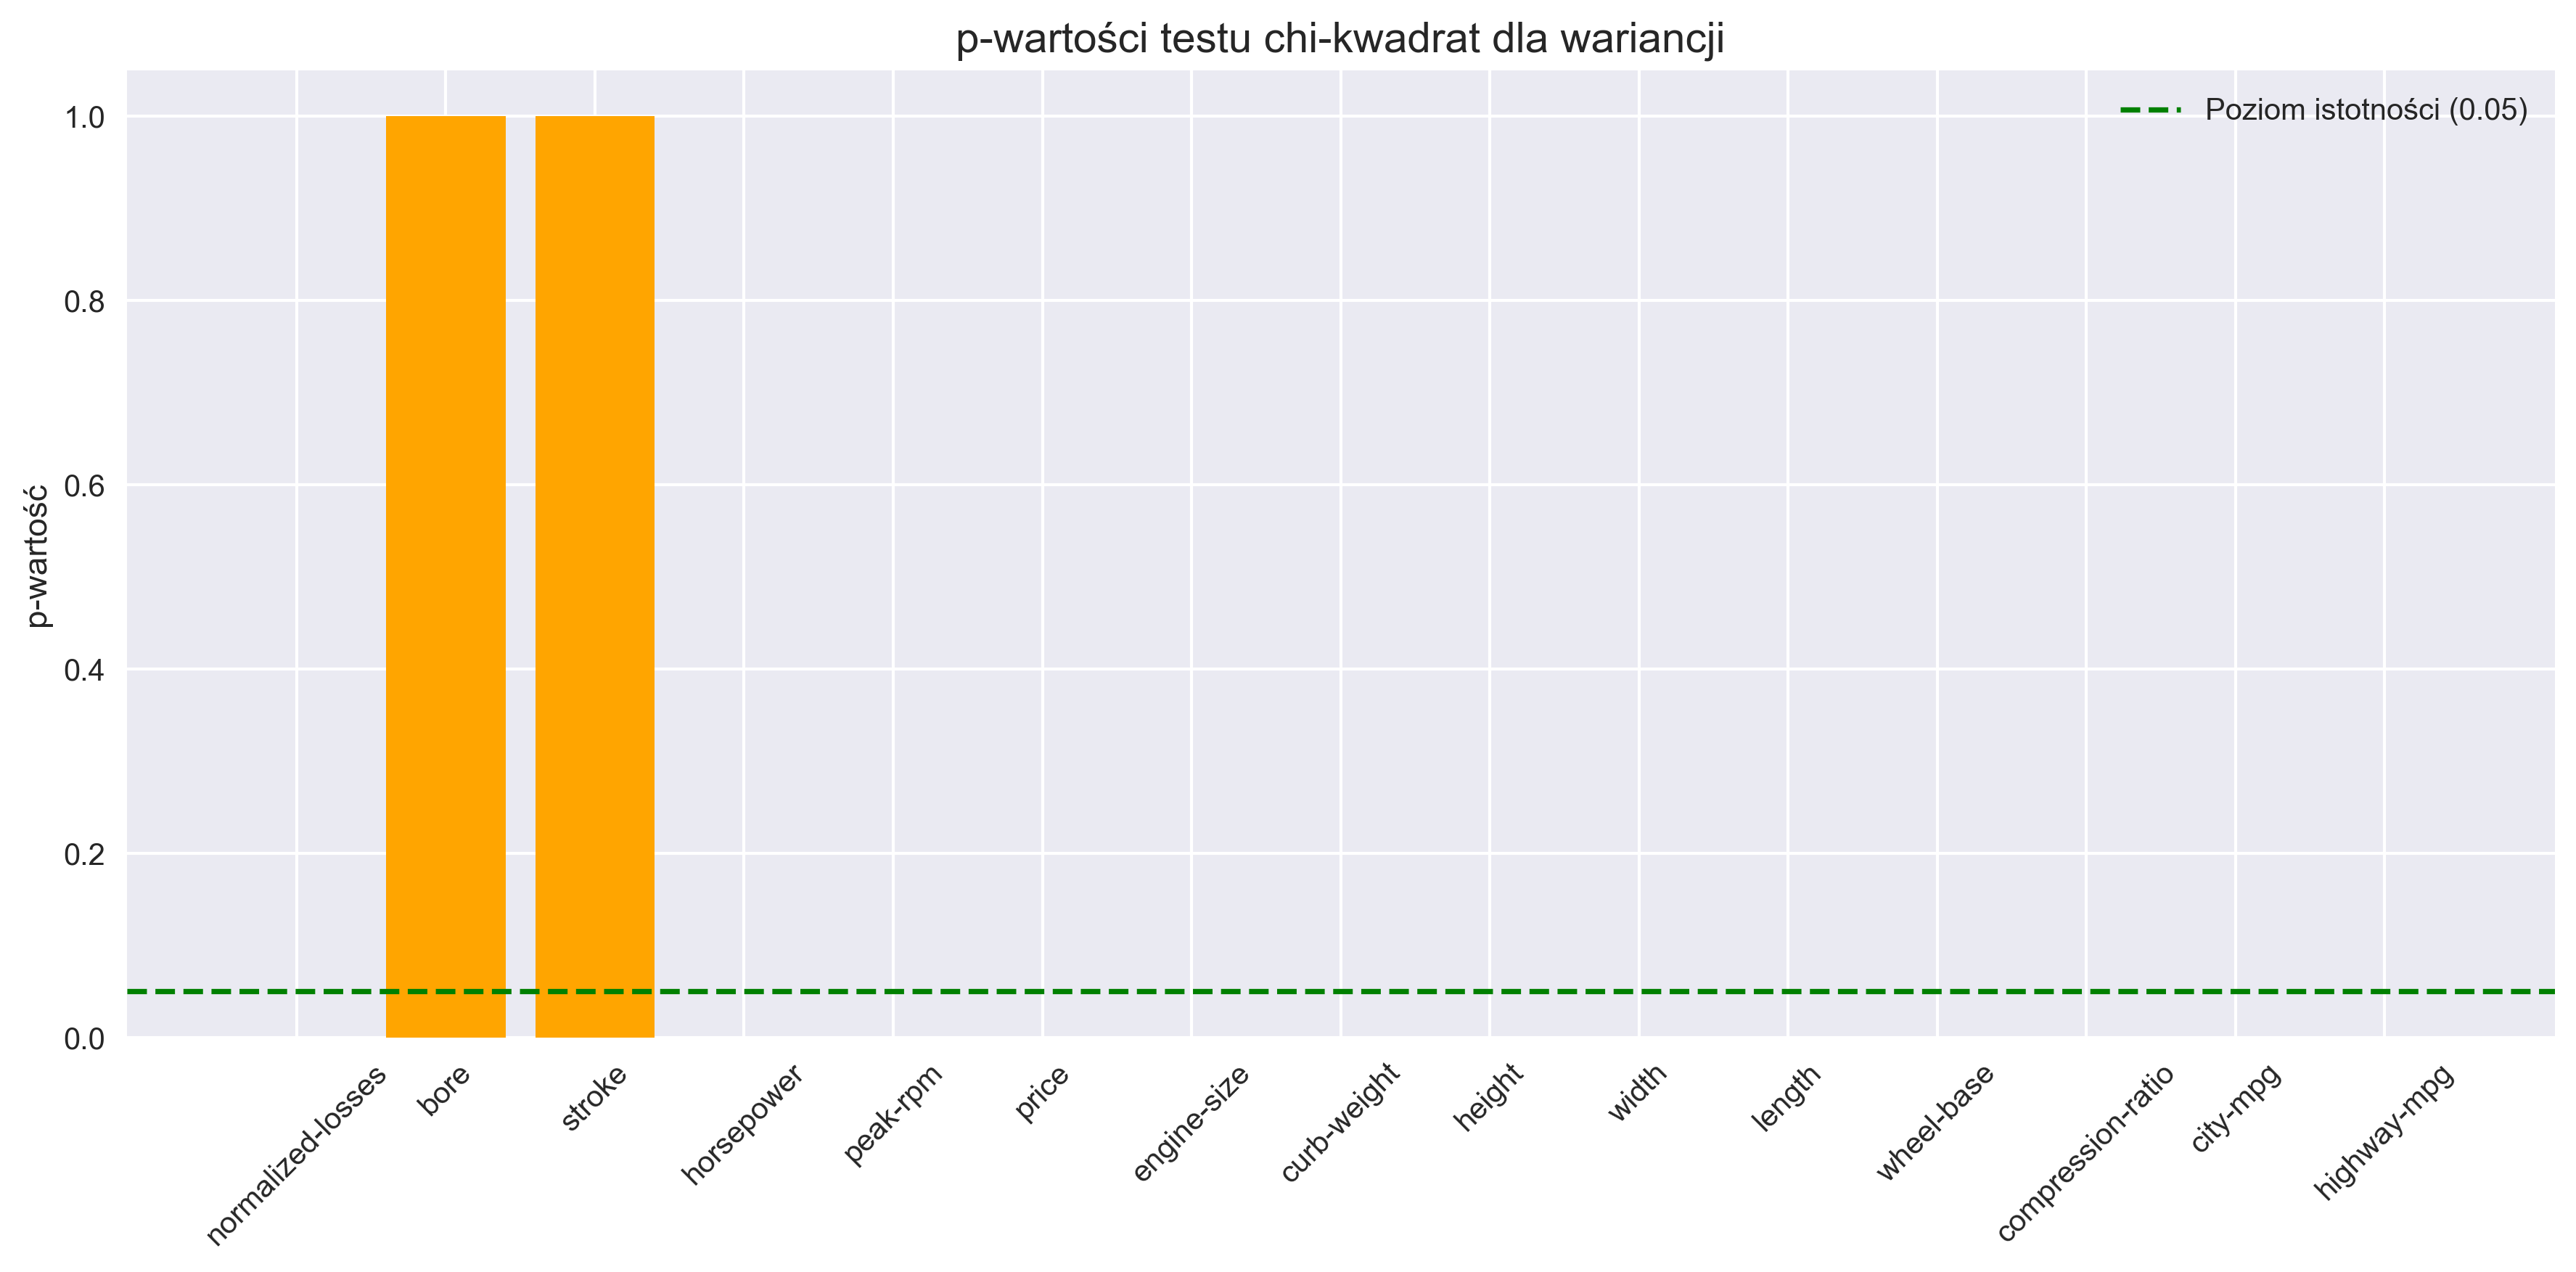
\includegraphics[width=\textwidth]{figures/chi2_pvalues.png}
        \caption{p-wartosci testu chi-kwadrat}
    \end{subfigure}
    \caption{Wyniki testu chi-kwadrat dla wariancji}
    \label{fig:chi2_results}
\end{figure}

\subsection{Test chi-kwadrat dla wariancji}

Wyniki testu chi-kwadrat przedstawiono na Rys.~\ref{fig:chi2_results}.

\textbf{Wnioski:}

\begin{itemize}
    \item Większosc zmiennych wykazuje \textbf{p-wartosci poniżej poziomu istotnosci 0.05}, co oznacza, że ich wariancje \textbf{różnią się istotnie od wartosci oczekiwanej} (hipotezy zerowej).
    \item Wyjątkiem są zmienne \texttt{bore} i \texttt{stroke}, których \textbf{p-wartosci są bliskie 1}, co wskazuje na \textbf{brak podstaw do odrzucenia hipotezy zerowej} – wariancje tych zmiennych są zgodne z teoretycznym założeniem.
    \item Szczególnie wyróżnia się zmienna \texttt{price}, która osiąga \textbf{bardzo wysoką statystykę chi²}, co oznacza \textbf{dużą niestabilnosc wariancji} — warto rozważyc jej przekształcenie (np. transformację logarytmiczną).
\end{itemize}

\subsection{Podsumowanie}

Analiza testów statystycznych pozwala wyciągnąc następujące wnioski:

\begin{itemize}
    \item \textbf{srednie wszystkich zmiennych są istotnie różne od zera}, co wskazuje na ich przydatnosc w dalszych analizach.
    \item \textbf{Większosc zmiennych ma istotnie różną wariancję}, co może sugerowac koniecznosc standaryzacji lub transformacji niektórych cech (szczególnie \texttt{price}).
    \item Zmiennych \texttt{bore} i \texttt{stroke} \textbf{nie trzeba transformowac pod względem wariancji}, gdyż nie wykazują odchyleń względem założeń testu.
\end{itemize}

Wyniki te wspierają decyzje dotyczące dalszego przygotowania danych, m.in. selekcji cech, normalizacji lub inżynierii cech.

\subsection{Kod implementujący testy statystyczne}
\begin{lstlisting}[language=Python, caption=Kod testów dla sredniej i wariancji]
import os
import numpy as np
import matplotlib.pyplot as plt
from scipy import stats

# Ensure figures directory exists
if not os.path.exists('figures'):
    os.makedirs('figures')

t_stats = []
p_values_t = []

for var in continuous_vars:
    data = df[var].dropna()
    t_stat, p_value = stats.ttest_1samp(data, 0)
    t_stats.append(t_stat)
    p_values_t.append(p_value)

# Plot for t-statistics
plt.figure(figsize=(12, 6))
plt.bar(continuous_vars, t_stats, color='skyblue')
plt.axhline(y=0, color='red', linestyle='--', label='Linia odniesienia (t=0)')
plt.title('Wyniki testu t-Studenta dla sredniej', fontsize=14)
plt.ylabel('Statystyka t')
plt.xticks(rotation=45)
plt.legend()
plt.tight_layout()
plt.savefig('figures/ttest_statistics.png', dpi=300, bbox_inches='tight')
plt.show()

# Plot for t-test p-values
plt.figure(figsize=(12, 6))
plt.bar(continuous_vars, p_values_t, color='salmon')
plt.axhline(y=0.05, color='green', linestyle='--', label='Poziom istotnosci (0.05)')
plt.title('p-wartosci testu t-Studenta dla sredniej', fontsize=14)
plt.ylabel('p-wartosc')
plt.xticks(rotation=45)
plt.legend()
plt.tight_layout()
plt.savefig('figures/ttest_pvalues.png', dpi=300, bbox_inches='tight')
plt.show()

chi2_stats = []
p_values_chi2 = []

for var in continuous_vars:
    data = df[var].dropna()
    n = len(data)
    sample_var = np.var(data, ddof=1)
    chi2_stat = (n - 1) * sample_var / 1
    p_value = stats.chi2.sf(chi2_stat, df=n-1)
    chi2_stats.append(chi2_stat)
    p_values_chi2.append(p_value)

# Plot for chi-squared statistics
plt.figure(figsize=(12, 6))
plt.bar(continuous_vars, chi2_stats, color='lightgreen')
plt.title('Wyniki testu chi-kwadrat dla wariancji', fontsize=14)
plt.ylabel('Statystyka chi²')
plt.xticks(rotation=45)
plt.tight_layout()
plt.savefig('figures/chi2_statistics.png', dpi=300, bbox_inches='tight')
plt.show()

# Plot for chi-squared p-values
plt.figure(figsize=(12, 6))
plt.bar(continuous_vars, p_values_chi2, color='orange')
plt.axhline(y=0.05, color='green', linestyle='--', label='Poziom istotnosci (0.05)')
plt.title('p-wartosci testu chi-kwadrat dla wariancji', fontsize=14)
plt.ylabel('p-wartosc')
plt.xticks(rotation=45)
plt.legend()
plt.tight_layout()
plt.savefig('figures/chi2_pvalues.png', dpi=300, bbox_inches='tight')
plt.show()
\end{lstlisting}

\section{Estymator jądrowy gęstosci}

W celu analizy rozkładu zmiennych numerycznych w zbiorze danych Automobile przeprowadzono estymację jądrową gęstosci (KDE) dla każdej z cech. Metoda ta umożliwia wygładzenie histogramów i lepsze zrozumienie kształtu rozkładu danych bez wpływu liczby przedziałów histogramu.

\begin{figure}[H]
    \centering
    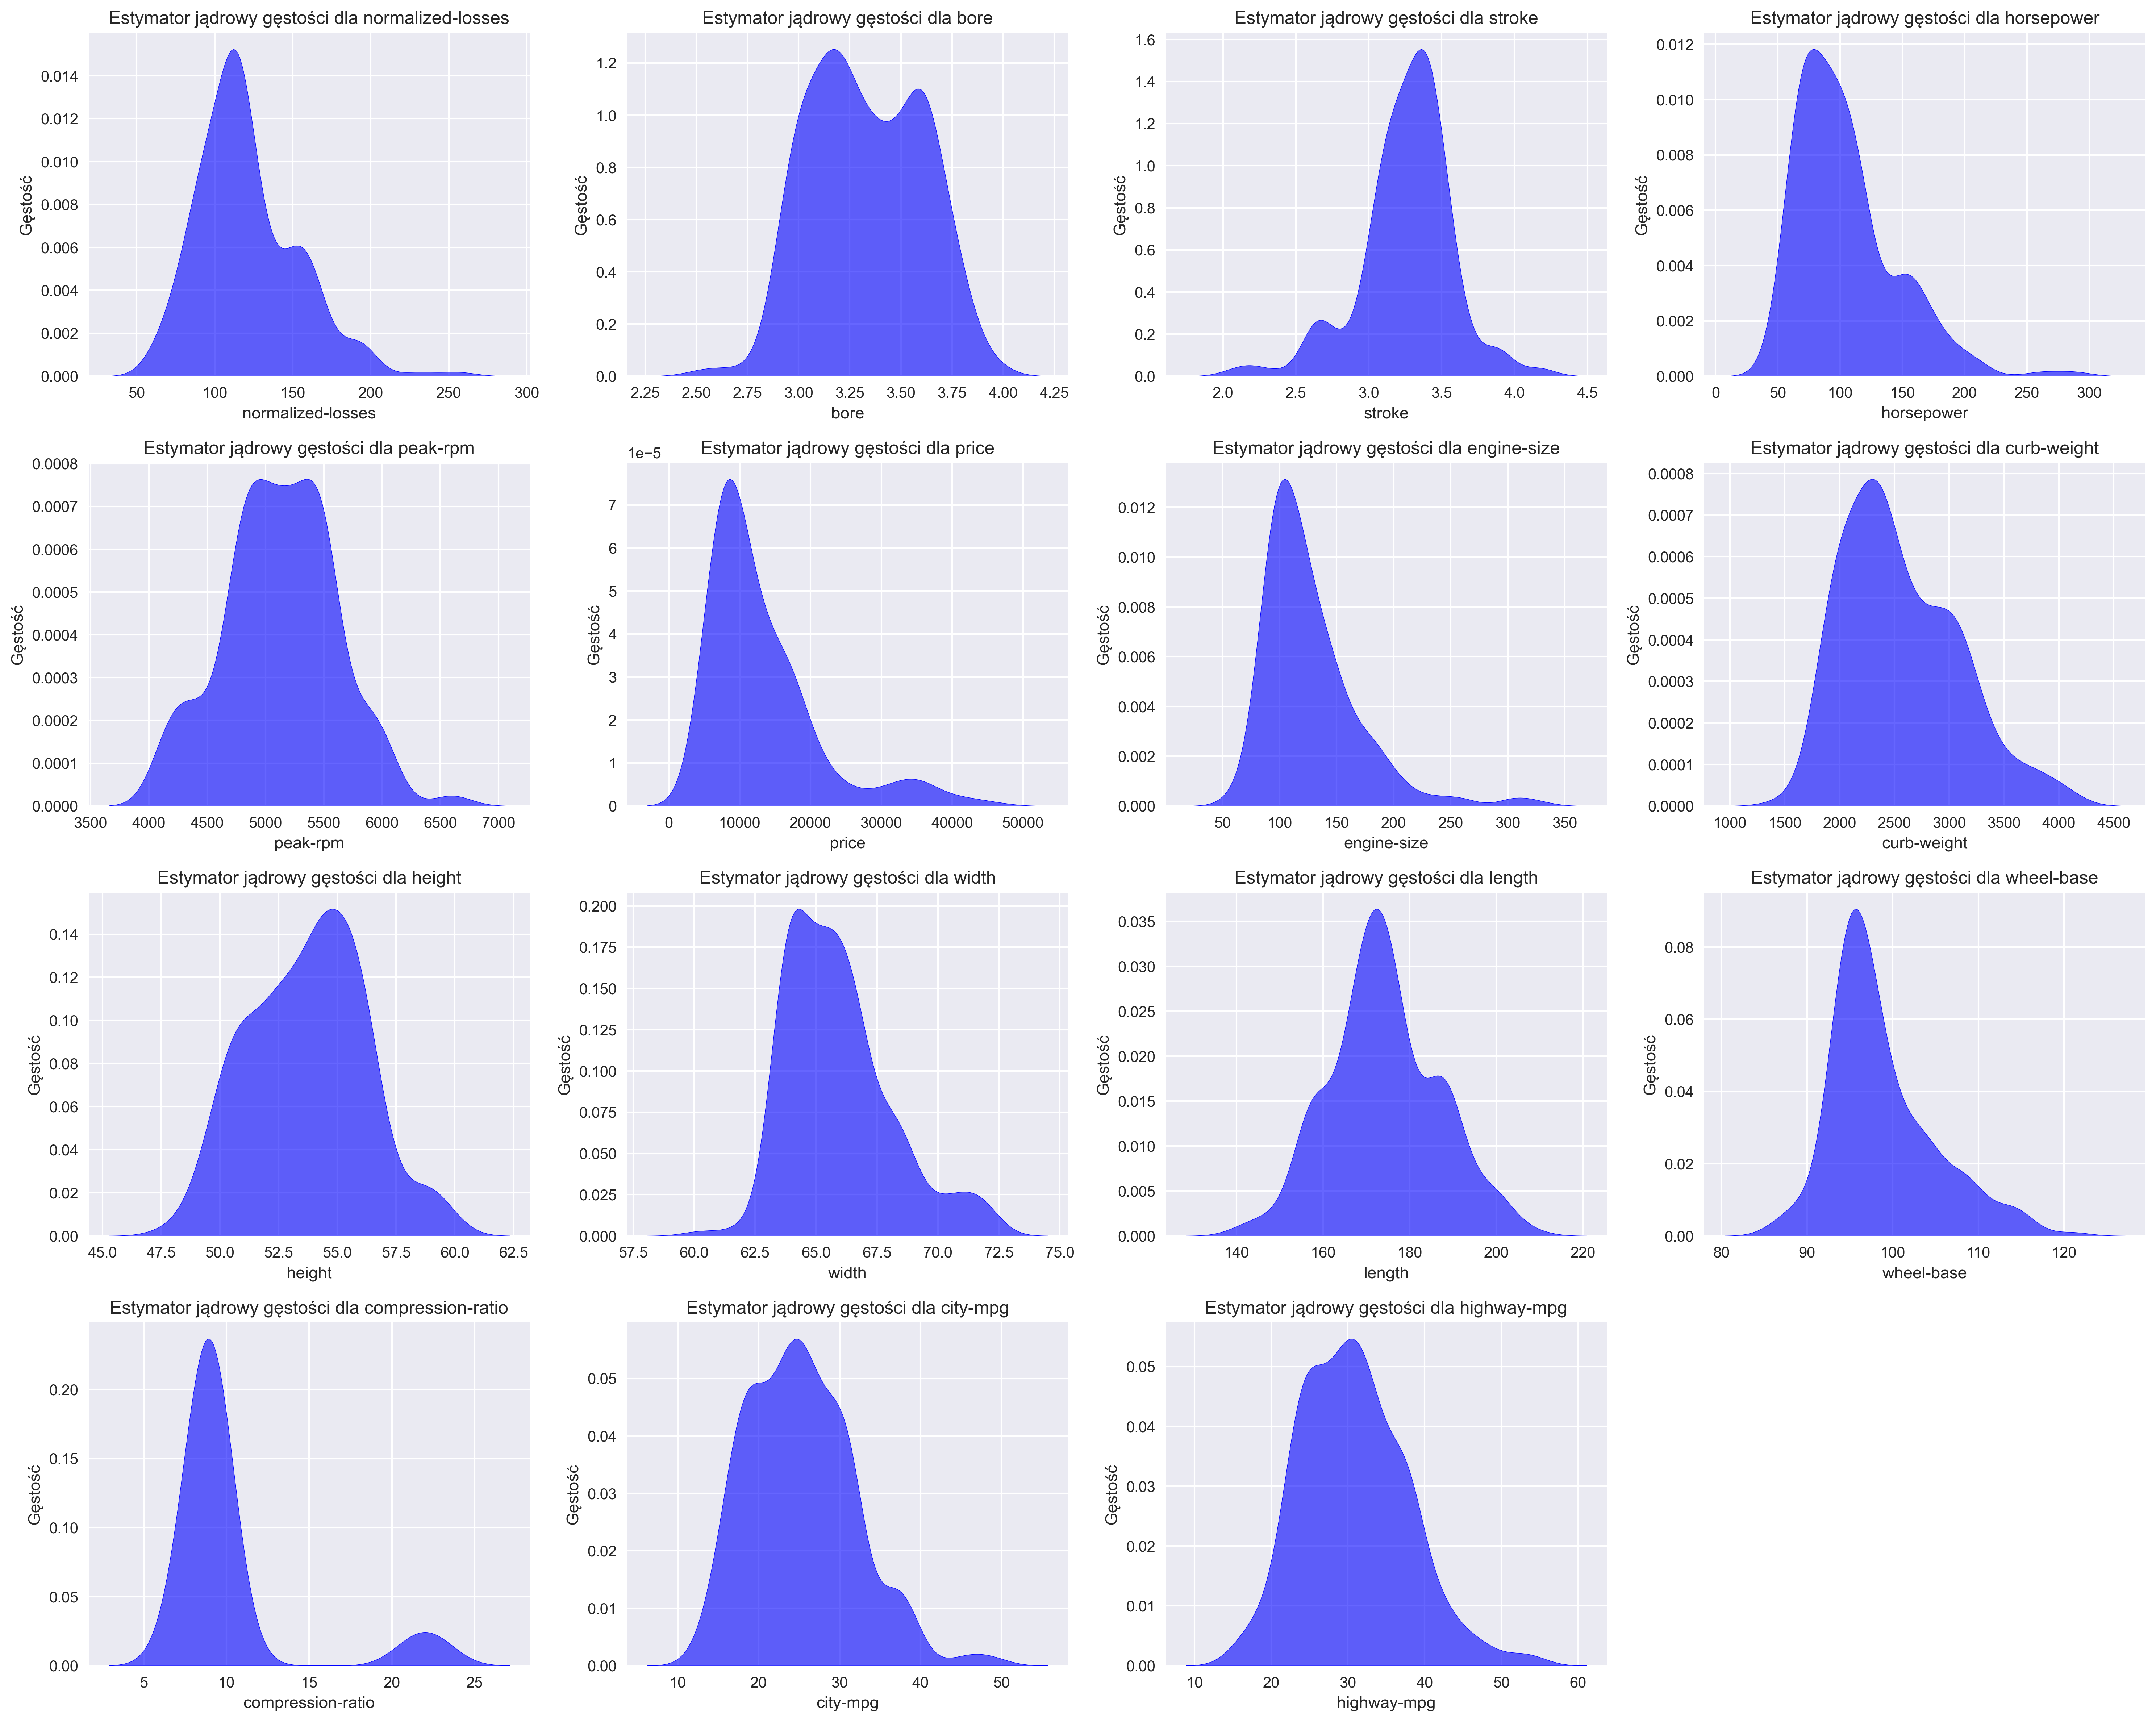
\includegraphics[width=0.9\textwidth]{figures/kde_plots_all_variables.png}
    \caption{Estymatory jądrowe gęstosci dla wszystkich zmiennych ciągłych}
    \label{fig:kde_plots_all_variables}
\end{figure}

\subsection{Wnioski z wykresów KDE}

\begin{itemize}
    \item \textbf{Wiele zmiennych ma rozkład asymetryczny} – m.in. \texttt{price}, \texttt{horsepower}, \texttt{engine-size} oraz \texttt{compression-ratio} cechują się długim ogonem po prawej stronie. Sugeruje to obecnosc wartosci odstających (ang. \textit{outliers}) – pojedynczych, nietypowo wysokich wartosci.

    \item \textbf{Niektóre zmienne mają rozkład zbliżony do normalnego} – np. \texttt{peak-rpm}, \texttt{height} i \texttt{width} są skupione wokół jednej dominującej wartosci, co może odzwierciedlac standardy konstrukcyjne wsród producentów samochodów.

    \item \textbf{Zmienna \texttt{compression-ratio} wykazuje rozkład dwumodalny}, co może sugerowac obecnosc dwóch różnych klas silników (np. benzynowe vs. wysokoprężne).

    \item \textbf{Zmienne \texttt{normalized-losses} i \texttt{price} cechuje duża rozpiętosc wartosci}, co może wymagac dalszego przekształcenia danych (np. transformacji logarytmicznej, standaryzacji) w celu poprawy jakosci modeli predykcyjnych.

    \item \textbf{Rozkłady \texttt{city-mpg} oraz \texttt{highway-mpg} są przesunięte ku lewej}, co oznacza, że większosc samochodów ma umiarkowane zużycie paliwa, a jedynie nieliczne cechują się bardzo wysoką efektywnoscią.
\end{itemize}

\begin{figure}[H]
    \centering
    \begin{subfigure}[b]{0.48\textwidth}
        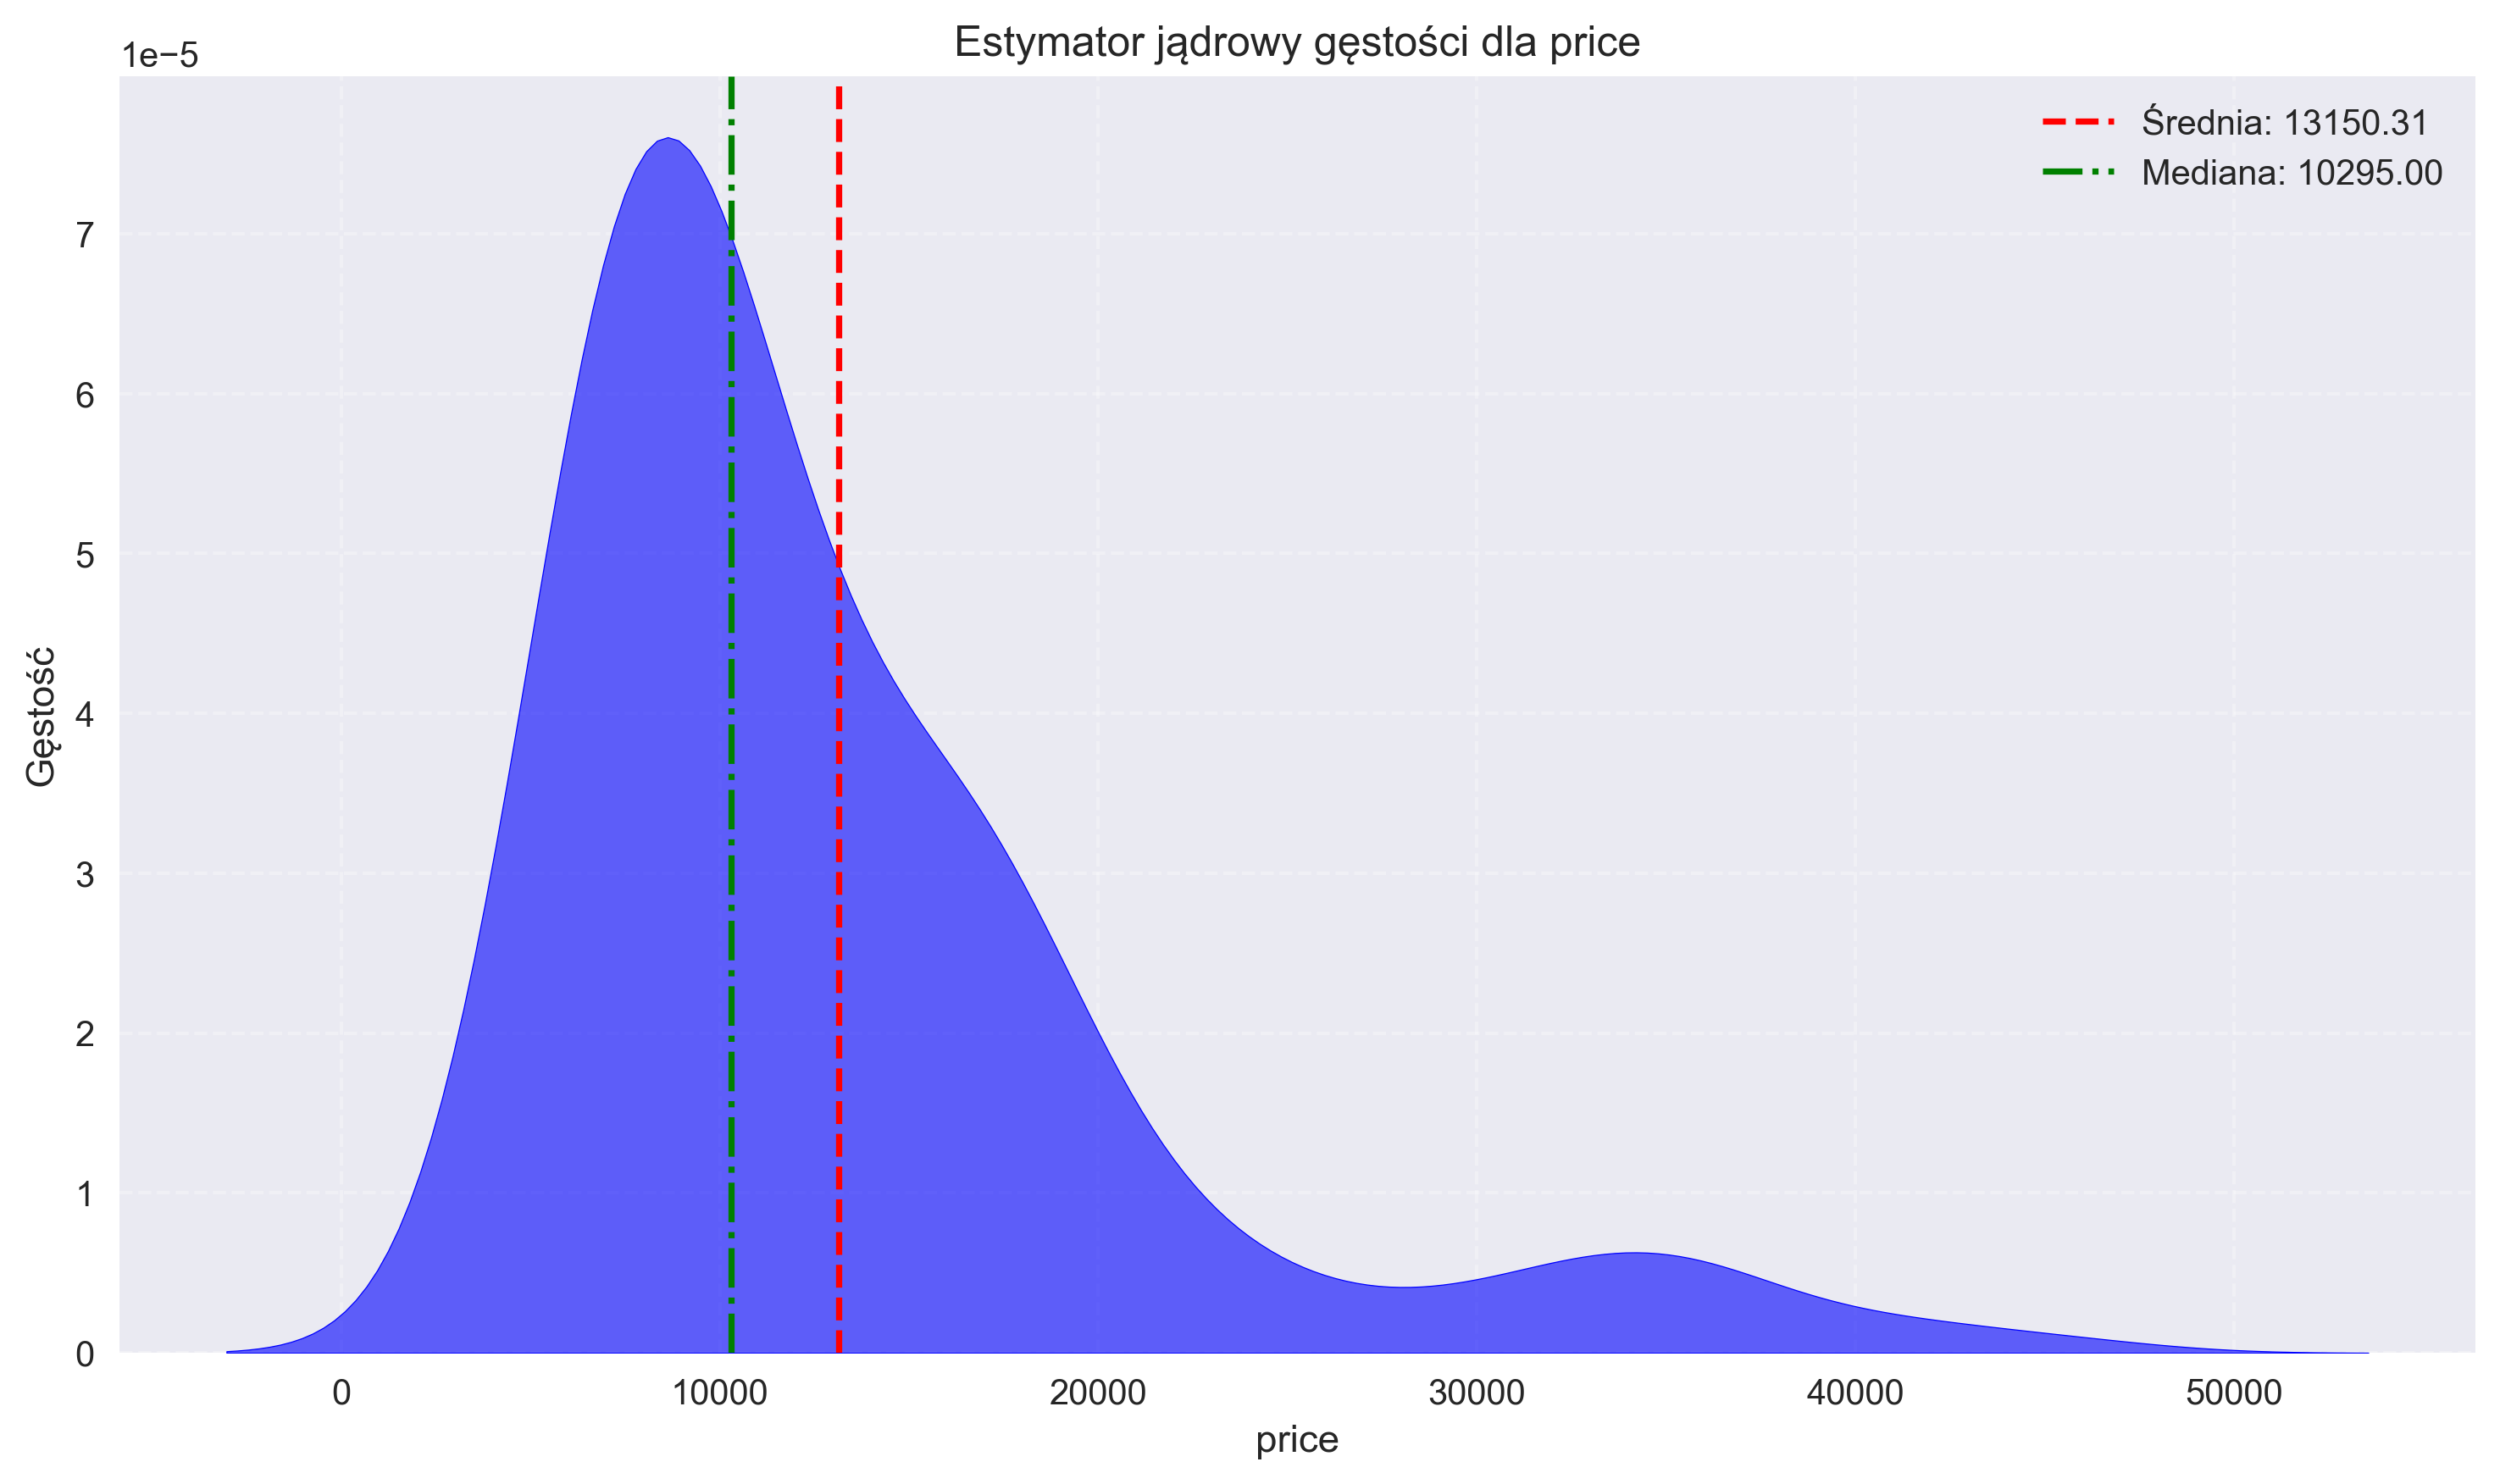
\includegraphics[width=\textwidth]{figures/kde_price.png}
        \caption{Estymator jądrowy gęstosci dla zmiennej price}
    \end{subfigure}
    \hfill
    \begin{subfigure}[b]{0.48\textwidth}
        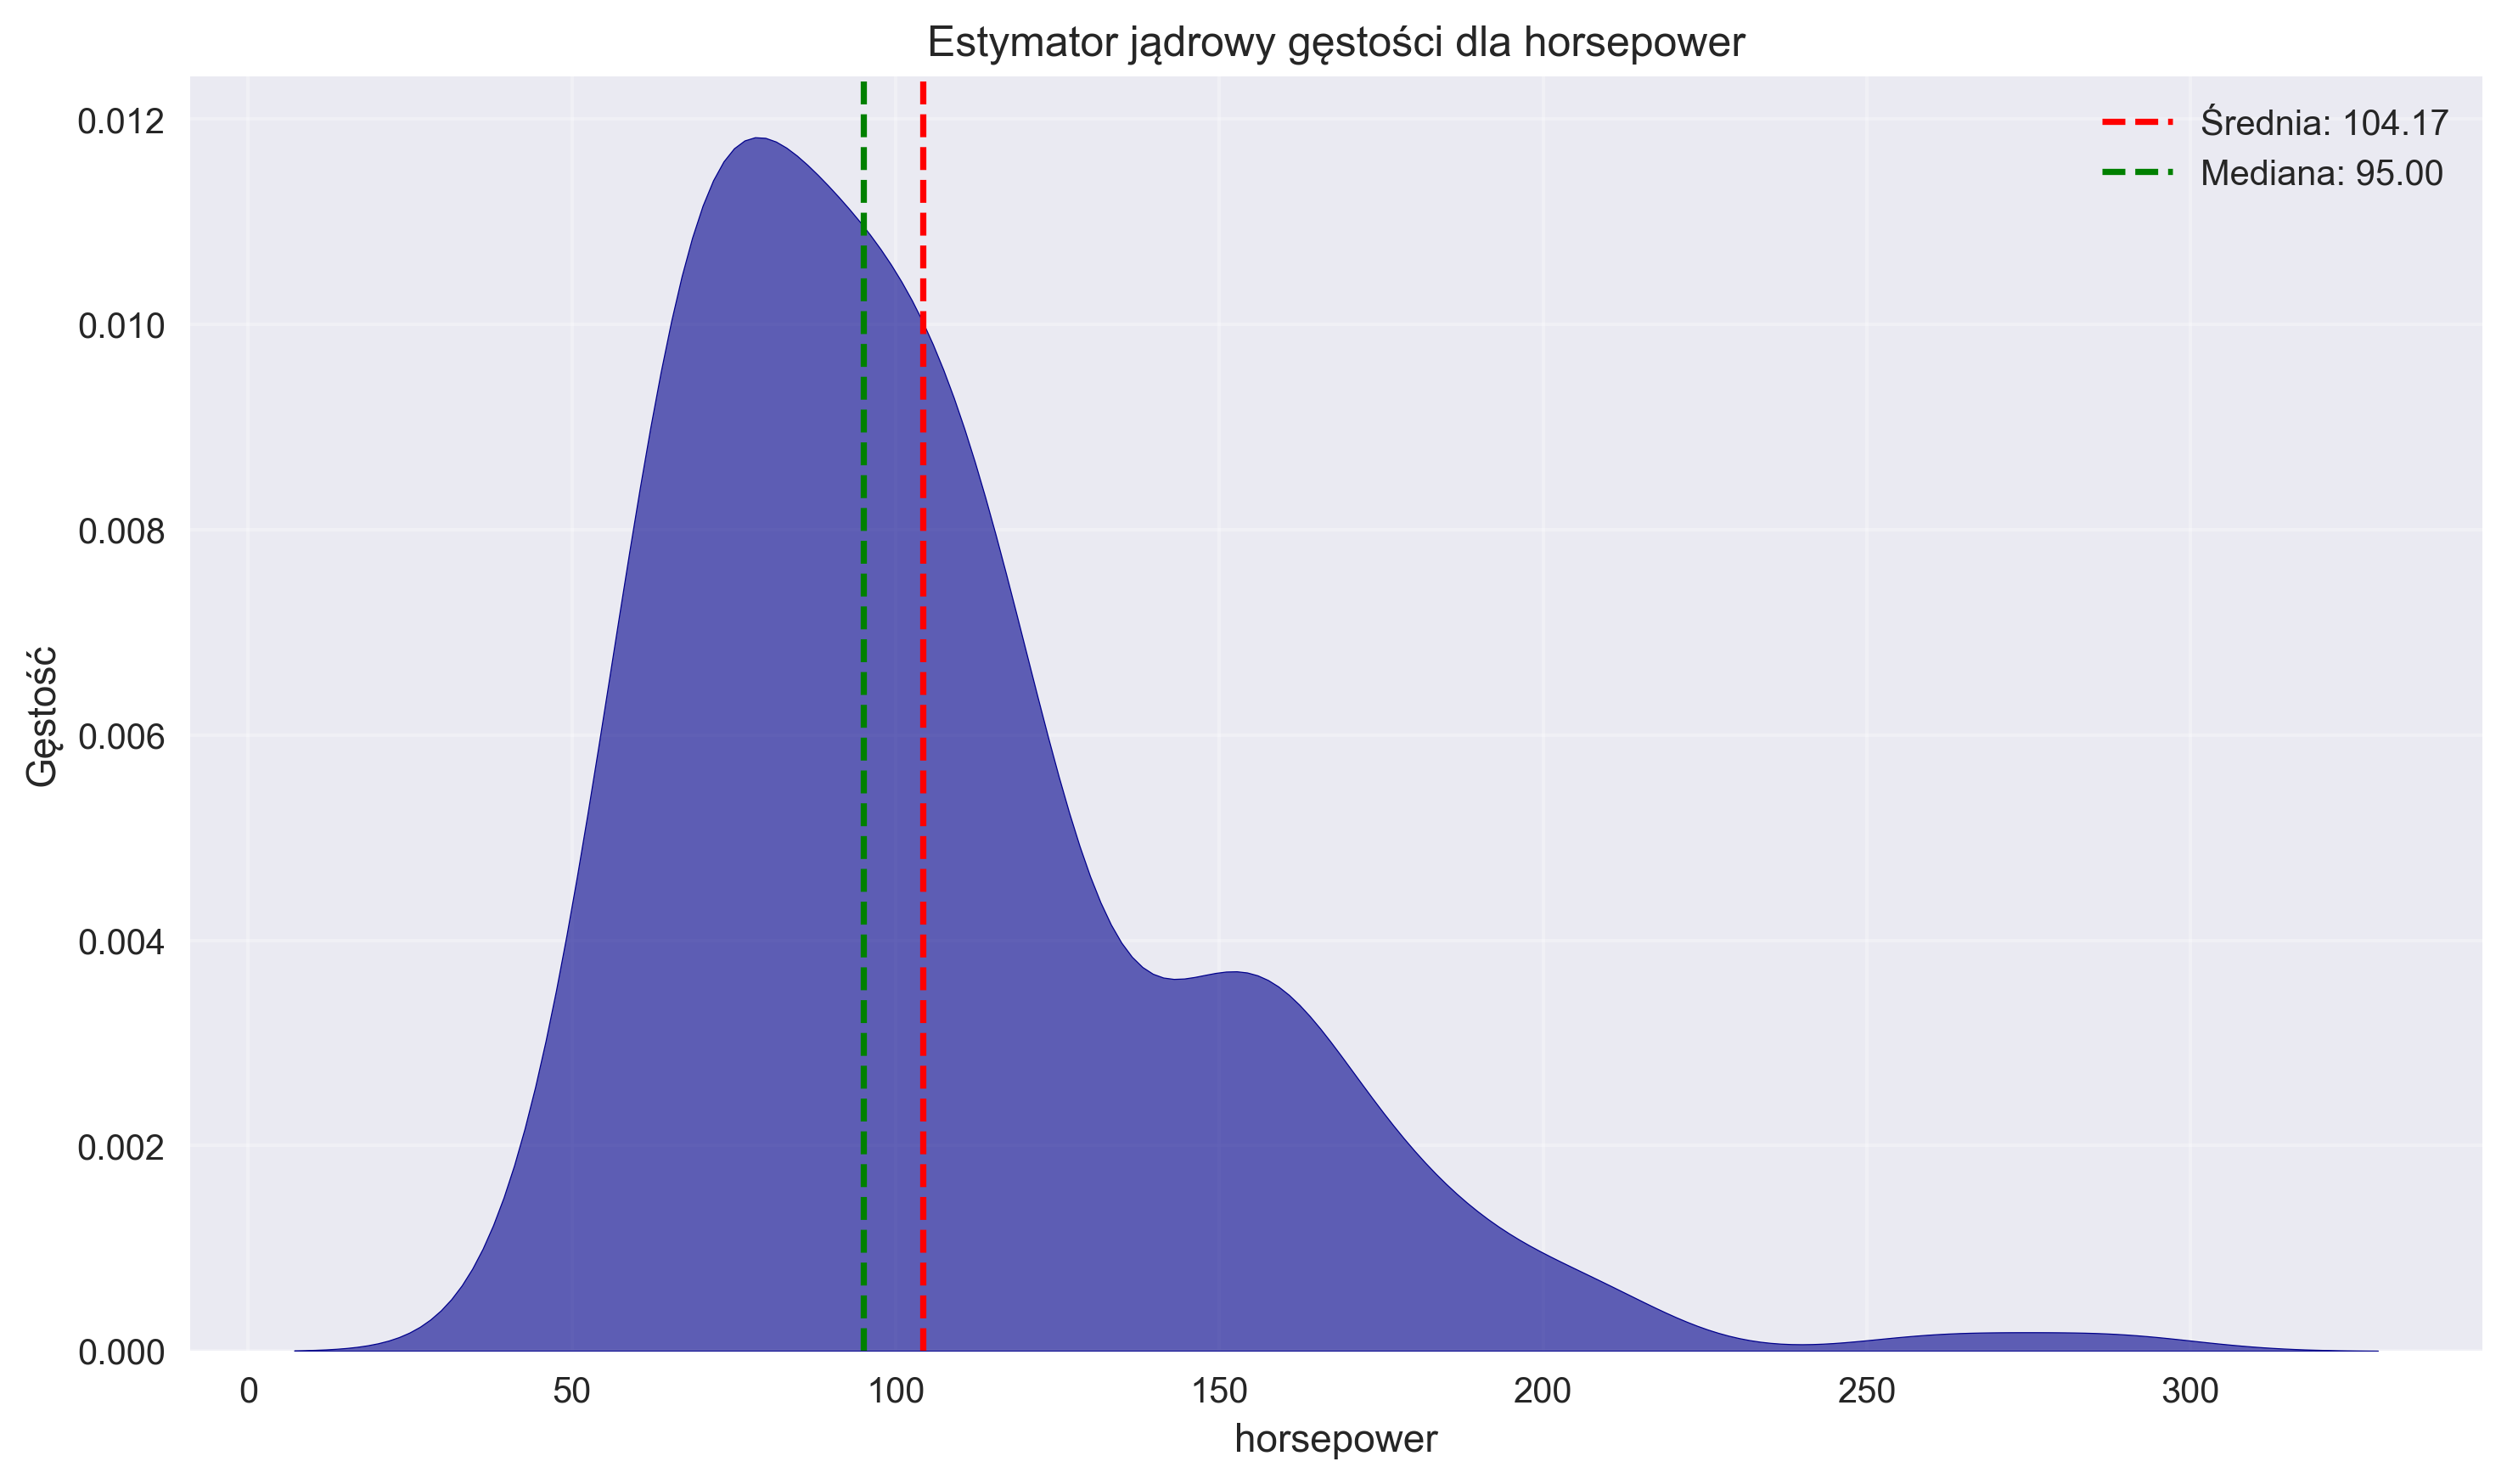
\includegraphics[width=\textwidth]{figures/kde_horsepower.png}
        \caption{Estymator jądrowy gęstosci dla zmiennej horsepower}
    \end{subfigure}
    \caption{Szczegółowe estymatory jądrowe gęstosci dla wybranych zmiennych}
    \label{fig:kde_selected}
\end{figure}

\subsection{Znaczenie analizy KDE}

Estymatory jądrowe gęstosci pozwalają lepiej zrozumiec strukturę danych, wykryc potencjalne problemy (takie jak wartosci odstające, wielomodalnosc rozkładu czy zmiennosc) oraz dobrac odpowiednie transformacje zmiennych. Analiza ta jest istotna jako etap przygotowawczy przed zastosowaniem algorytmów uczenia maszynowego lub budową modeli statystycznych.

\subsection{Kod implementujący estymatory jądrowe gęstosci}
\begin{lstlisting}[language=Python, caption=Kod generujący estymatory jądrowe gęstosci]
import numpy as np
import pandas as pd
import matplotlib.pyplot as plt
import seaborn as sns
from ucimlrepo import fetch_ucirepo
import os

# Ensure figures directory exists
if not os.path.exists('figures'):
    os.makedirs('figures')

automobile = fetch_ucirepo(id=10)
X = automobile.data.features
y = automobile.data.targets
df = pd.concat([X, y], axis=1)

# Przetworzenie brakujących wartosci w zmiennych ciągłych
for column in continuous_vars:
    df[column] = pd.to_numeric(df[column], errors='coerce')
    df[column] = df[column].fillna(df[column].median())

# Create KDE plots for all continuous variables
fig, axes = plt.subplots(4, 4, figsize=(20, 16))
axes = axes.flatten()

for i, var in enumerate(continuous_vars):
    if i < len(axes):
        sns.kdeplot(df[var], ax=axes[i], fill=True, color='blue', alpha=0.6)
        axes[i].set_title(f'Estymator jądrowy gęstosci dla {var}')
        axes[i].set_xlabel(var)
        axes[i].set_ylabel('Gęstosc')

# Turn off any remaining empty axes
for j in range(len(continuous_vars), len(axes)):
    axes[j].axis('off')

plt.tight_layout()
plt.savefig('figures/kde_plots_all_variables.png', dpi=300, bbox_inches='tight')
plt.show()

# Optional: Create individual KDE plots for each variable 
for var in continuous_vars:
    plt.figure(figsize=(10, 6))
    sns.kdeplot(df[var], fill=True, color='blue', alpha=0.6)
    plt.title(f'Estymator jądrowy gęstosci dla {var}')
    plt.xlabel(var)
    plt.ylabel('Gęstosc')
    plt.grid(alpha=0.3, linestyle='--')
    
    # Add mean and median lines
    plt.axvline(df[var].mean(), color='red', linestyle='--', 
                label=f'srednia: {df[var].mean():.2f}')
    plt.axvline(df[var].median(), color='green', linestyle='-.',
                label=f'Mediana: {df[var].median():.2f}')
    plt.legend()
    
    plt.tight_layout()
    plt.savefig(f'figures/kde_{var.replace("-", "_")}.png', dpi=300, bbox_inches='tight')
    plt.close()
\end{lstlisting}

\section{Podsumowanie}

Przeprowadzona analiza statystyczna zbioru danych Automobile dostarcza kompleksowego obrazu charakterystyk samochodów z roku 1985. Na podstawie przeprowadzonych badań można wyciągnąc następujące wnioski:

\begin{itemize}
    \item Większosc zmiennych wykazuje asymetrię prawostronną, co jest typowe dla danych ekonomicznych, takich jak ceny. Zmienne \texttt{price}, \texttt{horsepower} i \texttt{engine-size} charakteryzują się szczególnie silną asymetrią.
    
    \item Testy normalnosci wykazały, że większosc zmiennych nie pochodzi z rozkładu normalnego. Jedynie zmienne \texttt{horsepower} i \texttt{width} mogą byc rozpatrywane jako zbliżone do rozkładu normalnego.
    
    \item Estymacja parametrów za pomocą różnych metod (parametrycznych i nieparametrycznych) pokazała, że metody bootstrapowe mogą dostarczac bardziej adekwatnych przedziałów ufnosci w przypadku rozkładów niesymetrycznych.
    
    \item Testy statystyczne potwierdziły, że wszystkie analizowane zmienne mają srednie istotnie różne od zera, co potwierdza ich informacyjną wartosc.
    
    \item Analiza korelacji ujawniła silne zależnosci między wieloma zmiennymi, co może byc istotne przy budowie modeli predykcyjnych. Szczególnie silne związki obserwujemy między wymiarami samochodu a jego masą oraz między pojemnoscią silnika a jego mocą.
    
    \item Estymatory jądrowe gęstosci uwidoczniły wielomodalnosc niektórych rozkładów (np. \texttt{compression-ratio}), co sugeruje obecnosc różnych kategorii pojazdów w zbiorze danych.
\end{itemize}

Wyniki te wskazują na potrzebę ostrożnego podejscia do analizy danych, ze szczególnym uwzględnieniem:
\begin{itemize}
    \item Transformacji zmiennych o silnej asymetrii (np. transformacja logarytmiczna dla \texttt{price})
    \item Zastosowania metod odpornych na odstępstwa od normalnosci
    \item Uwzględnienia potencjalnych podgrup w danych przy modelowaniu
\end{itemize}

Przeprowadzona analiza dostarcza solidnych podstaw do dalszych badań, takich jak budowa modeli regresji do przewidywania ceny pojazdu w oparciu o jego charakterystyki techniczne lub analiza grupowania w celu identyfikacji segmentów rynku samochodowego.

\end{document}